\chapter{Exercise Solutions}
\begin{solution}[1.1]
Without any walls:
\begin{figure}[h]
	\centering
	\includegraphics[scale=0.9]{figures/solutions/ch1/S02D01.pdf}
\end{figure}

\begin{enumerate}
\item Case $\alpha > 0$:
\begin{figure}[h]
	\centering
	\includegraphics[scale=0.9]{figures/solutions/ch1/Q01D01.pdf}
\end{figure}

\newpage 
\begin{enumerate}
\item Post impact velocity $ v(t_+) = -v(t_-)$ pre-impact velocity

\begin{figure}[h]
	\centering
	\includegraphics[scale=0.9]{figures/solutions/ch1/S02D02.pdf}
\end{figure}
The dashed lines represent the instance of impact.

Possible asymptotic behavior: depending on initial conditions $\varphi(0), \dot{\varphi}(0)$ 

\begin{itemize}
	\item {Bouncing against the inclined wall or the vertical wall;}
	\item {Bouncing back and forth between the two walls;}
	\item {Convergence to the upright position $\varphi = \pi, \dot{\varphi}=0$.}
\end{itemize}


\item Post impact velocity $ v(t_+) = -\frac{1}{2}v(t_-) $
\begin{figure}[h]
	\centering
	\includegraphics[scale=0.9]{figures/solutions/ch1/S02D03.pdf}
\end{figure}
Possible asymptotics:
\begin{itemize}
	\item Convergence to the upright position
	\item Lying against the inclined wall
	\item Lying against the vertical wall
\end{itemize}

\end{enumerate}
\newpage
\item Case $\alpha < 0$: Solution 1
\begin{figure}[h]
	\centering
	\includegraphics[scale=0.9]{figures/solutions/ch1/S02D04.pdf}
\end{figure}

\begin{enumerate}
	\item $ v(t_+) = -v(t_-) $:

\begin{figure}[h]
	\centering
	\includegraphics[scale=0.9]{figures/solutions/ch1/S02D05.pdf}
\end{figure}
Possible asymptotics:
\begin{itemize}
	\item Convergence to upright position
	\item Bouncing against either side of the wall
	\item Bouncing back an forth between the two sides of the wall
	\item Oscillating around the vertical position $\varphi = 0$
\end{itemize}


\item $ v(t_+) = -\frac{1}{2}v(t_-) $:
\begin{figure}[h]
	\centering
	\includegraphics[scale=0.9]{figures/solutions/ch1/S02D06.pdf}
\end{figure}
Possible asymptotics:
\begin{itemize}
	\item Convergence to the upright position
	\item Oscillating around the vertical position $\varphi = 0$
	\item Lying on the back of the wall
\end{itemize}
\end{enumerate}
\newpage
\item Case $\alpha < 0$: Solution 2
\begin{figure}[h]
	\centering
	\includegraphics[scale=0.9]{figures/solutions/ch1/S02D07.pdf}
\end{figure}

\begin{enumerate}
\item $ v(t_+) = -v(t_-) $:

\begin{figure}[h]
	\centering
	\includegraphics[scale=0.9]{figures/solutions/ch1/S02D08.pdf}
\end{figure}

\item Post impact velocity $ v(t_+) = -\frac{1}{2}v(t_-) $ pre-impact velocity
\begin{figure}[h]
	\centering
	\includegraphics[scale=0.9]{figures/solutions/ch1/S02D09.pdf}
\end{figure}
Possible asymptotics:
\begin{itemize}
	\item Convergence to the upright position
	\item Lying against the inclined wall
	\item Lying against the vertical wall
\end{itemize}
\end{enumerate}

\end{enumerate}
\end{solution}


\begin{solution}[2.1] 
	\leavevmode
\begin{enumerate}
\item Define
\begin{align}\label{Sol1Ex1}
	h(t) = C + \int_{t_0}^t u(\tau)v(\tau)\,\text{d}\tau \\
	\Longrightarrow \dot{h}(t) = u(t)v(t) \leq^{(\ast)} v(t)h(t) 
\end{align}
From the definition of $h(t)$ and because $u,v>0$ we have $u(t) \leq h(t)$

\begin{align}\label{Sol1Ex2}
\Longrightarrow \frac{\dot{h}(t)}{h(t)} \leq v(t) \Longrightarrow \frac{d}{dt} \log \left[ h(t) \right] \leq v(t)
\end{align}
Integrate both sides of \eqref{Sol1Ex2} to get:
\begin{align}
	\log \left[ \frac{h(t)}{h(t_0)} \right] &\leq \int_{t_0}^t v(\tau)\,\text{d}\tau \\
	\Longrightarrow h(t) &\leq h(t_0) \exp\left( \int_{t_0}^t v(\tau)\,\text{d}\tau \right)
\end{align}
From \eqref{Sol1Ex1} we have $h(t_0)=C$; hence:
\begin{align}
	u(t) \leq h(t) \leq C \exp\left( \int_{t_0}^t v(\tau)\,\text{d}\tau \right)
\end{align}


\item The solutions $x(t,x_0)$ and $x(t,\tilde{x}_0)$ of the IVP satisfy the integral aligns
\begin{align}
	x(t,x_0) &= x_0 + \int_{t_0}^t f(x(s,x_0),s)\,\text{d}s \\
	x(t,\tilde{x}_0) &= x_0 + \int_{t_0}^t f(x(s,\tilde{x}_0),s)\,\text{d}s
\end{align}
Subtracting these two from each other and taking the absolute values we get
\begin{align}
	\left\vert x(t,x_0) - x(t,\tilde{x}_0) \right\vert = \left\vert x_0 - \tilde{x}_0 + \int_{t_0}^t \left[ f(x(s,x_0),s) - f(x(s,\tilde{x}_0),s) \right]\,\text{d}s \right\vert
\end{align}
Using triangular and Jensen's inequalities we get
\begin{align}\label{Sol1Ex3}
	\left\vert x(t,x_0) - x(t,\tilde{x}_0) \right\vert \leq \left\vert x_0 - \tilde{x}_0 \right\vert + \int_{t_0}^t \left\vert f(x(s,x_0),s) - f(x(s,\tilde{x}_0),s) \right\vert\,\text{d}s
\end{align}
By Lipschitz continuity of $f$ we have
\begin{align}
	\left\vert f(x(s,x_0),s) - f(x(s,\tilde{x}_0),s) \right\vert \leq L \left\vert x(t,x_0) - x(t,\tilde{x}_0) \right\vert
\end{align}
This together with \eqref{Sol1Ex3} gives
\begin{align}
	\left\vert x(t,x_0) - x(t,\tilde{x}_0) \right\vert \leq \left\vert x_0 - \tilde{x}_0 \right\vert + \int_{t_0}^t L \left\vert x(t,x_0) - x(t,\tilde{x}_0) \right\vert\,\text{d}s
\end{align}

Using Gronwall's inequality from Exercise 1.1 with
$u(t) = \vert x(t,x_0) - x(t,\tilde{x}_0) \vert$ , $C = \vert x_0 - \tilde{x}_0 \vert$ and $v(t) = L$ (constant), we get
\begin{align}
	\left\vert x(t,x_0) - x(t,\tilde{x}_0) \right\vert \leq \left\vert x_0 - \tilde{x}_0 \right\vert \exp \left( \int_{t_0}^t L\,\text{d}s \right) = \left\vert x_0 - \tilde{x}_0 \right\vert e^{L(t-t_0)}
\end{align}

\end{enumerate}
\end{solution}


\begin{solution}[2.3]
\begin{align}
	\begin{dcases}
	\ddot{x} + \omega_0^2 x &= \varepsilon Mx^2, \quad 0 < \varepsilon \ll 1, \quad M>0, \quad \omega_0 \neq 0 \\
	x(0) &= a_0 \\
	\dot{x}(0) &= 0.
	\end{dcases}
\end{align}
\begin{itemize}
	\item Seek solutions of the form:
		\begin{align}
			x_\varepsilon(t) &= \varphi_0(t;\varepsilon) + \varepsilon\varphi_1(t;\varepsilon) + \mathcal{O}(\varepsilon^2) \\
			\varphi_i (t, \varepsilon) &= \varphi_i(t + T_\varepsilon; \varepsilon)
		\end{align}
	\item rewrite period as
		\begin{align}
			T_\varepsilon = \frac{2\pi}{\omega(\varepsilon)}, \quad \omega(\varepsilon) = \omega_0 + \varepsilon \omega_1 + \mathcal{O}(\varepsilon^2)
		\end{align}
	\item Rescale time: 
		\begin{align}
			\tau = \omega(\varepsilon)t \Longrightarrow \boxed{\frac{d}{d\tau} = \frac{1}{\omega(\varepsilon)}\frac{d}{dt}} \Longrightarrow \boxed{\left(\omega(\varepsilon)\right)^2x''+\omega_0^2 x = \varepsilon M x^2}
		\end{align}
	\item Plug in the new Ansatz into the rescaled equation
		\begin{align}
			[\omega_0^2 + 2\varepsilon \omega_0 \omega_1 + \mathcal{O}(\varepsilon^2)][\varphi_0'' + \varepsilon \varphi_1''+ \mathcal{O}(\varepsilon^2)] + \omega_0^2[\varphi_0 + \varepsilon \varphi_1+ \mathcal{O}(\varepsilon^2)] = \varepsilon M [\varphi_0^2 + \mathcal{O}(\varepsilon)]
		\end{align}
	\item Collect terms of equal power of $\varepsilon$
	
	$\mathcal{O}(1)$:
	\begin{align}
		\omega_0^2\varphi_0'' + \omega_0^2 \varphi_0 &= 0, \quad \varphi_0(0) = a_0, \quad \dot{\varphi}_0(0)=0 \\
		\Longrightarrow \varphi_0 &= a_0 \cos(\tau)
	\end{align}
	$\mathcal{O}(2)$:
	\begin{align}
		\omega_0^2\varphi_1'' + \omega_0^2 \varphi_1 &= M \varphi_0^2 - 2\omega_0\omega_1\varphi_0'' = Ma_0^2 \cos^2(\tau) + 2a_0\omega_0\omega_1 \cos(\tau) \\
		&= M \frac{a_0^2}{2}[1 + \cos(2\tau)] + \underbrace{2a_0\omega_0\omega_1\cos(\tau)}_{\text{resonance}}
	\end{align}
	Select $\omega_1 = 0$ to eliminate resonance terms and obtain periodic solution.
	
	Solve for $\varphi_1$:
	\begin{align} \label{S02E011}
		\varphi_1'' + \varphi_1 = \frac{Ma_0^2}{2\omega_0^2}[1 + \cos(2\tau)], \quad \varphi_1(0)=0, \quad \dot{\varphi}_1(0)=0
	\end{align}
	\item Pick solution Ansatz:
	\begin{align}
		\varphi_1(\tau) = A\cos(\tau) + B\sin(\tau) + C\cos(2\tau) + D\sin(2\tau) + E
	\end{align}
	\item Substituting in \eqref{S02E011}:
	\begin{align}
		&-A\cos(\tau) - B\sin(\tau) - 4C\cos(2\tau) - 4D\sin(2\tau) + A\cos(\tau) + B\sin(\tau) \\
		&\qquad+ C\cos(2\tau) + D\sin(2\tau) + E 
		= \frac{Ma_0^2}{2\omega_0^2}\cos(2\tau) + \frac{Ma_0^2}{2\omega_0^2}
	\end{align}
	\item Comparing coefficients:
	\begin{align}
		\Longrightarrow E = \frac{Ma_0^2}{2\omega_0^2}, \quad C = -\frac{Ma_0^2}{6\omega_0^2},\quad D=0
	\end{align}
	\begin{align}
		\varphi_1(0)=0 &\Longrightarrow A+C+E=0 \Longrightarrow A = -\frac{Ma_0^2}{3\omega_0^2} \\
		\varphi_1'(0)=0 &\Longrightarrow B+2D=0 \Longrightarrow B=0
	\end{align}
	\begin{align}
		\Longrightarrow \boxed{\varphi_1(\tau) = -\frac{Ma_0^2}{3\omega_0^2}\cos(\tau) - \frac{Ma_0^2}{6\omega_0^2}\cos(2\tau) + \frac{Ma_0^2}{2\omega_0^2}}
	\end{align}
	\item In original time:
	\begin{align}
		x_\varepsilon(t) = a_0\cos(\omega t) + \varepsilon \frac{Ma_0^2}{\omega_0^2} \left[ -\frac{1}{3}\cos(\omega t) - \frac{1}{6}\cos(2\omega t) + \frac{1}{2} \right] + \mathcal{O}(\varepsilon^2)
	\end{align}
	where
	\begin{align}
		\omega = \omega_0 + \mathcal{O}(\varepsilon^2)
	\end{align}
\end{itemize}
\end{solution}


\begin{solution}[2.4]
	\leavevmode
\begin{enumerate}
\item Seek solutions of the form:
\begin{align}
	x_\varepsilon(t)=\varphi_0(t)+ \varepsilon\varphi_1(t) + \mathcal{O}(\varepsilon^2)
\end{align}
Substituting this solution in the ODE $\ddot{x} + \varepsilon(x^2-1)\dot{x} + x = F\cos(\omega t)$ we get:
\begin{align}
	\ddot{\varphi}_0 + \varphi_0 + \varepsilon(\ddot{\varphi}_1 + \varphi_1 + \varphi_0^2\dot{\varphi}_0 - \dot{\varphi}_0) + \mathcal{O}(\varepsilon^2) = F\cos(\omega t)
\end{align}
\begin{align}
	\Longrightarrow \mathcal{O}(1) &: \ddot{\varphi}_0 + \varphi_0 = F\cos(\omega t) \label{S02E021} \\
	\Longrightarrow \mathcal{O}(2) &: \ddot{\varphi}_1 + \varphi_1 = \dot{\varphi}_0(1-\varphi_0^2) \label{S02E022}
\end{align}
Since we seek solutions with period $\frac{2\pi}{\omega}$ for any $0\leq \varepsilon \ll 1$, the period of each $\varphi_i$ must be $\frac{2\pi}{\omega}$.
Because the initial condition for the system was not specified we will use those to enforce the periodicity condition. That is, we assume that the initial conditions also depend on $\varepsilon$.
\begin{align}
x_\varepsilon(0) &= a + b\varepsilon + O(\varepsilon^2) \\
\dot{x}_\varepsilon(0) &= c + d\varepsilon + O(\varepsilon^2) \\
\end{align}

The solution that is $O(\varepsilon)$ accurate, can be obtained as a solution to equation \eqref{S02E021}. We take the following trial function 

\begin{align}
	\varphi_0(t) = A\sin(t) + B\cos(t) + C \cos(\omega t). \label{S02E023}
\end{align}

The constant $C$ can be determined by substituting into \eqref{S02E021} as

$$
-C\omega^2 \cos(\omega t) + C\cos(\omega t) = F \cos(\omega t).
$$

Since this has to hold for all $t$, the coefficients of $\cos (\omega t)$ must balance. This leads to $C = F/(1-\omega^2)$. Therefore, the solution $\varphi_0(t)$ reads as 
\begin{align}
	\varphi_0(t) = A\sin(t) + B\cos(t) + \frac{F\cos(\omega t)}{1-\omega^2} \label{S02E023_2}.
\end{align}
To have a period  $\frac{2\pi}{\omega}$, we must select $A=B=0$. 
This condition can be enforced by choosing appropriate initial conditions for the ODE \eqref{S02E021}:
\begin{align}\label{S02E024}
	A=B=0 \Longrightarrow a = C = \frac{F}{1-\omega^2} \quad d =0. 
\end{align}
\begin{align}
\label{phi0}
\boxed{\varphi_0(t) = \frac{F\cos(\omega t)}{1-\omega^2}, \quad \varphi_0(0) = \frac{F}{1-\omega^2}, \quad \dot{\varphi}_0(0)=0}
\end{align}
\begin{align}
	x_\varepsilon(t) = \varphi_0(t) + \underbrace{\mathcal{O}(\varepsilon)}_\text{error term}
\end{align}

\subsection*{{\em Bonus: $O(\varepsilon^2)$ accurate calculation}}
We can proceed by solving the $O(\varepsilon)$ equation \eqref{S02E022}. With the solution \eqref{phi0} the forcing term on the right-hand side can be written as
\begin{align}
 \dot{\varphi}_0(1-\varphi_0^2) &= -C\omega \sin (\omega t)\left(1 - C^2 \cos^2 (\omega t)\right) \\
 & = -C\omega \sin(\omega t)\left(1 - C^2 + C^2\sin^2 (\omega t)\right)  \\
 & = -C\omega \sin(\omega t)(1 - C^2) - C^3\omega \sin^3 (\omega t) \\
 & = -C\omega(1-C^2) \sin(\omega t) - C^3 \omega \frac{3 \sin (\omega t) - \sin (3\omega t)}{4} \\
 & = C\omega\left(\frac{C^2}{4}-1\right)\sin (\omega t) + \frac{C^3 \omega }{4}\sin (3\omega t).
\end{align}

Equation \eqref{S02E022} now takes the form 

\begin{align}
\ddot{\varphi}_1 + \varphi_1 = C\omega\left(\frac{C^2}{4}-1\right)\sin (\omega t) + \frac{C^3 \omega }{4}\sin (3\omega t) ; \quad \varphi_1(0)=b \quad \dot{\varphi}_1(0)=d.
\end{align}

The appropriate trial functions is
\begin{align}
\varphi_1(t) = D \cos t + E \sin t + G \sin (\omega t) + H\sin(3 \omega t).
\end{align}
Upon substitution we find the following equation

$$
-G \omega^2 \sin (\omega t) - 9H\omega^2 \sin(3 \omega t) + G \sin (\omega t) + H\sin(3 \omega t) =  C\omega\left(\frac{C^2}{4}-1\right)\sin (\omega t) + \frac{C^3 \omega }{4}\sin (3\omega t) . 
$$
Balancing the coefficients of $\sin (\omega t)$ and $\sin (3\omega t)$ we end up with

\begin{align}
G &= \frac{C\omega }{(1-\omega^2)}\left(\frac{C^2}{4}-1\right)  \\
H &=\frac{C^3 \omega}{4(1-9\omega^2)}. 
\end{align}

To enforce periodicity with period $T = \frac{2\pi}{\omega}$  to order $\varepsilon$ we must have $D=E=0$. This can be achieved by choosing the initial conditions of the $\varphi_1$ equation appropriately. This means we must have

\begin{align}
\label{ic2}
\varphi_1(0) &= \boxed{b = 0 }\\
\dot{\varphi}_1(0) &= \boxed{G\omega + 3H \omega = d} .
\end{align}
Combining the solution $\varphi_1(t)$ with \eqref{phi0} we finally obtain, that the $T$-periodic solution is given by
\begin{align}
\label{phi1}
x_\varepsilon(t) &= \frac{F}{1-\omega^2}\cos (\omega t) + \varepsilon \frac{ F\omega}{(1-\omega^2)^2}\left(\frac{F^2}{4(1-\omega^2)^2}-1\right) \sin (\omega t) \\
& + \varepsilon \frac{F^3 \omega}{4(1-\omega^2)^3(1-9\omega^2)} \sin (3\omega t) \\
x_\varepsilon(0) & = \frac{F}{1-\omega^2} + O(\varepsilon^2) \\
\dot{x}_\varepsilon(0)  &=\varepsilon \left[\frac{F \omega^2}{(1-\omega^2)^2}\left( \frac{F^2}{4(1-\omega^2)^2}-1\right) + 3 \frac{F^3 \omega^2 }{4(1-\omega^2)^3(1-9\omega^2)}\right] + O(\varepsilon^2)
\end{align}

\item We solve the ODE numerically to obtain a solution $x(t)$ and compare this solution to the perturbed approximation $x_\varepsilon(t)$ given by \eqref{phi0} up to $O(\varepsilon)$.

The initial conditions for the ODE are chosen such that $x(0) = x_\varepsilon(0)$ and $\dot{x}(0) = \dot{x}_\varepsilon(0)$.

Therefore, $x(0)=\varphi_0(0), \quad \dot{x}(0) = \dot{\varphi}_0(0)$ where $\varphi_0(0)$ and $\dot{\varphi}_0(0)$ are given in \eqref{S02E024}.

Equivalent first order system of differential equations:
\begin{align}
\label{ode}
	z_1 = x, \quad z_2 = \dot{x}, \quad \begin{bmatrix}
		\dot{z}_1 \\
		\dot{z}_2
	\end{bmatrix} = \begin{bmatrix}
		z_2 \\
		F\cos(\omega t) - \varepsilon(z_1^2 - 1)z_2 - z_1
	\end{bmatrix}
\end{align}
\begin{figure}[h]
	\centering
	\includegraphics[scale=2]{figures/solutions/ch2/Q02D01.pdf}
\end{figure}

\item We now solve the same ODE \eqref{ode} numerically to obtain a solution $x(t)$ started from the $O(\varepsilon^2)$ accurate initial conditions given by \eqref{ic2} and compare this solution to refined perturbed approximation $x_\varepsilon(t)$ given by \eqref{phi1} up to $O(\varepsilon^2)$.

\begin{figure}[h]
	\centering
	\includegraphics[scale=0.6]{figures/solutions/ch2/Q02D01_b.pdf}
\end{figure}

\end{enumerate}
\end{solution}


\begin{solution}[3.1]
	\leavevmode
\begin{enumerate}
\item Let $x_k$ be near the fixed point $P$ and define $y_k = x_k - P$. Then
\begin{align}
	x_{k+1} = f(x_k) = f(P + y_k) &= f(P) + Df(P)y_k + \mathcal{O}(||y_k||^2) \\
	&= P + Df(P)y_k + \mathcal{O}(||y_k||^2)
\end{align}
\begin{align}
	\Longrightarrow y_{k+1} = x_{k+1} - P = Df(P)y_k + \mathcal{O}(||y_k||^2)
\end{align}
Now for $||y_k||$ small enough the linear approximation of the map $x_{k+1} = f(x_k)$ is $y_{k+1} = Ay_k$ with $A = Df(P)$.


\item Take any $y_0 \in \mathbb{R}^n$. Since $s_1,\ldots ,s_n \in \mathbb{C}^n$ are linearly independent there are constants $c_1,\ldots ,c_n \in \mathbb{C}$ such that $y_0 = c_1s_1+\ldots+c_ns_n$.

Now define
\begin{align}
	y_1 = Ay_0 &= c_1As_1 + \cdots + c_nAs_n \\
	&= c_1\lambda s_1 + \cdots + c_n\lambda s_n \\
	&= c_1\varphi_1(1) + \cdots + c_n \varphi_n(1)
\end{align}
Similarly, for any $k \geq 1$,
\begin{align}
	y_k = Ay_{k-1} &= c_1 \lambda_1^{k-1}As_1 + \cdots + c_n \lambda_n^{k-1}As_n  \\
	&= c_1\varphi_1(k) + \cdots + c_n \varphi_n(k)
\end{align}
It's easy to check that $y_{k+1} = Ay_k$ for any $k \geq 0$. Since $y_0 \in \mathbb{R}^n$ was arbitrary, $c_1\varphi_1(k)+c_2\varphi_2(k) + \cdots + c_n\varphi_n(k)$ is a general solution of $y_{k+1} = Ay_k$.


\item We claim that the necessary and sufficient condition for asymptotic stability of the origin is $|\lambda_i|<1$ for $i=1,2,\ldots , n$

\underline{Sufficient}: From (c) any solution of $y_{k+1} = Ay_k$ can be written as:
\begin{align}
	y_{k+1} = \sum_{i=1}^n c_i \lambda_i^k s_i
\end{align}
Without loss of generality, we assume that the eigenvectors $s_i$ are normalized, i.e., $||s_i|| = 1 \,\forall i\in\{1,2,\ldots,n\}$. Then
\begin{align}
	||y_{k+1}|| \leq \sum_{i=1}^n |c_i||\lambda_i|^k ||s_i|| = \sum_{i=1}^n |c_i||\lambda_i|^k
\end{align}
But since $|\lambda_i|<1$, we have $\displaystyle \lim_{k \rightarrow \infty} |\lambda_i|^k = 0$. Which implies
\begin{align}
	\lim_{k \rightarrow \infty} \sum_{i=1}^n |c_i||\lambda_i|^k = 0
\end{align}
Hence, 
\begin{equation}\label{E0401}
	\lim_{k \rightarrow \infty} ||y_{k+1}||=0
\end{equation}
Also note that since $|\lambda_i|<1 \,\forall i\in \{1,\ldots,n\}$, the matrix norm $||A||<1$.

Hence $||y_{k+1}|| = ||Ay_k|| < ||y_k||. \Longrightarrow y=0$ is also stable. This together with \eqref{E0401} implies asymptotic stability of the fixed point $y=0$.

\underline{Necessity}: Assume there is $i_0\in\{1,2,\ldots, n\}$ such that $|\lambda_{i_0}| \geq 1$.

It is enough to show that there exists $y_0 {\in\mathbb{R}^n}$ such that $\lim_{k \rightarrow \infty} ||A^ky_0|| \neq 0$.

This is due to the fact that $y_k = A^ky_0$ and that one can rescale $y_0$ as $ry_0$ for $0<r \ll 1$ small enough such that $||ry_0||<\delta, \,\forall \delta > 0$.

To show that such $y_0 \in \mathbb{R}^n$ exists, note that $||A^ks_{i_0}|| = ||\lambda_{i_0}^ks_{i_0}|| = |\lambda_{i_0}|^k \geq 1 \,\forall k \geq 0$.
\begin{remark}[]
	This is, however, not enough since $s_{i_0}\in\mathbb{C}^n$ while we need a vector in $\mathbb{R}^n$.
\end{remark}

To complete the proof, note that $s_{i_0}=\xi + i\eta$ with $\xi, \eta \in \mathbb{R}^n$.
\begin{align}
	\Longrightarrow 1 \leq ||A^ks_{i_0}||^2 = ||A^k\xi + i A^k\eta ||^2 = ||A^k\xi||^2 + ||A^k\eta||^2.
\end{align}
Therefore, either $||A^k\xi|| \geq \frac{1}{\sqrt{2}}$ or $||A^k\eta|| \geq \frac{1}{\sqrt{2}}$.

Without loss of generality assume $||A^k\xi|| \geq \frac{1}{\sqrt{2}}$. Now let $y_0 = \xi$ to get
\begin{align}
	\underbrace{||y_k|| = ||A^ky_0|| \geq \frac{1}{\sqrt{2}}}_{\text{true for every }k\geq 0} \Longrightarrow \lim_{k \rightarrow \infty} ||y_k|| \neq 0.
\end{align}
\end{enumerate}
\end{solution}

\begin{solution}[3.2]
	\leavevmode
\begin{enumerate}
\item The equation of motion for the sliding ball is given by
\begin{align}
	mR^2 \ddot{\alpha} + bR^2 \dot{\alpha} + mR^2(g/R - \Omega^2 \cos (\alpha))\sin (\alpha) = 0
\end{align}
Where we'll define $\nu = R\Omega^2 /g$

We can define $x_1 = \alpha, \,\, x_2 = \dot{\alpha}$ in order to write the ODE as $\dot{x} = f(x)$ where
\begin{align}
	x = \begin{pmatrix}
		x_1 \\
		x_2
	\end{pmatrix}
	\qquad \text{and} \qquad f(x) = \begin{pmatrix}
		x_2 \\
		-\displaystyle \frac{g}{R}[1-\nu \cos (x_1)]\sin (x_1) - \frac{b}{m} x_2
	\end{pmatrix}
\end{align}
In other words
\begin{align}
	\begin{bmatrix}
		\dot{x_1} \\
		\dot{x_2}
	\end{bmatrix} = \begin{bmatrix}
		x_2 \\
		-\displaystyle \frac{g}{R}[1-\nu \cos (x_1)]\sin (x_1) - \frac{b}{m} x_2
	\end{bmatrix}
\end{align}
Fixed points are found when $f(x)=0$. This implies that $ x_2 =0$ and $[1-\nu \cos (x_1)]\sin (x_1)=0$

\textbf{Case 1:} $\nu <1$:
Only two fixed points exist: $(0,0)$ and $(\pi,0)$ [Note: the fixed point $(-\pi,0)$ is physically identical to the fixed point $(\pi,0)$. Therefore, we only discuss $(\pi,0)$]

\subsubsection*{Case 2: $\nu >1$:}
Two additional fixed points emerge that correspond to the solutions of $\cos(x_1) = \frac{1}{\nu}$.

Let $\alpha_0 \in (0,\pi)$ be the positive solution: $\cos(\alpha_0) = \frac{1}{\nu}$. Then the fixed points in this case are: 

$(0,0),(\pi,0),(\alpha_0,0)$ and $(-\alpha_0,0)$

\begin{figure}[h]
	\centering
	\includegraphics[scale=0.9]{figures/solutions/ch3/S01D01.pdf}
\end{figure}
The blue curves mark the location of the fixed points.


\item First we compute $\nabla f(x_1, x_2)$:
\begin{align}
	\nabla f(x_1, x_2) = \begin{pmatrix}
		0 & 1 \\
		\displaystyle \frac{g}{R}[2\nu \cos^2(x_1) - \cos(x_1) - \nu] & \displaystyle -\frac{b}{m}
	\end{pmatrix}
\end{align}
who's eigenvalues are given by
\begin{align}
	\lambda_\pm = -\frac{b}{2m} \pm \sqrt{\left(\frac{b}{2m}\right)^2 + \frac{g}{R}[2\nu \cos^2(x_1) - \cos(x_1) - \nu]}
\end{align}
Now we investigate the linear stability of each fixed point:

\textbf{Fixed point }$(0,0)$:
\begin{align}
	\lambda_\pm = -\frac{b}{2m} \pm \sqrt{\left(\frac{b}{2m}\right)^2 + \frac{g}{R}(\nu -1)}
\end{align}
\begin{itemize}
	\item $\nu < 1 \Longrightarrow$ Re$(\lambda_+)<0$ and Re$(\lambda_-)<0$. Therefore $(0,0)$ is asymptotically stable.
	
	\item $\nu > 1 \Longrightarrow$ Re$(\lambda_+)>0$ and Re$(\lambda_-)<0$. Therefore $(0,0)$ is unstable.
\end{itemize}

\textbf{Fixed points $(\pm \pi,0)$:}
\begin{align}
	\lambda_\pm = -\frac{b}{2m} \pm \sqrt{\left(\frac{b}{2m}\right)^2 + \frac{g}{R}(\nu + 1)}
\end{align}
For any $\nu \geq 0$, Re$(\lambda_+)>0 \Longrightarrow (\pm \pi,0)$ is unstable for any $\nu \geq 0$.


\textbf{Fixed points $(\pm \alpha_0,0)$}
Remember that these fixed points only exist when $\nu > 1$. Also $\cos(\pm \alpha_0) = \frac{1}{\nu}$
\begin{align}
	\lambda_\pm = -\frac{b}{2m} \pm \sqrt{\left(\frac{b}{2m}\right)^2 + \frac{g}{R}\left( \frac{1-\nu^2}{\nu} \right)}
\end{align}
For any $\nu > 1$, Re$(\lambda_+)<0$ and Re$(\lambda_-)<0$. Therefore the fixed points $(\pm \alpha_0,0)$ are asymptotically stable. 

\begin{figure}[h]
	\centering
	\includegraphics[scale=0.9]{figures/solutions/ch3/S01D02.pdf}
\end{figure}

The bifurcation of equilibria occurs at $\nu = 1 \Longrightarrow \Omega^2 = \frac{g}{R} \Longrightarrow \Omega = \pm \sqrt{\frac{g}{R}}$
\end{enumerate}
\end{solution}

\begin{solution}[3.3]
	\leavevmode
\begin{enumerate}
\item By setting $f(x)=0$, we obtain three fixed points for $\dot{x} = f(x)$. This can be seen by noting that the first equation $a(y_0 - x_0)=0$ implies $x_0 = y_0$. From the second equation, we get
\begin{align}
        &bx_0 - y_0 -x_0 z_0 = 0 \\
	&z_0 = b-1.
\end{align}

Then the third equation reduces to
\begin{align}
        &x_0y_0 - cz_0 = 0\\
        	&x_0=y_0 = \pm \sqrt{c(b-1)}.
\end{align}
The resulting three fixed points are
\begin{align}
	P_1 &: x_0 = y_0 = z_0 = 0\\
	P_2 &: x_0 = y_0 = \sqrt{c(b-1)} \;, z_0 = b-1 \\
	P_3 &: x_0 = y_0 = -\sqrt{c(b-1)} \;, z_0 = b-1.
\end{align}
For the system to have these three fixed points we must have $\boxed{b>1}$. If $0<b\leq1$, the only fixed point is $P_1$.

Let $A$ denote $Df(x_0,y_0,z_0)$. Then:
\begin{align}
	A = \begin{pmatrix}
		-a & a & 0 \\
		b-z_0 & -1 & -x_0 \\
		y_0 & x_0 & -c
	\end{pmatrix}
\end{align}

The eigenvalues $\lambda$ of $A$ are defined as the roots of the characteristic polynomial
$$
\det |A - \lambda I |=0.
$$
For the matrix $A$ this takes the form
\begin{align}
	A = \begin{vmatrix}
		-a-\lambda & a & 0 \\
		b-z_0 & -1-\lambda & -x_0 \\
		y_0 & x_0 & -c-\lambda
	\end{vmatrix} = 0.
\end{align}
We may expand this determinant according to the first row as

\begin{align}
&(-a-\lambda)\begin{vmatrix}-1-\lambda & -x_0 \\ x_0 & -c-\lambda \end{vmatrix} - a \begin{vmatrix} b-z_0 & -x_0 \\ y_0 & -c-\lambda \end{vmatrix} =0 \\
&-(a+\lambda)\left[ (1+\lambda) (c+\lambda) + x_0^2 \right] -a(b-z_0)(-c-\lambda) -ax_0y_0= 0
\end{align}
After collecting the coefficients of the different powers of $\lambda$, the characteristic equation of $A$ is:
\begin{align}
	\lambda^3 + (a+c+1)\lambda^2 + [ac + a + c + x_0^2 + a(z_0 - b)]\lambda + ac(z_0 - b + 1) + x_0^2a + ax_0y_0 = 0
\end{align}


\textbf{Stability of $P_1$:}
\begin{align}
	\lambda_3 + (a + c + 1)\lambda^2 + (ac + a + c -ab)\lambda - ac(b-1) = 0
\end{align}
A necessary condition for all roots of the above polynomial to be negative is that all its coefficients have the same sign. But here $-ac(b-1)<0$ while $\lambda^3$ has a positive coefficient (i.e. $+1$). $\Longrightarrow A$ has a positive eigenvalue.

$\Longrightarrow P_1$ is unstable.

\textbf{Stability of $P_2, P_3$:}
Note that in the characteristic equation, we only have products of $x_0$ and $y_0$, i. e. $x_0^2$ and $x_0y_0$. This means that the equation is invariant to changing the sign of $x_0$ and $y_0$ and we get the same eigenvalues at $P_2$ and at $P_3$. 

The Routh-Hurwitz determinants are:
\begin{align}
	d_1 &= 2ac(b - 1) > 0 \\
	d_2 &= (a + b)c > 0 \\
	d_3 &= \begin{vmatrix}
		(a + b)c & 2ac(b - 1) \\
		1 & a + c + 1
	\end{vmatrix} = (a + b)(a + c + 1)c - 2ac(b - 1)
\end{align}
For $P_2$ and $P_3$ to be unstable, we must have $d_3 < 0$
\begin{align}
	d_3 < 0 \Longleftrightarrow b > \frac{a(3 + a + c)}{a - (c + 1)} \underbrace{>}_{\text{follows from }a>c+1} 1
\end{align}

\item

\begin{figure}[h]
	\centering
	\includegraphics[scale=0.48]{figures/solutions/ch3/S03D01.pdf}
	\caption{Simulation of the Lorenz equations.}
\end{figure}
\end{enumerate}
\end{solution}

\begin{solution}[3.4]
	\leavevmode
\begin{align}
	E(x,\dot{x}) = \frac{1}{2}\dot{x}^2 + (1 - \cos(x))
\end{align}
\begin{align}
	y &= (y_1,y_2) := (x, \dot{x}) \\
	y &= f(y) = \begin{bmatrix}
		y_2 \\
		-cy_2 - \sin(y_1)
	\end{bmatrix} \Longrightarrow
	E(y) = \frac{1}{2}y_2^2 + (1 - \cos(y_1))
\end{align}

\begin{enumerate}
\item 
\begin{align}
	E(0) = 0, DE(0) = 0, D^2E(0) = \begin{bmatrix}
	1 & 0 \\ 0 & 1
	\end{bmatrix}
\end{align}
$\Longrightarrow$ Hessian is positive definite.

$\Longrightarrow E$ is positive-definite near the origin

\item 
\begin{align}
	\dot{E}(y) &= \langle DE(y),f(y) \rangle = (\sin(y_1),y_2) \cdot (y_2, -cy_2 - \sin(y_1)) \\
	&= \sin(y_1)y_2 - cy_2^2 -\sin(y_1)y_2 \\
	&= -cy_2^2 \leq 0
\end{align}
$E$ is positive definite around the origin and $\dot{E}$ is negative semi-definite.

Indeed, we cannot find an open set $U$ around the origin where
\begin{align}
	\dot{E}(y)<0 \;\; \forall y \in U\backslash \{0\} \;\; [\dot{E}(y)=0 \text{ for any } y = (y_1,0) \text{ with } y_1 \neq 0]
\end{align}
Thus, theorem 2 is not applicable to conclude nonlinear asymptotic stability of the origin.
\end{enumerate}
\end{solution}


\begin{solution}[3.5]
	\leavevmode
\begin{enumerate}
\item By setting $f(x)=0$, we obtain three fixed points for $\dot{x} = f(x)$. This can be seen by noting that the first equation $a(y_0 - x_0)=0$ implies $x_0 = y_0$. From the second equation, we get
\begin{align}
        &bx_0 - y_0 -x_0 z_0 = 0 \\
	&z_0 = b-1.
\end{align}

Then the third equation reduces to
\begin{align}
        &x_0y_0 - cz_0 = 0\\
        	&x_0=y_0 = \pm \sqrt{c(b-1)}.
\end{align}
The resulting three fixed points are
\begin{align}
	P_1 &:\ x_0 = y_0 = z_0 = 0\\
	P_2 &:\ x_0 = y_0 = \sqrt{c(b-1)} \;, z_0 = b-1 \\
	P_3 &:\ x_0 = y_0 = -\sqrt{c(b-1)} \;, z_0 = b-1.
\end{align}
For the system to have these three fixed points we must have $\boxed{b>1}$. If $0<b\leq1$, the only fixed point is $P_1$.

Let $A$ denote $Df(x_0,y_0,z_0)$. Then:
\begin{align}
	A = \begin{pmatrix}
		-a & a & 0 \\
		b-z_0 & -1 & -x_0 \\
		y_0 & x_0 & -c
	\end{pmatrix}
\end{align}

The eigenvalues $\lambda$ of $A$ are defined as the roots of the characteristic polynomial $\det |A - \lambda I |=0.$
For the matrix $A$ this takes the form
\begin{align}
	A = \begin{vmatrix}
		-a-\lambda & a & 0 \\
		b-z_0 & -1-\lambda & -x_0 \\
		y_0 & x_0 & -c-\lambda
	\end{vmatrix} = 0.
\end{align}
We may expand this determinant according to the first row as

\begin{align}
&(-a-\lambda)\begin{vmatrix}-1-\lambda & -x_0 \\ x_0 & -c-\lambda \end{vmatrix} - a \begin{vmatrix} b-z_0 & -x_0 \\ y_0 & -c-\lambda \end{vmatrix} =0 \\
&-(a+\lambda)\left[ (1+\lambda) (c+\lambda) + x_0^2 \right] -a(b-z_0)(-c-\lambda) -ax_0y_0= 0
\end{align}
After collecting the coefficients of the different powers of $\lambda$, the characteristic equation of $A$ is:
\begin{align}
	\lambda^3 + (a+c+1)\lambda^2 + [ac + a + c + x_0^2 + a(z_0 - b)]\lambda + ac(z_0 - b + 1) + x_0^2a + ax_0y_0 = 0
\end{align}


\textbf{Stability of $P_1$:}
\begin{align}
	\lambda_3 + (a + c + 1)\lambda^2 + (ac + a + c -ab)\lambda - ac(b-1) = 0
\end{align}
A necessary condition for all roots of the above polynomial to be negative is that all its coefficients have the same sign. But here $-ac(b-1)<0$ while $\lambda^3$ has a positive coefficient (i.e. $+1$). $\Longrightarrow A$ has a positive eigenvalue.

$\Longrightarrow P_1$ is unstable.

\textbf{Stability of $P_2, P_3$:}
Note that in the characteristic equation, we only have products of $x_0$ and $y_0$, i. e. $x_0^2$ and $x_0y_0$. This means that the equation is invariant to changing the sign of $x_0$ and $y_0$ and we get the same eigenvalues at $P_2$ and at $P_3$. 

The Routh-Hurwitz determinants are:
\begin{align}
	d_1 &= 2ac(b - 1) > 0 \\
	d_2 &= (a + b)c > 0 \\
	d_3 &= \begin{vmatrix}
		(a + b)c & 2ac(b - 1) \\
		1 & a + c + 1
	\end{vmatrix} = (a + b)(a + c + 1)c - 2ac(b - 1)
\end{align}
For $P_2$ and $P_3$ to be unstable, we must have $d_3 < 0$
\begin{align}
	d_3 < 0 \Longleftrightarrow b > \frac{a(3 + a + c)}{a - (c + 1)} \underbrace{>}_{\text{follows from }a>c+1} 1
\end{align}
\end{enumerate}
\end{solution}


\begin{solution}[3.6]
We use Krasovski's theorem with $V = E, U \subset (-\pi, \pi) \times \mathbb{R}$ open set around the origin in $S' \times \mathbb{R}$ such that the statements (i) \& (ii) in the hypothesis of Krasovski are satisfied as shown above in part a).

\begin{align}
	S = \{ y \in U \vert \dot{E}(y)=0 \} \subset \underbrace{\{ (y_1, 0) \;\vert\; y_1 \in (-\pi,\pi) \}}_{\tilde{S}}
\end{align}
Indeed, the only trajectory of the system completely contained in the set $\tilde{S}$ on the $y_1$-axis is the origin (cf. phase portrait). $\Longrightarrow S$ contains only the fixed point as a trajectory of the system.

Hence, the hypothesis of Krasovski's theorem is satisfied and the origin is asymptotically stable for the nonlinear damped pendulum.
\end{solution}

\begin{solution}[3.7]
\begin{align}
	\dot{E}(y) &= \langle DE(y),f(y) \rangle = (\sin(y_1),y_2) \cdot (y_2, -cy_2 - \sin(y_1)) \\
	&= \sin(y_1)y_2 - cy_2^2 -\sin(y_1)y_2 \\
	&= -cy_2^2 \leq 0
\end{align}
$E$ is positive definite around the origin and $\dot{E}$ is negative semi-definite.

Indeed, we cannot find an open set $U$ around the origin where
\begin{align}
	\dot{E}(y)<0 \;\; \forall y \in U\backslash \{0\} \;\; [\dot{E}(y)=0 \text{ for any } y = (y_1,0) \text{ with } y_1 \neq 0]
\end{align}
Thus, theorem 2 is not applicable to conclude nonlinear asymptotic stability of the origin.
\end{solution}

\begin{solution}
First construct the function:
\begin{align}
	\bar{E}(q, \dot{q}) &= E(q, \dot{q}) - V(q_0) \\
	&= \frac{1}{2}\dot{q}^\text{T}M\dot{q} + V(q) - V(q_0)
\end{align}
Now, at $(q,\dot{q})=(q_0,0)$ we have $\bar{E}(q_0,0)=0$

Note that $M(q)$ is positive definite for all $q$ and $V(q) - V(q_0)$ is positive around $q=q_0$. (Since $V$ has a local minimum at $q_0$)

$\Longrightarrow \bar{E}(q,\dot{q})$ is positive definite around $(q_0,0)$.

But $\displaystyle \frac{d\bar{E}}{dt} = \frac{dE}{dt}$ since $V(q_0)$ is a constant.

We show that $\displaystyle \frac{dE}{dt}=0$.

First note that, in general, the Lagrangian equation of motion is a system of $n$ coupled equations with each equation given by:
\begin{align}
	\frac{d}{dt} \left[ \frac{\partial L}{\partial \dot{q}_k} \right] - \frac{\partial L}{\partial q_k} =0 \qquad k = 1,2,\ldots,n
\end{align}
Multiply each equation by $\dot{q}_k$ and sum over $k$ to get:

We'll use Einstein's notation: sum over repeated indices.

\begin{equation}\label{S03E041}
	\dot{q}_k \left[ \frac{d}{dt}\left( \frac{\partial L}{\partial \dot{q}_k} \right) - \frac{\partial L}{\partial q_k} \right] =0
\end{equation}
Since $\displaystyle L = \frac{1}{2}M_{ij}\dot{q}_i \dot{q}_j - V$ we have:

\begin{align}\label{S03E042}
		\frac{\partial L}{\partial \dot{q}_k} &= M_{ik}\dot{q}_i \quad , \quad \frac{\partial L}{\partial q_k} = \frac{1}{2} \frac{\partial M_{ij}}{\partial q_k}\dot{q}_i\dot{q}_j - \frac{\partial V}{\partial q_k} \\
		\frac{d}{dt} \frac{\partial L}{\partial \dot{q}_k} &= M_{ik}\ddot{q}_i + \frac{\partial M_{ik}}{\partial q_j}\dot{q}_j\dot{q}_i
\end{align}
Substituting \eqref{S03E042} into \eqref{S03E041}, we get
\begin{align}
	M_{ik} \ddot{q}_i\dot{q}_k + \frac{\partial M_{ik}}{\partial q_j}\dot{q}_j\dot{q}_i\dot{q}_k - \frac{1}{2}\frac{\partial M_{ij}}{\partial q_k}\dot{q}_i\dot{q}_j\dot{q}_k + \frac{\partial V}{\partial q_k}\dot{q}_k = 0
\end{align}
Since there is a sum over repeated indices we have:
\begin{align}
	M_{ik}\ddot{q}_i\dot{q}_k &\equiv M_{ij}\ddot{q}_i\dot{q}_j & \frac{\partial M_{ik}}{\partial q_j}\dot{q}_j\dot{q}_i\dot{q}_k &\equiv \frac{\partial M_{ij}}{\partial q_k}\dot{q}_i\dot{q}_j\dot{q}_k
\end{align}
\begin{align}
	\Longrightarrow \underbrace{M_{ij}\ddot{q}_i\dot{q}_j + \frac{1}{2} \frac{\partial M_{ij}}{\partial q_k}\dot{q}_i\dot{q}_j\dot{q}_k + \frac{\partial V}{\partial q_k}\dot{q}_k}_{ \displaystyle =\frac{d}{dt}\left[ \frac{1}{2}M_{ij}\dot{q}_i\dot{q}_j+V(q) \right]} = 0
\end{align}
\begin{align}
	\Longrightarrow \left[ \frac{1}{2}\dot{q}^\text{T}M(q)\dot{q} + V(q) \right] = 0 \Longrightarrow \frac{dE}{dt}=0 \Longrightarrow \frac{d\bar{E}}{dt}=0
\end{align}
Using $\bar{E}$ as the Lyapunov function, we conclude that $(q_0,0)$ is a \underline{stable} equilibrium point.
\end{solution}


\begin{solution}[4.1]
\begin{enumerate}
\item Let the graph of the center manifold near the origin be given by $y = h(x), \; h:\mathbb{R}^c \rightarrow \mathbb{R}^d$
\begin{figure}[h]
	\centering
	\includegraphics[scale=0.9]{figures/solutions/ch4/S01D01.pdf}
\end{figure}
By the invariance of the center manifold we have $y_n = h(x_n)$ for all $n$.

\begin{align}
	y_{n+1} = h(x_{n+1})
\end{align}
But
\begin{align}
	y_{n+1} &= By_n + g(x_n, y_n) \\
	&= Bh(x_n) + g(x_n, h(x_n))
\end{align}
and
\begin{align}
	x_{n+1} &= Ax_n + f(x_n, y_n) \\
	&= Ax_n + f(x_n, h(x_n))
\end{align}
Hence
\begin{align}
	Bh(x_n) + g(x_n, h(x_n)) = h[Ax_n + f(x_n, h(x_n))]
\end{align}
Therefore, the function $h:\mathbb{R}^c \rightarrow \mathbb{R}^d$ satisfies

\begin{align}\label{S04E011}\boxed{
		Bh(x) + g(x, h(x)) = h[Ax + f(x, h(x))]
	}
\end{align}


\item Here, $[A] = [1],\; [B] = [\lambda], \; f(x_n,y_n) = x_ny_n$ and $g(x_n, y_n)=-x_n^2$.

Since $h$ passes through the origin and it is tangent to the $x$-axis, we have $h(0)=0$ and $h'(0)=0$. (Note that here $c=d=1 \Rightarrow h:\mathbb{R} \rightarrow \mathbb{R}$).

Therefore, the Taylor expansion of $h$ around $x=0$ has the form
\begin{align}\label{S04E012}
	h(x) = ax^2 + bx^3 + \mathcal{O}(x^4)
\end{align}
Equation \eqref{S04E011} for the current system is: $\lambda h(x) - x^2 = h(x + xh(x))$.

Substituting \eqref{S04E012} in this equation we get
\begin{align}
	\lambda(ax^2 + bx^3 + \mathcal{O}(x^4)) - x^2 &= h[x + ax^3 + \mathcal{O}(x^4)] \\
	&= a(x + ax^3 + \mathcal{O}(x^4))^2 + b(x + ax^3 + \mathcal{O}(x^4))^3 + \cdots
\end{align}
\begin{align}
	\Longrightarrow (\lambda a - 1)x^2 + \lambda b x^3 + \mathcal{O}(x^4) = ax^2 + bx^3 + \mathcal{O}(x^4)
\end{align}
Matching the exponents from both sides we obtain:
\begin{align}
	\lambda a - 1 = a &\Longrightarrow a = \frac{1}{\lambda - 1} \\
	\lambda b = b &\Longrightarrow b = 0
\end{align}
and finally
\begin{align}
	\boxed{
		h(x) = \frac{1}{\lambda - 1}x^2 + \mathcal{O}(x^4)	
	}
\end{align}


\item The center manifold near the origin satisfies $h(x) \approx \frac{1}{\lambda - 1}x^2$.
Hence, the dynamics on the center manifold satisfy

\begin{align}
	x_{n+1} &= x_n + \frac{1}{\lambda - 1}x_n^3 \nonumber \\
	\Longrightarrow x_{n+1} &= x_n \left( 1 + \frac{1}{\lambda - 1}x_n^2 \right) \label{S04E013}
\end{align}
In the following, we show that the fixed point $x=0$ of \eqref{S04E013} is asymptotically stable. 

First let $x_0 \in \mathbb{R}$ with $|x_0|>0$ small enough be an initial condition. Then if
\begin{align}\label{S04E014}
	\left\vert 1 + \frac{1}{\lambda - 1}x_0^2 \right\vert < 1
\end{align}
we have
\begin{align}
	|x_1| \leq \left\vert x_0 \left( 1 + \frac{1}{\lambda - 1}x_0^2 \right) \right\vert < |x_0|
\end{align}
Inequality \eqref{S04E014} holds if and only if $|x_1| < |x_0| < \sqrt{2(1-\lambda)}$. That is for any $x_0$ with $|x_0|<\sqrt{2(1-\lambda)}$ we have $|x_1| < |x_0| < \sqrt{2(1-\lambda)}$.

For such initial conditions, we have (by induction):
\begin{align}\label{S04E015}
	\cdots < |x_{n+1}| < |x_n| < \cdots < |x_1| < |x_0| < \sqrt{2(1-\lambda)}
\end{align}
This proves that the stability of the fixed point $x=0$. To prove asymptotic stability, we need
\begin{align}
	\lim_{n \rightarrow \infty} x_n = 0
\end{align}

Note that the sequence $\{|x_n|\}$ is a decreasing (due to \eqref{S04E015}) sequence that is bounded from below $(|x_n| \geq 0)$. Therefore, it must have a limit:
\begin{align}
	\lim_{n \rightarrow \infty} |x_n| = \alpha
\end{align}

This limit, in general, doesn't have to be zero. But taking the limit $n \rightarrow \infty$ in equation \eqref{S04E013} we get
\begin{align}
	\lim_{n \rightarrow \infty} |x_{n+1}| = \lim_{n \rightarrow \infty}
	|x_n| \left( 1 + \frac{1}{\lambda - 1} \lim_{n \rightarrow \infty} |x_n|^2 \right)
\end{align}
\begin{align}
	\alpha = \alpha \left( 1 + \frac{1}{\lambda - 1} \alpha^2 \right) \Longrightarrow \alpha = 0 \Longrightarrow \lim_{n \rightarrow \infty} x_n = 0
\end{align}
Therefore the fixed point is asymptotically stable.
\vspace{15 pt}
The following figure shows the iterations of the map for four initial conditions marked by square symbols. The higher iterations are marked by dots. The black curve marks the approximate center manifold:
\begin{align}
	y = \frac{1}{\lambda - 1}x^2
\end{align}

\begin{figure}[h]
	\centering
	\includegraphics[scale=0.5]{figures/solutions/ch4/S01D02.pdf}
\end{figure}
\end{enumerate}
\end{solution}


\begin{solution}[4.2]
\begin{figure}[h]
	\centering
	\includegraphics[scale=0.9]{figures/solutions/ch4/S02D01.pdf}
\end{figure}
Let $x_1 = x$ and $x_2 = \dot{x}$. Then:
\begin{align}
	\begin{dcases}
		\dot{x}_1 = x_2 \\
		\dot{x}_2 = -\sin(x_1)
	\end{dcases}
\end{align}
By linearization, one can show that the fixed point $(\pi, 0)$ is an unstable hyperbolic fixed point with stable and unstable linear subspaces spanned by $\begin{pmatrix} 1 \\ 1 \end{pmatrix}$ and $\begin{pmatrix} 1 \\ -1 \end{pmatrix}$, respectively:
\begin{figure}[h]
	\centering
	\includegraphics[scale=0.9]{figures/solutions/ch4/S02D02.pdf}
\end{figure}
For convenience, we shift the origin by the transformation $\xi_1 = x_1 - \pi$ and $\xi_2 = x_2$ such that in $(\xi_1 , \xi_2)$ the origin is the hyperbolic fixed point.

In this coordinate system, the dynamical system becomes:
\begin{align}
	\begin{dcases}
		\dot{\xi}_1 = \xi_2 \\
		\dot{\xi}_2 = \sin(\xi_1)
	\end{dcases} \qquad (\text{since } -\sin(x_1) = -\sin(\xi_1 + \pi) = \sin(\xi_1))
\end{align}
The unstable manifold passing through the origin is a graph over $\xi_1$ and tangent to $E^U$.
\begin{figure}[h]
	\centering
	\includegraphics[scale=0.9]{figures/solutions/ch4/S02D03.pdf}
\end{figure}
If this graph is given by $\xi_2 = h(\xi_1)$, the Taylor expansion of $h$ looks like:
\begin{align}
	h(\xi_1) = \underbrace{0}_{h(0)=0} + \underbrace{\xi_1}_{h'(0)=1} + a\xi_1^2 + b\xi_1^3 + \mathcal{O}(\xi_1^4)
\end{align}
By invariance of the unstable manifold we have $\dot{\xi}_2 = h'(\xi_1) \dot{\xi}_1$

Therefore,
\begin{align}
	\sin(\xi_1) = (1 + 2a\xi_1 + 3b\xi_1^2 + \mathcal{O}(3))(\xi_1 + a\xi_1^2 + b\xi_1^3 + \mathcal{O}(4))
\end{align}
The Taylor expansion of $\sin(\xi_1)$ around $\xi_1=0$ reads
\begin{align}
	\sin(\xi_1) = \xi_1 - \frac{1}{6}\xi_1^3 + \mathcal{O}(\xi_1^5)
\end{align}
Matching exponents we get $a = 0$ and $b = -\frac{1}{24}$.

Therefore, the graph of unstable manifold satisfies:
\begin{align}
	\xi_2 = \xi_1 - \frac{1}{24}\xi_1^3 + \mathcal{O}(\xi_1^4)
\end{align}
or
\begin{align}\boxed{
	x_2 = x_1 - \pi -\frac{1}{24}(x_1 - \pi)^3 + \mathcal{O}(|x_1 - \pi|^4)
}\end{align}
\end{solution}

\begin{solution}[4.3]
	\leavevmode
\begin{enumerate}
\item Linearized dynamics around fixed point $(0,0)$
\begin{align}
	\dot{\eta} = A\eta \; , \; A = \begin{bmatrix}
		0 & 1 \\ \beta & -\delta
	\end{bmatrix} \; , \; \text{eig}(A) = \lambda_{1,2} = -\delta \pm \sqrt{\delta^2 - \beta}
\end{align}
Note that $\lambda_1 = 0 \; , \; \lambda_2 = -\delta$ for $\beta = 0$. Thus, by the center manifold theorem, we have a 1-dimensional center manifold passing through the origin and a unique 1-dimensional stable manifold.

Consider the extended system
\begin{align}
	\dot{\beta} &= 0 \\
	\begin{bmatrix}
		\dot{u} \\ \dot{v}
	\end{bmatrix}
	&= \underbrace{\begin{bmatrix}
		0 & 1 \\ 0 & -\delta
	\end{bmatrix}}_{B} \begin{bmatrix}
		u \\ v
	\end{bmatrix}
	+
	\begin{bmatrix}
		0 \\ \beta u - u^2
	\end{bmatrix}
\end{align}

\begin{align}
	& \text{Eigenvalues of } B: \lambda_1 = 0 \; , \; \lambda_2 = -\delta \\
	& \text{Eigenvectors of } B: e_1 = \begin{bmatrix}
		1 \\ 0
	\end{bmatrix} \; , \; e_2 = \begin{bmatrix}
		\frac{1}{\delta} \\ -1
	\end{bmatrix}
\end{align}
From the eigenvalues and eigenvectors, we can perform a change of coordinates
\begin{align}
	\begin{bmatrix}
		u \\ v
	\end{bmatrix} = T \begin{bmatrix}
		x \\ y
	\end{bmatrix} \; , \; T = [e_1 \vert e_2] = \begin{bmatrix}
		1 & \frac{1}{\delta} \\ 0 & -1
	\end{bmatrix} \; , \; T^{-1} = \begin{bmatrix}
		1 & \frac{1}{\delta} \\ 0 & -1
	\end{bmatrix} = T
\end{align}
\begin{align}
	\Longrightarrow u = x + \frac{y}{\delta} \; , \; v = -y
\end{align}

\begin{align}
	\Longrightarrow \begin{bmatrix}
		\dot{x} \\ \dot{y}
	\end{bmatrix} &= T^{-1}BT \begin{bmatrix}
		x \\ y
	\end{bmatrix} + T^{-1} \begin{bmatrix}
		0 \\ \beta u - u^2
	\end{bmatrix} \nonumber \\
	\label{S04E021}
	&= \begin{bmatrix}
		0  & 0 \\ 0 & -\delta
	\end{bmatrix} \begin{bmatrix}
		x \\ y
	\end{bmatrix} + \begin{bmatrix}
		\frac{1}{\delta} \left( \beta \left( x + \frac{y}{\delta} \right) - \left( x + \frac{y}{\delta} \right)^2 \right) \\
		-\beta \left( x + \frac{y}{\delta} \right) + \left( x + \frac{y}{\delta} \right)^2
	\end{bmatrix} 
\end{align}

Seek center manifold as a graph over center subspace locally as

\begin{align}
	y &= h(x, \beta) = a_1x^2 + a_2x\beta + \underbrace{a_3\beta^2}_{=0} + \mathcal{O}(3) \nonumber \\
	\label{S04E022}
	\dot{y} &= \frac{\partial h}{\partial x}\dot{x} + \frac{\partial h}{\partial \beta} \underbrace{\dot{\beta}}_{0}
\end{align}
Note: We cancel the term $a_3 \beta^2$ to respect the existence of the fixed point.

Use invariance in (\eqref{S04E022}): 
\begin{align}
	\label{S04E023}	
	\Longrightarrow \dot{y} &= (2a_1x + a_2 \beta) \left[ \frac{1}{\delta} \left( \beta \left( x + \frac{h(x,\beta)}{\delta} \right) - \left( x + \frac{h(x,\beta)}{\delta} \right)^2 \right) \right] \\
	\label{S04E024}	
	\text{But also } \dot{y} &= -\delta h(x, \beta) - \beta \left( x + \frac{h(x,\beta)}{\delta} \right) + \left( x + \frac{h(x, \beta)}{\delta} \right)^2
\end{align}
Comparing $\mathcal{O}(2)$ terms in \eqref{S04E023} \& \eqref{S04E024}) we get:
\begin{align}
	x^2: \qquad -\delta a_1 + 1 = 0 &\Longrightarrow a_1 = \frac{1}{\delta} \\
	x\beta: \qquad -\delta a_2 - 1 = 0 &\Longrightarrow -a_2 = \frac{1}{\delta}
\end{align}
Thus, the $\beta$-dependent center manifold is given by
\begin{equation} \label{S04E025}
	h(x, \beta) = \frac{x^2}{\delta} - \frac{x \beta}{\delta} + \mathcal{O}(3)
\end{equation} 
Substitute \eqref{S04E025} into first equation in \eqref{S04E021} to obtain reduced dynamics on the center manifold: $W^C_\beta (0)$ up to quadratic order.
\begin{align}
	\dot{x} &= \frac{1}{\delta} \left[ \beta \left( x + \frac{h(x, \beta)}{\delta} \right) - \left( x + \frac{h(x, \beta)}{\delta} \right)^2 \right] \\
	&= \frac{1}{\delta} [\beta x - x^2] + \mathcal{O}(3)
\end{align}

\item 
\begin{align}
	\dot{x} = \frac{1}{\delta} [\beta x - x^2]
\end{align}
Fixed points:
\begin{align}
	x &= 0, \\
	\beta &= x
\end{align}

\begin{figure}[h]
	\centering
	\includegraphics[scale=0.9]{figures/solutions/ch4/S05D01.pdf}
	\caption{Transcritical bifurcation}
\end{figure}
\end{enumerate}
\end{solution}

\begin{solution}[4.4]
\begin{enumerate}
	\item Let $x_1=x$ and $x_2=\dot{x}$. Then the system can be written as
\begin{align}
	\begin{dcases}
\dot{x}_1&=x_2\\
\dot{x}_2&=-\frac{k}{m}x_1 -\frac{c}{m}x_2 +\frac{1}{m}F_f(x_2).
	\end{dcases}
\end{align}

The fixed point is at 
\begin{align}
x^{0}_1=\frac{1}{k}F_f(0)=\frac{mg\mu_0}{k}\left(1+e^{-\beta|v_0|} \right)\text{sign }(v_0), \quad x^{0}_2=0.
\end{align}

Let us now shift the origin to the fixed point by introducing new coordinates as $z_1 = x_1 - x^0_1$ and $z_2=x_2$. 
Then 
\begin{align}
\label{eq111}
\dot{z}_1&=z_2\\
\dot{z}_2&=-\frac{k}{m}z_1 -\frac{c}{m}z_2 +\frac{1}{m}F_f(z_2)-\frac{1}{m}F_f(0),
\end{align}
with the fixed point at $z_1=z_2=0$. The linearized system is given by
\begin{align}
\dot{\xi}=\begin{pmatrix} 0 & 1 \\ -\frac{k}{m} & \mu \end{pmatrix}\xi, 
\end{align}
where we have introduced the parameter
\begin{align}
\boxed{\mu=\frac{1}{m}\left(F_f'(0)-c\right) = g\beta \mu_0 e^{-\beta|v_0|}-\frac{c}{m}}. 
\end{align}
The eigenvalues of the coefficient matrix are 

\begin{align}
\label{eq12}
\lambda_{1,2} = \frac{\mu}{2}\pm \frac{1}{2}\sqrt{\mu^2-\frac{4k}{m}}.
\end{align}
For the remainder of the discussion, let us assume that  $|\mu|$ is not too big; specifically $\mu^2 < \frac{4k}{m}$. This is in line with our previous assumption to treat $\mu$ as a bifurcation parameter. In this case, the real part of $\lambda_{1,2}$ can simply be read off from \eqref{eq12} as 

\begin{align}
\text{Re }(\lambda_{1,2}) = \frac{\mu}{2}. 
\end{align}

As a result, if $\mu<0$ then Re $(\lambda_1)<0$ and Re $(\lambda_2)<0$, hence the fixed point is \underline{asymptotically stable} by the Hartman-Grobman theorem. This condition translates into
\begin{align}
\mu<0 \Leftrightarrow g\beta\mu_0e^{-\beta|v_0|}<\frac{c}{m} \Leftrightarrow |v_0| > \frac{1}{\beta}\log\left(\frac{mg\beta \mu_0}{c} \right).
\end{align}

Hence, if 
\begin{align}
\label{eqcond}
|v_0| > \frac{1}{\beta}\log\left(\frac{mg\beta \mu_0}{c} \right),
\end{align}
then $(z_1=z_2=0)$ is an asymptotically stable fixed point. 

\begin{remark}[]
Note that if the viscous damping $c$ is large enough such that $c>mg\beta \mu_0$ then $\log\left(\frac{mg\beta \mu_0}{c} \right)<0$. Then the condition \eqref{eqcond} is satisfied for any $v_0\neq 0$ and ($z_1=z_2=0$) is asymptotically stable for any $v_0$.
\end{remark}

\item For $0<\mu \ll 1$ we have Re $(\lambda_{1,2})>0$. At $\mu=0$ the eigenvalues cross the imaginary axis at 
	\begin{align}
\lambda_{1,2}(\mu=0)=\pm i \sqrt{\frac{4k}{m}}.
	\end{align}
Now let $-1\ll\mu< 0$. Then the eigenvalues are 
\begin{align}
\lambda_{1,2}=\frac{\mu}{2}\pm i\frac{1}{2} \sqrt{\frac{4k}{m}-\mu^2}.
\end{align}

Define 
\begin{align}
\label{eq14}
\boxed{\delta(\mu)=\frac{\mu}{2}, \quad \omega(\mu)=\frac{1}{2}\sqrt{\frac{4k}{m}-\mu^2}.}
\end{align}
Then, we can separate the linear and nonlinear terms from the system \eqref{eq111} and write it as
\begin{align}
\label{transf}
\begin{pmatrix} \dot{z}_1 \\ \dot{z}_2 \end{pmatrix} = A\begin{pmatrix} z_1 \\ z_2 \end{pmatrix} + \begin{pmatrix} 0 \\ \frac{1}{m}F_f(z_2)-\frac{1}{m}F'_f(0)z_2 - \frac{1}{m}F_f(0)\end{pmatrix},
\end{align}
where we have denoted the linear part as $$A=\begin{pmatrix} 0 & 1 \\ -\frac{k}{m} & \mu \end{pmatrix}.$$ The eigenvalues of $A$ are $\delta(\mu)\pm i \omega(\mu)$. To simplify the calculation of the eigenvectors, we note that  (as a consequence of \eqref{eq14})

\begin{align}
\mu = 2\delta \quad \frac{k}{m} = \delta^2 + \mu^2
\end{align}
and hence
\begin{align}
A=\begin{pmatrix}0 & 1 \\ -\delta^2 -\omega^2 & 2\delta  \end{pmatrix}.
\end{align}

We then search for a vector $s$ such that 

\begin{align}
As-(\delta + i\omega)s =\begin{pmatrix}-\delta - i\omega & 1 \\ -\delta^2 -\omega^2 & \delta-i\omega  \end{pmatrix}   \begin{pmatrix} s_1 \\ s_2\end{pmatrix}.
\end{align}

For example, the non-normalized vector

\begin{align}
s = \begin{pmatrix} 1  \\ \delta + i\omega \end{pmatrix}
\end{align}

is a good choice. To separate the real and imaginary parts of the eigenvector we write it as 
\begin{align}
s= \begin{pmatrix} 1\\ \delta(\mu) \end{pmatrix}\pm i \begin{pmatrix} 0 \\ \omega(\mu) \end{pmatrix}.
\end{align}

Selecting the real and imaginary parts of $s$ as basis vectors then puts $A$ in the desired block-diagonal form,  that is 
\begin{align}
A=VDV^{-1},
\end{align}

where 
\begin{align}
D=\begin{pmatrix} \delta & \omega \\ -\omega & \delta \end{pmatrix} \text{ and } V=\begin{pmatrix} 1 & 0 \\ \delta & \omega  \end{pmatrix}.
\end{align}

This means, that under  the change of variables 
\begin{align}
\begin{pmatrix} z_1 \\ z_2 \end{pmatrix} = V \begin{pmatrix} u \\ v\end{pmatrix}
\end{align}
 we get the transformed dynamical system
 
 \begin{align}
 \begin{pmatrix} \dot{u} \\ \dot{v} \end{pmatrix} = \begin{pmatrix} \delta  & \omega  \\  -\omega & \delta \end{pmatrix}\begin{pmatrix} u \\ v  \end{pmatrix} + \frac{1}{m\omega}\begin{pmatrix} 0  \\ F_f(\delta u + \omega v) - F'_f(0)(\delta u + \omega v) - F_f (0)\end{pmatrix}.
 \end{align}
 This is the desired form for the dynamical system defined in the problem description. Note that we may put
 \begin{align}
 f(x,y,\mu) &=0 \\
 g(x,y,\mu) &= \frac{1}{m\omega} F_f(\delta u + \omega v) - F'_f(0)(\delta u + \omega v) - F_f (0)
 \end{align}
 to compute the desired parameters
 
 \begin{align}
d_0 = \delta'(0)=\frac{1}{2}, \quad \omega_0 = \omega(0)= \sqrt{\frac{k}{m}}, \quad a_0 = \frac{kg\mu_0 \beta^3 e^{-\beta |v_0|}}{16m},
 \end{align}
where we have used that 
\begin{align}
g_{vvv}(0,0,0) = \frac{k}{m^2}F'''(0)= \frac{kg\mu_0 \beta^3 e^{-\beta |v_0|}}{m}.
\end{align}

According to the Hopf-Bogdanov theorem, the radial component of the normal form of the dynamics can be written as
\begin{align}
\boxed{\dot{r}=r\left( \frac{\mu}{2}+ \frac{kg\mu_0 \beta^3 e^{-\beta |v_0|}}{16m}r^2\right)},
\end{align}
which has fixed points 
\begin{align}
	r&=0 \text{ which corresponds to the stable fixed point} \\
	r &= \pm \sqrt{\frac{-8\mu m e^{\beta |v_0|}}{kg\mu_0 \beta^3}}, \text{ which corresponds to the unstable limit cycle. }
\end{align}

Expressed as a function of $v_0$, the bifurcation occurs at 
\begin{align}
v_C = \frac{1}{\beta}\log \left(\frac{mg\beta \mu_0}{c} \right).
\end{align}

\item For $\mu<0$ the amplitude of the unstable limit cycle is 

\begin{align}
r_0 = \sqrt{\frac{-8\mu m e^{\beta |v_0|}}{kg\mu_0 \beta^3}}
\end{align}
\end{enumerate}
\end{solution}

\begin{solution}[5.1]
Consider a planar dynamical system with the following phase portrait:

\begin{figure}[h]
	\centering
	\includegraphics[scale=0.9]{figures/solutions/ch5/Q04D01.pdf}
	\caption{Phase portrait of the planar dynamical system}
\end{figure}

Which of the following statement is true?

\begin{enumerate}
	\item The $\omega$-limit set of $\gamma$ is empty.
	\item By the Poincaré-Bendixson theorem, the $\omega$-limit set of $\gamma$ is composed of the lines $y = 1$ and $y = -1$.
	\item \underline{The Poincaré-Bendixson theorem does not apply to $\gamma$.}
	\item None of the above
\end{enumerate}
\end{solution}

\begin{solution}[5.2]
\begin{align}
	\begin{bmatrix}\label{S05E011}
		\dot{x} \\
		\dot{y}
	\end{bmatrix} =
	\underline{F}(x,y) := \begin{bmatrix}
		\displaystyle \frac{\partial H}{\partial y}(x,y) + f_1(x,y) \\
		\displaystyle -\frac{\partial H}{\partial x}(x,y) + f_2(x,y)
	\end{bmatrix}
\end{align}
\begin{align}
	\text{div}(\underline{F}) &= \frac{\partial^2 H}{\partial x \partial y}(x,y) + \frac{\partial f_1}{\partial x}(x,y) - \frac{\partial^2 H}{\partial y \partial x}(x,y) + \frac{\partial f_2}{\partial y} \\
	&= \text{div}(\underline{f}) \qquad (H \in C^2) \\
	&\neq 0 \quad \forall (x,y)\in \mathbb{R}^2
\end{align}
Thus, by the Bendixson's criterion, \eqref{S05E011} does not have a periodic solution in $\mathbb{R}^2$.
\end{solution}


\begin{solution}[6.1]
Remember from the lecture on averaging that $\dot{x} = \varepsilon f(x,t, \varepsilon)$ can be transformed to the differential equation
\begin{align}\label{S05E021}
	\dot{\tilde{x}} = \varepsilon \bar{f}_0(\tilde{x}) + \varepsilon^2f_1(\tilde{x},t,\varepsilon)
\end{align}
Through the near-identity transformation $x = \tilde{x} + \varepsilon w(\tilde{x},t)$.

Moreover, $f_1$ is globally bounded, i.e., there exists $L_1 > 0$ such that
\begin{align}
	|f_1(\tilde{x},t,\varepsilon)| < L_1 \qquad \forall t > 0 \text{ and } \forall \tilde{x}\in \mathbb{R}^n
\end{align}
Now by construction $|x(t) - \tilde{x}(t)| = \varepsilon|w(\tilde{x}(t),t)| = \mathcal{O}(\varepsilon)$
Therefore, it suffices to show that solutions of the averaged equation
\begin{align}\label{S05E022}
	\dot{y} = \varepsilon \bar{f}_0(y)
\end{align}
remain $\mathcal{O}(\varepsilon)$ close to the solutions of \eqref{S05E021}.

Subtracting \eqref{S05E022} from \eqref{S05E021}, integrating and dropping the tilde (\textasciitilde) sign, we get 
\begin{align}
	x(t) - y(t) = x_0 - y_0 + \varepsilon \int_0^t \left( \bar{f}_0(x(s)) - \bar{f}_0(y(s)) \right) \, \text{d}s + \varepsilon^2 \int_0^t f_1(x(s),s,\varepsilon) \, \text{d}s
\end{align}
\begin{align}
	\Longrightarrow |x(t) - y(t)| \leq |x_0 - y_0| + \varepsilon \int_0^t L_2|x(s) - y(s)|\,\text{d}s + \varepsilon^2 \int_0^t L_1 \,\text{d}s
\end{align}
where we used boundedness of $f_1$ and Lipschitz continuity of $\bar{f}_0$:
\begin{align}
	|f_0(x) - f_0(y)| \leq L_2 |x - y|
\end{align}
Therefore,
\begin{align}\label{S05E023}
	|x(t) - y(t)| \leq |x_0 - y_0| + \varepsilon^2 L_1t + \int_0^t \varepsilon L_2 |x(s) - y(s)|\,\text{d}s
\end{align}
Now apply Gronwall's inequality with $v(t) = |x(t) - y(t)|$, $u(t) = \varepsilon L_2$ and $c(t) = |x_0 - y_0| + \varepsilon^2 L_1t$ to get
\begin{align}
	|x(t) - y(t)| &\leq |x_0 - y_0|e^{\varepsilon L_2 t} + \int_0^t \varepsilon L_1 e^{\varepsilon L_2 (t-s)}\,\text{d}s \\
	&= |x_0 - y_0|e^{\varepsilon L_2 t} + \varepsilon \frac{L_1}{L_2} \left( e^{\varepsilon L_2 t} -1 \right) \leq \left[ |x_0 - y_0| + \varepsilon \frac{L_1}{L_2} \right] e^{\varepsilon L_2 t}
\end{align}
Since $|x_0 - y_0| = \mathcal{O}(\varepsilon)$, we conclude that $|x(t) - y(t)|= \mathcal{O}(\varepsilon)$ as long as $t\in \left[0,\frac{1}{\varepsilon L_2}\right)$, i.e., time scales of $\mathcal{O}(1/\varepsilon)$.
\end{solution}


\begin{solution}[6.2]
We start with the Taylor expansions of $u(x,y,t)$ and $v(x,y,t)$ in $y$ near $y=0$:
\begin{align}\label{S05E031}
	\begin{cases}
		\displaystyle u(x,y,t) = u(x,0,t) + \frac{\partial u}{\partial y}(x,0,t)y + \mathcal{O}(|y|^2) \\
		\displaystyle v(x,y,t) = v(x,0,t) + \frac{\partial v}{\partial y}(x,0,t)y + \frac{1}{2} \frac{\partial^2 v}{\partial y^2}(x,0,t)y^2 + \mathcal{O}(|y|^3)
	\end{cases}
\end{align}
But $u(x,0,t) = v(x,0,t) = 0$ for any $x$.

Differentiating $u(x,0,t) = 0$ with respect to $x$ we get $\displaystyle \frac{\partial u}{\partial x}(x,0,t) = 0$. By incompressibility we have
\begin{align}
	\frac{\partial u}{\partial x} &= - \frac{\partial v}{\partial y} \\
	\Longrightarrow \frac{\partial v}{\partial y}(x,0,t) &= - \frac{\partial u}{\partial x}(x,0,t) = 0, \;\; \forall x
\end{align}
Hence \eqref{S05E031} simplifies to
\begin{align}
	\begin{cases}
		\displaystyle u(x,y,t) = \frac{\partial u}{\partial y}(x,0,t)y + \mathcal{O}(|y|^2) = y U(x,y,t) \\
		\displaystyle v(x,y,t) = \frac{1}{2} \frac{\partial^2 v}{\partial y^2}(x,0,t)y^2 + \mathcal{O}(|y|^3) = y^2V(x,y,t)
	\end{cases}
\end{align}
Also note that
\begin{align}\label{S05E032}
	\begin{cases}
		\displaystyle U(x,y,t) = \frac{\partial u}{\partial y}(x,0,t) \\
		\displaystyle V(x,y,t) = \frac{1}{2}\frac{\partial^2 v}{\partial y^2}(x,0,t)
	\end{cases}
\end{align}
Higher-order terms are identically zero. Therefore,
\begin{align}
	\begin{cases}
		\dot{x} = yU(x,y,t) \\
		\dot{y} = y^2V(x,y,t)
	\end{cases}
\end{align}
Scaling $y$ as $y = \varepsilon \eta$, we get:
\begin{align}\label{S05E033}
	\begin{cases}
		\dot{x} = \varepsilon \eta U(x,\varepsilon \eta, t) \\
		\dot{\eta} = \varepsilon \eta^2 V(x, \varepsilon \eta,t)
	\end{cases}
\end{align}
Since $U$ and $V$ are also $T$-periodic, averaging theory applies to \eqref{S05E033} with the averaged equations
\begin{align}\label{S05E034}
	\begin{cases}
		\dot{x} = \varepsilon \eta \bar{U}(x) \\
		\dot{\eta} = \varepsilon \eta^2 \bar{V}(x)
	\end{cases}
\end{align}
where
\begin{align}\label{S05E035}
	\begin{cases}
		\displaystyle \bar{U}(x) = \frac{1}{T} \int_0^T U(x,0,s)\,\text{d}s = \frac{1}{T} \int_0^T \frac{\partial u}{\partial y}(x,0,s)\,\text{d}s \\
		\displaystyle \bar{V}(x) = \frac{1}{T} \int_0^T V(x,0,s)\,\text{d}s = \frac{1}{2T} \int_0^T \frac{\partial^2 v}{\partial y^2}(x,0,s)\,\text{d}s
	\end{cases}
\end{align}

Rescaling time as $\displaystyle \frac{d\tau}{dt}=\eta(t)$ and denoting the derivative with respect to $\tau$ by prime sign ($'$) we get
\begin{align}
	\dot{x} = \frac{dx}{dt} = \frac{dx}{d\tau}\frac{d\tau}{dt} = \eta x' \quad , \quad \dot{\eta}= \eta \eta'
\end{align}

Substituting these expressions in \eqref{S05E035}, we get
\begin{align}\label{S05E036}
	\begin{cases}
		x' = \varepsilon \bar{U}(x) \\
		\eta' = \varepsilon \eta \bar{V}(x)
	\end{cases}
\end{align}

Equation \eqref{S05E036} has a fixed point $(x_0, \eta=0)$ on the wall if and only if $\bar{U}(x_0,0)=0$. Using \eqref{S05E035}, we have
\begin{align}\label{S05E037}
	\bar{U}(x_0) = 0 \Longleftrightarrow \boxed{\int_0^T \frac{\partial u}{\partial y}(x_0,0,s)\,\text{d}s = 0}
\end{align}

Now we turn to the stability of the fixed point $(x_0,0)$ on the wall by linearising \eqref{S05E036} around this fixed point:
\begin{align}
	\underline{\xi}' = \varepsilon \underbrace{\begin{pmatrix}
		\displaystyle \frac{\partial \bar{U}}{\partial x}(x_0) & 0 \\
		0 & \displaystyle \bar{V}(x_0)
	\end{pmatrix}}_{:=A} \underline{\xi}
\end{align}
The matrix $A$ has eigenvalues $\displaystyle \varepsilon \frac{\partial \bar{U}}{\partial x}(x_0)$ and $\varepsilon \bar{V}(x_0)$ corresponding to eigenvectors $\displaystyle \begin{pmatrix} 1 \\ 0 \end{pmatrix}$ and $\displaystyle \begin{pmatrix} 0 \\ 1 \end{pmatrix}$ respectively.

For the unstable manifold to be off the wall, we need $\bar{V}(x_0)>0$. Using \eqref{S05E035}, we have
\begin{align}\label{S05E038}
	\bar{V}(x_0) > 0 \Longleftrightarrow \boxed{\int_0^T \frac{\partial^2 v}{\partial y^2}(x_0,0,s)\,\text{d}s > 0}
\end{align}
\end{solution}

\begin{solution}[7.1]
A periodic orbit is characterized by a string of $k$ symbols. There is a total of $2^k$ possible permutations of the symbols $1$ and $2$ over $k$ positions. However if this string consists of $k/i$ repetitions of a string of length $i$, that periodic orbit is already an $i$-orbit, and so will have to be excluded from the set of $k$-orbits. The number of $i$-orbits is $N(i)$, and there will be $i$ occurrences of $k$-strings consisting of repetitions of some shift of each $i$-orbit. Let $<i,k>$ denote the set of $i \in \mathbb{N}$ such that $k/i$ is an integer. Then 
\begin{align}
    2^k - \sum_{i \in <i,k>} i N(i)
\end{align}
is the number of permutations of two symbols that are not a repetition of some string. Furthermore, since shifting a string does not change its represented periodic orbit, there will be $k$ shifted versions of each string, which we handle by dividing with $k$:
\begin{align}
    N(k) = \frac{1}{k}\left(2^k - \sum_{i \in <i,k>} i N(i) \right)
\end{align}

%		First note that there are $kN(k)$ elements with orbit length exactly (minimal) $k$, for all $k$. Next, we want to know how many elements have (not necessarily exactly) orbits of length $k$. This means if $k=4$, then we count $16$ elements, as we include elements with orbit length exactly 2 and/or 1 (2 and 1 each divide 4). This entails counting how many ways we can construct a block of length $k$. We consider one construction $C_1$ to be equal to another $C_2$, if there exists $n$ such that $\sigma^{n}(C_1)=C_2$, where $\sigma$ acts cyclically. Equivalently, we could say $C_1 \cong C_2$ if 
%\begin{align}
%	\exists n\geq 1:\quad \sigma^{n}\left(\overline{C}_1.\overline{C_1}\right) = \overline{C}_2.\overline{C}_2.	
%\end{align}
%Constructing a unique block in this case just means choosing a number $i$, $0 \leq i \leq k$, for the amount of symbols of one type, and choosing a constellation for placing these symbols. For a given $i$ there are $\binom{k}{i}$ ($k$ choose $i$) ways to place the $i$ elements in $k$ places. Next, we have to sum over all possible $i$ 
%\begin{align}
%	\sum_{i=0}^{k} \binom{k}{i} = 2^{k}.
%\end{align}
%In order to get the amount of elements with orbit length exactly $k$ we have to subtract out the elements which have orbit length exactly $i$ for $i | k$ ($i$ divides $k $). There are $i\cdot N(i)$ of these elements, thus
%\begin{align}
%	kN(k) = 2^{k} - \sum_{i|k}^{} iN(i).
%\end{align}
%Now dividing by $k$ yields the desired result.
\end{solution}

\begin{solution}[7.2]
Given any two periodic orbits $\bar{s}.\bar{s}$ and $\bar{z}.\bar{z}$, any sequence $s^*$ defines a heteroclinic orbit between them by $\bar{s} s^*.\bar{z}$. To show this is a heteroclinic orbit, observe that 
\begin{align}
	\lim_{N \to \infty} d(\sigma^N (\bar{s} s^*.\bar{z}), \bar{z}.\bar{z}) &= 0 \\
	\lim_{N \to -\infty} d(\sigma^N (\bar{s} s^*.\bar{z}), \bar{s}.\bar{s}) &= 0.
\end{align}
That is, any such trajectory approaches $\bar{z}.\bar{z}$ in forward iterations and $\bar{s}.\bar{s}$ in backward iterations of the shift map. Since there are infinitely many sequences $s^*$, and the periodic orbits were arbitrary, it follows that there are infinitely many heteroclinic orbits connecting any two periodic orbits.
\end{solution}

\begin{solution}[7.3]
Fix "points" $a \in A$ and $b \in B$. Since $A$ and $B$ are open sets, we can choose a neighborhood $U$ around $a$ and $V$ around $b$ such that all points closer to $a$ than $\delta_U$ lie in $U$, and all points closer to $b$ than $\delta_V$ lie in $V$. Pick $\delta = \min(\delta_U, \delta_V)$. The existence of a dense orbit for $\sigma$ in $\Sigma$ implies that there are integers $N(a)$, $N(b)$, and a sequence $s^* \in \Sigma$, such that $d(\sigma^{N(a)}(s^*), a) < \delta$ and $d(\sigma^{N(b)}(s^*), b) < \delta$. Since this sequence comes closer than $\delta$ to $a$ and $b$, it passes through both $U$ and $V$. Set $N = N(b) - N(a)$ and $z = \sigma^{N(a)}(s^*)$. Then $z \in A$ and $\sigma^N(z) = \sigma^{N(b)}(s^*) \in B$. The claim follows.

%First note that the orbit $s^{*}$ visits $B(s,\delta)$ (ball of radius $\delta$ around $s$) infinitely often for all $s\not \in  \textrm{Orbit}(s^{*}) = \mathcal{O}(s^{*}) $, as if there were finite visits, there there would exist $0<\delta = 0.5 \min_{k}(d(\sigma^{k}(s^{*}),s))$, and there would not exist $N>0$ with $d(\sigma^{N}(s^{*}),s) < \delta'$. Define $B' = B \setminus \mathcal{O}(s^{*})$, nonempty (as the orbit is countable and $B$ is uncountable ($B$ is open)). For any $a\in A$ there exists $\delta>0$ with $B(a,\delta) \subset A$, there also exists $N$ such that $d(\sigma^{N}(s^{*}), a) < \delta$, call $\sigma^{N}(s^{*})= s_{a}$. Choose any $b\in B'$, there exists $\epsilon >0$ such that $B(b,\epsilon) \subset B$ and $M>N$ with $d(\sigma^{M}(s^{*}), b)<\epsilon$, such an $M$ exists due to the infinite visiting property. Call $\sigma^{M}(s^{*}) = s_{b}$, we know that $s_a \in A$ and that $\sigma^{M-N}(s_a) = \sigma^M(s^{*}) = s_{b}$. Thus we have that
%	\begin{align}
%		\sigma^{M-N}(A) \cap B \neq \emptyset,
%	\end{align}
%and the $N$ in question corresponds to the $M-N$ here. 
%
%It maybe unclear why $B$ open implies it is uncountable (ignoring $B=\emptyset$); take any $b\in B$ and there exists $0<\epsilon<1$ with $B(b, \epsilon) \subset B$. Now we want an injection from $(0, \epsilon)$ to $B$. For each $x \in (0, \epsilon)$, write the binary representation of $x= 0.b_1b_2 \ldots$, this mapping is bijective, call it $\varphi(x)$. Now construct an element by taking $b=\ldots\boldsymbol{.}s_0s_1s_2\ldots$ and for every $b_i=1$ set $s_i' = s \in \Sigma$ with $|s-s_i| =1$, and for $b_i=0$ $s_i' = s_i$. Set $S' = \ldots s_{-1}.s_0s_1's_2's_3'\ldots$ and call this $\Psi(\varphi(x)).$ $\Psi$ is clearly injective as every binary sequence is mapped to a unique element of $\Sigma$. Next, we see that $d(\Psi(\varphi(x)),b)$ is exactly equal to $x$, thus for all $x\in (0,\epsilon)$ we have $\Psi(\varphi(x)) \in B(b,\epsilon)\subset B$, so we have an injection from an uncountable set into $B$, showing $B$ to be uncountable.
\end{solution}

\begin{solution}[7.4]
Given $\delta$ and $s \ne z$, by the definition of distance in $\Sigma$ there must be some finite integer $N \in \mathbb{Z}$ such that the $N$th elements $s_{N} \ne z_{N}$. Now iterate both sequences $N$ times and compute the distance: 

\begin{align}
\begin{aligned}
    d(\sigma^N(s), \sigma^N(z)) &= \sum_i \frac{|\sigma^N(s)_i - \sigma^N(z)_i|}{2^{|i|}} =\\&= \sum_i \frac{|s_{i+N} - z_{i+N}|}{2^{|i|}} \geq \frac{|s_{N} - z_{N}|}{2^{|0|}} = 1.
\end{aligned}
\end{align}

Thus the claim follows from setting e.g. $\Delta = \frac{1}{2}$.

%	Choose $\Delta = \frac{1}{2}$. For any two symbol sequences with $d(s,s')>0$ (non-equal), there exists a position $N\in \mathbb{Z}$ such that $s_N \neq s_N'$. Then we know that $\sigma^{N}(s)_0 \neq \sigma^{N}(s')$, therefore $d(\sigma^{N}(s), \sigma^{N}(s'))\geq 1> \Delta$.
\end{solution}

\begin{solution}[7.5]
	\begin{enumerate}
		\item The space of admissible sequences is
\begin{align}
    \Sigma_A^N = \{ s\in \Sigma^N : A_{s_i, s_{i+1}} \ne 0 \quad \forall i \in \mathbb{Z} \}.
\end{align}
For a fixed point $\bar{a}.\bar{a}$, $a \in \{1, \ldots , N\}$, we must therefore have $A_{a,a} \ne 0$. So the $a$th element on the diagonal of $A$ must be non-zero for $\bar{a}.\bar{a}$ to be in the space of admissible sequences. Furthermore since $\Sigma^N$ contains all permutations and therefore all possible fixed points, the condition $A_{a,a} \ne 0$ is both sufficient and necessary for $\bar{a}.\bar{a}$ to be an admissible fixed point. Therefore the number of fixed points is equal to the number of non-zero diagonal elements of $A$, which, since $A_{i,j} \in \{0,1\}$, is equal to $\text{tr}(A)$. 
\item
Apply the reasoning from a) to the map $\sigma^k$, i.e. the shift map repeated $k$ times. The matrix of admissible sequences is then $A$ repeated $k$ times, i.e. $A^k$. Again if $A^k_{a,a} = 0$, there is no admissible sequence going from $a$ back to $a$ in $k$ steps. Note that e.g. $A^3_{i,j} = \sum_{k,l} A_{i,k} A_{k,l} A_{l,j}$. Each of the terms represents an admissible sequence in 3 steps from $i$ to $j$. The sum is the total number of such admissible sequences. As in a), all possible sequences are in $\Sigma^N$, so $A^k_{a,a}$ is the number of ways to map $a$ into itself in $k$ steps. Again the total number of such admissible $k$-periodic points is the sum of $A^k_{i,i}$, i.e. $\text{tr}(A^k)$.

	\end{enumerate}
%\begin{enumerate}
%	\item The matrix $A$ tells us if it is possible to transition from symbol $i$ to symbol $j$ in a single step if $A_{ij}=1$, and otherwise 0. Say $A_{ii}=1$, then $\overline{s}_i.\overline{s}_i$ is an admissible sequence and is a fixed point of $\sigma$ ($\sigma\left( \overline{s}_i. \overline{s}_i\right) =\overline{s}_i. \overline{s}_i$). Noting that all fixed points of $\sigma$ are in fact sequences consisting of a single symbol it is clear that the fixed points of $\sigma$ on $\Sigma_{A}^{N}$ are the sequences $\overline{s}_j. \overline{s}_j$ with $A_{j j}=1$.
%	
%		In conclusion, there are as many fixed points as $1 $s on the diagonal, and $A$ is binary (only consists of 0s and 1s), this is equal to $ \textrm{tr} (A)$. (This holds as $\overline{s}_j. \overline{s}_j$ is fixed and the type of fixed point, further it is only in $\Sigma_{A}^{N}$ if $A_{j j}=1$.)
%
%	\item $A_{ii}^{k}$ encodes the amount of unique admissible paths from $i \to i$ in $k$ steps. Any fixed point of $\sigma^k$ has the for $\overline{C}.\overline{C} $ with $C$ being a sequence of $k$ symbols. We will call $C$ admissible if for all $i$ $C_i C_{i+1} =: s_m s_n$ and $A_{mn}=1$. Thus we want to know how many admissible $C$ exist, as each of these correspond to a fixed point. Furthermore no other fixed points exist as all fixed points must be of this form. Hence we will have identified all fixed points of $\sigma^{k}$ ($k$-periodic orbits).
%
%		Since we repeat $C$ infinitely, there are $A_{j j}^{k}$ admissible $C$ which start with $s_j$, i.e. $C_1 = s_j$. If we sum over all $s_j$ to get the total amount of admissible $C$ we find $\sum_{i=1}^{N} A_{ii}^{k}= \textrm{tr} (A)$.
%\end{enumerate}
\end{solution}

\begin{solution}[8.1]
Fix the origin at the suspension point. Then, the Cartesian coordinates of the two point masses are
\begin{align}
    &x_1 = L \sin \alpha ; \quad x_2 = L \sin \beta + x_1 = L(\sin \alpha + \sin \beta) \\
    &y_1 = -L\cos \alpha; \quad y_2 = -L(\cos \alpha + \cos \beta).
\end{align}

The Lagrangian for the double pendulum in Cartesian coordinates is 
\begin{align}
L (x, y, \dot{x}, \dot{y}) = \frac{1}{2}m (\dot{x}^2_1+ \dot{x}^2_2 + \dot{y}^2_1 + \dot{y}^2_2) - mg(y_1 + y_2).
\end{align}

Calculating the velocities, in terms of the generalized coordinates $\alpha, \beta$, we get
\begin{align}
\dot{x}_1^2 + \dot{y}^2_1 = L^2 \dot{\alpha}^2
\end{align}

\begin{align}
\dot{x}_2 = L\cos \alpha \dot{\alpha} + L \cos \beta \dot{\beta}
\end{align}
\begin{align}
\dot{y}_2 = L\sin \alpha \dot{\alpha} + L \sin \beta \dot{\beta}
\end{align}
\begin{align}
\dot{x}^2_2 + \dot{y}^2_2 = L^2[\dot{\alpha}^2 + \dot{\beta}^2 + 2\dot{\alpha}\dot{\beta}(\cos \alpha \cos \beta + \sin \alpha \sin \beta)] = L^2[\dot{\alpha}^2 + \dot{\beta}^2 + 2\dot{\alpha}\dot{\beta}\cos(\alpha - \beta)].
\end{align}

The Lagrangian is
\begin{align}
L(\alpha, \beta, \dot{\alpha}, \dot{\beta}) = \frac{mL^2}{2}(2\dot{\alpha}^2 + \dot{\beta}^2 + 2\dot{\alpha}\dot{\beta}\cos(\alpha - \beta)) + mgL(2\cos \alpha + \cos \beta ).
\end{align}

The generalized momenta are
\begin{align}
p_\alpha = \frac{\partial L}{\partial \dot{\alpha}} = mL^2(2\dot{\alpha} + \dot{\beta}\cos(\alpha - \beta))
\end{align}
\begin{align}
p_\beta = \frac{\partial L}{\partial \dot{\beta}} = mL^2(\dot{\beta} + \dot{\alpha}\cos(\alpha - \beta)).
\end{align}
To invert this relation, express $\dot{\alpha}$ and $\dot{\beta}$ with $p_\alpha$ and $p_{\beta}$.
From the second equation, we get
\begin{align}
\dot{\beta} = \frac{p_\beta}{mL^2} - \dot{\alpha}\cos(\alpha - \beta). 
\end{align}
Substituting this into the first,
\begin{align}
\dot{\alpha} = \frac{p_\alpha}{2mL^2} - \frac{\dot{\beta} \cos(\alpha - \beta) }{2} = \frac{p_\alpha}{2mL^2} - \frac{1}{2}\cos(\alpha-\beta)\left(\frac{p_\beta}{mL^2} - \dot{\alpha}\cos(\alpha - \beta)\right) 
\end{align}
\begin{align}
\dot{\alpha}\left(1 - \frac{1}{2}\cos^2(\alpha - \beta)\right)= \frac{p_\alpha- p_\beta \cos(\alpha-\beta)}{2mL^2} 
\end{align}
\begin{align}
\dot{\alpha} = \frac{p_\alpha- p_\beta \cos(\alpha-\beta)}{mL^2(2-\cos^2(\alpha - \beta))}.
\end{align}

Then, using $\dot{\alpha}$ in the first equation,
\begin{align}
\dot{\beta} = \frac{p_\beta}{mL^2} -  \frac{p_\alpha- p_\beta \cos(\alpha-\beta)}{mL^2(2-\cos^2(\alpha - \beta))}\cos(\alpha - \beta) = \frac{2p_\beta - p_\alpha \cos(\alpha-\beta)}{mL^2(1+\sin^2(\alpha - \beta))}. 
\end{align}

The Hamiltonian is obtained by a Legendre transform
\begin{align}
    H(\alpha, p_\alpha, \beta, p_\beta) &= \dot{\alpha}p_\alpha + \dot{\beta}p_\beta - L = \frac{p^2_\alpha+ 2p^2_\beta - 2p_\beta p_\alpha \cos(\alpha-\beta)}{mL^2(1+\sin^2(\alpha - \beta))} - \\
    -&\frac{mL^2}{2}(2\dot{\alpha}^2 + \dot{\beta}^2 + 2\dot{\alpha}\dot{\beta}\cos(\alpha - \beta)) - mgL(2\cos \alpha + \cos \beta ) 
\end{align}
The second  term is
\begin{align}
    &\frac{mL^2}{2}(2\dot{\alpha}^2 + \dot{\beta}^2 + 2\dot{\alpha}\dot{\beta}\cos(\alpha - \beta)) = \frac{mL^2}{2}[2\left(\frac{p_\alpha- p_\beta \cos(\alpha-\beta)}{mL^2(1+\sin^2(\alpha - \beta))}\right)^2 + \\
    & +\left(\frac{2p_\beta - p_\alpha \cos(\alpha-\beta)}{mL^2(1+\sin^2(\alpha - \beta))}\right)^2 +  2 \frac{2p_\beta - p_\alpha \cos(\alpha-\beta)}{mL^2(1+\sin^2(\alpha - \beta))}\frac{p_\alpha- p_\beta \cos(\alpha-\beta)}{mL^2(1+\sin^2(\alpha - \beta))}\cos(\alpha-\beta)]= \\
    & = \frac{2p^2_\alpha + 2p^2_\beta\cos^2(\alpha-\beta) - 4p_\alpha p_\beta \cos(\alpha-\beta) + 4p^2_\beta + p^2_\alpha \cos^2(\alpha-\beta) - 4p_\alpha p_\beta \cos (\alpha-\beta)}{2mL^2(1+\sin^2(\alpha - \beta))^2} + \\
    & + \frac{4p_\beta p_\alpha \cos(\alpha-\beta) -4p^2_\beta\cos^2(\alpha - \beta) - 2 p^2_\alpha\cos^2(\alpha-\beta) + 2p_\beta p_\alpha \cos^3(\alpha-\beta)}{2mL^2(1+\sin^2(\alpha - \beta))^2} = \\
    &= \frac{p^2_\alpha(2-\cos^2(\alpha-\beta)) + 2p^2_\beta(2-\cos^2(\alpha-\beta)) - 2p_\beta p_\alpha\cos(\alpha-\beta)(2 -\cos^2(\alpha-\beta))}{2mL^2(1+\sin^2(\alpha - \beta))^2} = \\
    &= \frac{p^2_\alpha + 2p^2_\beta - 2p_\beta p_\alpha\cos(\alpha-\beta)}{2mL^2(1+\sin^2(\alpha - \beta))}.
\end{align}

Substituting it into the Hamiltonian,
\begin{align}
H(\alpha, p_\alpha, \beta, p_\beta) = \frac{p^2_\alpha + 2p^2_\beta - 2p_\beta p_\alpha\cos(\alpha-\beta)}{2mL^2(1+\sin^2(\alpha - \beta))}- mgL(2\cos \alpha + \cos \beta).
\end{align}
Hamilton's Equations are
\begin{align}
    \dot{\alpha} = \frac{p_\alpha- p_\beta \cos(\alpha-\beta)}{mL^2(2-\cos^2(\alpha - \beta))} \\
    \dot{\beta} = \frac{2p_\beta - p_\alpha \cos(\alpha-\beta)}{mL^2(1+\sin^2(\alpha - \beta))}\\
    \dot{p}_\alpha = -\frac{\partial H}{\partial \alpha} \\
    \dot{p}_\beta = -\frac{\partial H}{\partial \beta} 
\end{align}
For the momentum equations, let $\lambda(\alpha, \beta) = 2mL^2(1+\sin^2(\alpha - \beta))$.
\begin{align}
&\dot{p}_\alpha = -\frac{\partial H}{\partial \alpha}= -\frac{1}{\lambda^2}\left(2\lambda p_\alpha p_\beta \sin(\alpha -\beta ) - \frac{\partial \lambda}{\partial \alpha}(p^2_\alpha + 2p^2_\beta-2p_\alpha p_\beta \cos(\alpha-\beta))\right) - 2mgL\sin \alpha \\
& = \frac{-2p_\alpha p_\beta \sin(\alpha - \beta)}{\lambda}+ \frac{2mL^2(2\sin(\alpha-\beta)\cos(\alpha-\beta))(p^2_\alpha + 2p^2_\beta-2p_\alpha p_\beta \cos(\alpha-\beta))}{\lambda^2} - 2mgL\sin \alpha \\
& \dot{p}_\alpha = -2mgL \sin \alpha- \frac{p_\alpha p_\beta \sin(\alpha -\beta)}{mL^2 (1+\sin^2(\alpha-\beta))} + \frac{\sin(2(\alpha-\beta))(p^2_\alpha + 2p^2_\beta-2p_\alpha p_\beta \cos(\alpha-\beta)))}{2mL^2 (1+\sin^2(\alpha-\beta))} \\
&\dot{p}_\beta = -mgL\sin\beta + \frac{p_\alpha p_\beta \sin(\alpha -\beta)}{mL^2 (1+\sin^2(\alpha-\beta))} - \frac{\sin(2(\alpha-\beta))(p^2_\alpha + 2p^2_\beta-2p_\alpha p_\beta \cos(\alpha-\beta)))}{2mL^2 (1+\sin^2(\alpha-\beta))}
\end{align}


%First we need to define our generalized coordinate $q = \begin{bmatrix} \alpha \\ \beta \end{bmatrix}$. From here, our canonical coordinates are as follows.
%\begin{align}
%&	x_1 = L \sin \alpha \quad  &y_1 &= L \cos \alpha \\
%&	x_2 = L \sin \alpha + L \sin \beta  \quad &y_2 &= L \cos \alpha + L \cos \beta. 
%\end{align}
%Next we need to find the kinetic energy
%\begin{align}
%	T_1 &= \frac{m}{2}(\dot{x}_1^{2} + \dot{y}_1^2)= \frac{m}{2} L^2 \dot{\alpha }^2 \\
%	T_2 &= \frac{m}{2}(L^2 \dot{\alpha }^2 + L^2 \dot{\beta }^2 + 2L^2\cos (\alpha ) \cos (\beta ) \dot{\alpha }\dot{\beta } + 2L^2 \sin(\alpha ) \sin(\beta ) \dot{\alpha } \dot{\beta } )\\
%	    &= \frac{mL^2}{2} ( \dot{\alpha }^2 + \dot{\beta }^2 + 2 \cos(\alpha - \beta) \dot{\alpha }\dot{\beta }).
%\end{align}
%
%In order to get the Lagrangian we also need the potential energy
%\begin{align}
%	V_1 = -mg L \cos (\alpha ) \qquad V_2=- mgL (\cos(\alpha ) + \cos (\beta )).
%\end{align}
%So we get the Lagrangian
%\begin{align}
%	\mathcal{L} = T - V = \frac{mL^2}{2} \left( 2\dot{\alpha }^2 + \dot{\beta }^2 + 2 \cos(\alpha -\beta ) \dot{\alpha }\dot{\beta } \right) + mgL\left( 2 \cos(\alpha ) + \cos(\beta ) \right).
%\end{align}
%We constructed the Lagrangian to derive the generalized momenta.
%\begin{align}
%	p_1 &= \frac{\partial \mathcal{L}}{\partial \dot{\alpha }} = 2mL^2 \dot{\alpha } + mL^2 \cos(\alpha -\beta ) \dot{\beta }\\
%	p_2 &= \frac{\partial \mathcal{L}}{\partial \dot{\beta }} = mL^2 \dot{\beta } + mL^2 \cos(\alpha -\beta ) \dot{\alpha }.
%\end{align}
%Finally we would like to calculate the Hamiltonian $\mathcal{H} = p \cdot \dot{q} - \mathcal{L}$. To do this, we first have to find the correct coordinate transformation, we see that $p = A \dot{q}$; therefore we are interested in finding $A^{-1}$.
%\begin{align}
%	A &= 
%	\begin{bmatrix}
%		2mL^2 & mL^2 \cos(\alpha -\beta ) \\
%		mL^2 \cos(\alpha -\beta ) & mL^2
%	\end{bmatrix} \\
%	A^{-1} &= 
%		\frac{1}{m^2 L^4 \left( 2 -  \cos^2(\alpha -\beta ) \right)}
%	\begin{bmatrix}
%		m L^2 & - mL^2 \cos(\alpha -\beta ) \\
%		-m L^2 \cos(\alpha -\beta ) & 2mL^2
%	\end{bmatrix}.
%\end{align}
%Plugging in this transformation we find
%\begin{align}
%	\mathcal{H} &= p \cdot A^{-1} p - \mathcal{L} \\
%		    &= \frac{mL^2 p_1^2 + 2mL^2 p_2^2 - 2mL^2 \cos(\alpha -\beta ) p_1 p_2}{2m^2L^4 \left(2 - \cos^2(\alpha -\beta )\right)} - 2mgL \cos(\alpha ) - mgL \cos(\beta ).
%\end{align}
%This equality can also be seen as using $\mathcal{H} = T+V$ and  $T = \frac{1}{2} p^T A^{-1} p$. Recall, $2T = \frac{\partial \mathcal{L}}{\partial \dot{q}}\cdot \dot{q} = p \cdot q$.
\end{solution}

\begin{solution}[8.2]
For a steady flow, $\frac{\partial \rho}{\partial t} = 0$, which means $\rho \mathbf{v}$ is divergence free, by the continuity equation. This condition means
\begin{align}
\frac{\partial(\rho u)}{\partial x} = -\frac{\partial (\rho v)}{\partial y}.
\end{align}

If we extend $\rho \mathbf{v}$ to be a 3 dimensional vector, the above relation means that there is a vector-potential $\mathbf{A}:\mathbb{R}^3\to \mathbb{R}^3$. In particular, with a scalar function $\Psi:\mathbb{R}^2 \to \mathbb{R}$,
\begin{align}
\begin{bmatrix}\rho u \\ \rho v\\ 0 \end{bmatrix}=\text{curl } \mathbf{A} = \text{curl } \begin{bmatrix} 0 \\ 0 \\ \Psi \end{bmatrix} = \begin{bmatrix} \partial_y \Psi \\ -\partial_x \Psi \\ 0 \end{bmatrix}. 
\end{align}

The (massless) fluid particles' motion obeys the differential equation
\begin{align}
    &\dot{x} = u \\
    &\dot{y} = v.
\end{align}

Multiplying the equations by the density, and substituting $\Psi$, gives the desired form
\begin{align}
    &\rho\dot{x} = \rho u \\
    &\rho\dot{y} = \rho v \\
    &\dot{x} = \frac{1}{\rho}\frac{\partial \Psi}{\partial y}\\
    &\dot{y} = -\frac{1}{\rho}\frac{\partial \Psi}{\partial x}. 
\end{align}

We can bring it to the canonical form, by introducing a rescaling of time, $\tau = \int_0^t\frac{1}{\rho(x(s),y(s))}ds$.
\begin{align}
    \frac{d x}{d\tau} = \frac{\partial \Psi}{\partial y} \\
    \frac{d y}{d\tau} = -\frac{\partial \Psi}{\partial x} 
\end{align}


%The first thing we will assume (due to steady flow) is that $\rho_t=0$. With this in hand, if we plug it into our given dynamics we get $\nabla \cdot (\rho v)=0$. We can rewrite this to get
%\begin{align}
%	\nabla \times
%	\begin{pmatrix}
%		-\rho v \\ \rho u \\ 0
%	\end{pmatrix}
%=0.	
%\end{align}
%If we assume that the domain is simply connected then we know (from the lecture) that there is a potential function.
%\begin{align}
%	\begin{pmatrix}
%		-\rho v \\ \rho u \\ 0
%	\end{pmatrix}
%	= \nabla \Psi = 
%	\begin{pmatrix}
%	\partial_x \Psi \\ \partial_y \Psi \\ \partial_z \Psi	
%	\end{pmatrix}
%.	
%\end{align}
%Where $\Psi = \Psi(x,y,t)$ this implies the following
% \begin{align}
%	 \dot{x} = \partial_y \Psi, \quad \dot{y} =-\partial_x \Psi \quad \implies \quad \dot{\underline{x}}= \rho(\underline{x}) JD\Psi(\underline{x},t).
%\end{align}
%Similar to before, we can now rescale time with $\tau = \int_{0}^{t} \rho(s)ds$, to find $\underline{x}' = JD\Psi(\underline{x}, t)$, i.e. a canonical Hamiltonian system.
\end{solution}

\begin{solution}[8.3]
	\begin{enumerate}
\item The orbits of the linear equation are described in the space space, spanned by the variables $x, \dot{x}=v_x, y, \dot{y}=v_y$. 

The differential equations are satisfied by
\begin{align}
x(t) = r_x \cos(t + \delta_x) \qquad y(t) = r_y\cos (t+\delta_y).
\end{align}
This can be verified by direct substitution,
\begin{align}
\ddot{x} = -r_x \cos(t+\delta_x)=-x(t) \qquad \ddot{y} = -r_y \cos(t+\delta_y)=-y(t).
\end{align}

The velocity variables are 
\begin{align}
v_x=\dot{x} = -r_x\sin(t+\delta_x) \qquad v_y=\dot{y} = -r_y\sin(t+\delta_y).
\end{align}

The trajectory is given by the parametrization, using the notation $\phi_1 = t+\delta_x$, $\phi_2 = t+\delta_y$
\begin{align}
\begin{bmatrix} x \\ v_x \\ y \\ v_y \end{bmatrix} = \begin{bmatrix} r_x \cos(\phi_1) \\ -r_x \sin(\phi_1)\\ r_y\cos(\phi_2) \\ -r_y\sin(\phi_2) \end{bmatrix}
\end{align}
Which describes a 2-torus, embedded in $\mathbb{R}^4$. 

\item Assume the converse, that the system is Hamiltonian, in the generalized sense. That is, there is a smooth function $H:\mathbb{T}^2 \to \mathbb{R}$ and $F : \mathbb{T}^2 \to \mathbb{R}$, $F(\phi_1, \phi_2) \neq 0$
\begin{align}
    \dot{\phi}_1 &= F(\phi_1, \phi_2) \frac{\partial H}{\partial \phi_2}\\
    \dot{\phi}_2 &= -F(\phi_1, \phi_2)\frac{\partial H}{\partial \phi_1}.
\end{align}

Because $F$ cannot be zero, all possible fixed points must correspond to critical points of $H$. We also know that $H$ is a continuous function, defined on a compact domain ($\mathbb{T}^2$ is compact). Then, by a theorem from analysis, $H$ must have a minimum and a maximum value on $\mathbb{T}^2$. 

Since the 2-torus is a manifold without a boundary, these extremum points must correspond to critical points of $H$, where $DH = 0$. 

We conclude that if the original system, $[\dot{\phi}_1, \dot{\phi}_2]$, is Hamiltonian, then it must have a fixed point. 

If we assume that  $[\dot{\phi}_1, \dot{\phi}_2]$ does not have a fixed point, then it cannot be Hamiltonian. 
	\end{enumerate}
%In the lecture, we saw that each singular oscillator has a phase space given by a cylinder. If we confine to a given energy level $E_0>0$, we are given a 'slice' of the cylinder, more precisely a submanifold diffeomorphic to  $S^1$. Hence, we can choose an energy level for each oscillator, and we get that the orbit of each oscillator can be described by a respective copy of $S^1$. Taking the cross product of these gives us $S^1 \times S^1 = \mathbb{T}$, where equality here denotes existence of a diffeomorphism. We cannot take an energy level of 0, as this is the fixed point, and $S^1$ is not diffeomorphic to a point.
%
%For general dynamic systems on the torus, we can reverse engineer this last idea. If $ \mathcal{H}$ is a Hamiltonian function, it is at least  $\mathcal{C}^1$, therefore we have a maximum and a minimum, these points are our candidates for fixed points. However, if this point was actually a fixed point of the system, then we would have an orbit which is a point, hence could not be diffeomorphic to the torus.
\end{solution}

\begin{solution}[8.4]
Consider the function $H:\mathbb{R}^n \times \mathbb{R}^n\times \mathbb{R} \to \mathbb{R}$, defined by
\begin{align}
H(x,p,t) = \mathbf{f}(x,t)\cdot \mathbf{p}.
\end{align}

This function defines a Hamiltonian dynamical system on $(x,p)\in \mathbb{R}^n\times \mathbb{R}^n$. The evolution equations are
\begin{align}
    &\dot{x} = f(x,t) \\
    &\dot{p} = -\nabla_x H(x,p,t) = -\nabla_x \mathbf{f}(x,t)\cdot \mathbf{p}
\end{align}

Projecting this system to any $\mathbf{p} =$ constant subspace gives the original dynamics, defined by the ODEs
\begin{align}
\dot{q} = f(q,t).
\end{align}
%We will attempt to construct a Hamiltonian $\mathcal{H}$.
%\begin{align}
%	\frac{\partial \mathcal{H}}{\partial p} = \dot{q} = f(q,t) \quad &\implies \quad \mathcal{H}= f(q,t) p + g(q,t) \\
%	-\dot{p} = \frac{\partial \mathcal{H}}{\partial q} &= f_q(q,t)p + g_q(q,t). 
%\end{align}
%Thus we can choose $p \in \mathbb{R}^n$ with the given dynamics and $g \in \mathcal{C}^1$ such that $\dot{\mathcal{H}} = 0$. These then give us a Hamiltonian system, which when projected down to the space that $q$ lives in, gives us the desired dynamics. 
\end{solution}

\begin{solution}[8.5]
Given a Hamiltonian system $\dot{x} = JDH(x)$, for $x\in \mathbb{R}^{2n}$ its linearization is 
\begin{align}
\dot{y} = (JD^2H)y,
\end{align}
with the matrix 

\begin{align}
J = \begin{bmatrix}
    0 & \mathbb{I}_{n\times n} \\
    -\mathbb{I}_{n\times n} &  0
\end{bmatrix}.
\end{align}

From the hint, $BA$ and $B^{-1}(BA)B$ have the same eigenvalues. This is a similarity transformation. I will call $BA=G$, and the similar matrix $B^{-1}GB=F$. The inverse transform is $G=BFB^{-1}$. 

Assume $\lambda$ is an eigenvalue of $G$ with eigenvector $v$. Then, for $F$ we have that
\begin{align}
BFB^{-1}v = \lambda v
\end{align}
and 
\begin{align}
    F(B^{-1}v) = \lambda (B^{-1}v), \label{nn1}
\end{align}


Showing that $\lambda$ is an eigenvalue of $F$ with eigenvector $B^{-1}v$.

Also note, that for the linearized Hamiltonian, the matrix $D^2HJ$ has the property (written in index notation) 
\begin{align}
(D^2H)_{ij}J_{jk} = - J_{kj}(D^2H)_{ji}, 
\end{align}
because of $J_{ij} = - J_{ji}$ and $D^2H_{ij} = D^2H_{ji}$. 
\begin{align}
     D^2HJ = - (JD^2H)^T \label{nn2}
\end{align}

Substituting $B=J$ and $A=D^2H$ into \eqref{nn1} gives
\begin{align}
    &J^{-1}J(D^2H)J(J^{-1}v) = \lambda J^{-1}v \\
    &(D^2H) J (J^{-1}v) = \lambda J^{-1}v.
\end{align}
Using \eqref{nn2} we get
\begin{align}
(JD^2H)^T(J^{-1}v) = -\lambda J^{-1}v.
\end{align}
This means that $-\lambda$ is an eigenvalue of $(JD^2H)^T$ (with eigenvector $J^{-1}v$), and since the eigenvalues of a matrix and its transpose coincide, it proves the statement. 

%Let the linearized Hamiltonian system be represented by $\dot{y} = JAy$. We have that $A=D^2H(x_0)$ fulfills 
%\begin{align}
%	-J(JA) = J^T (JA) = A = A^T = A^T J^T J =  (JA)^T J.
%\end{align}
%Thus calculating the characteristic polynomial of $JA$ gives
%\begin{align}
%	\varphi(x) &= \det (xI - JA) = \det(J) \det(xI-JA) = \det(xJ - JJA)\\ 
%		   &= \det(xJ + (JA)^TJ) = \det(xI +(JA)^T)\det(J) = \det([xI + JA]^T)\\
%		   &= \det(xI + JA) = \varphi(-x).
%\end{align}
%Therefore if $\varphi(\lambda) = 0$ then $\varphi(-\lambda)=0$.	
\end{solution}


\begin{solution}[8.6]
	\begin{enumerate}
		\item The linearized system for the gradient system is 
\begin{align}
\dot{y} = -D^2Vy.
\end{align}

$V$ is assumed to be smooth, so the Hessian $D^2V$ is a symmetric matrix, because of the symmetry of second partial derivatives. 

Since symmetric matrices have real eigenvalues, the linearized gradient system too, has real eigenvalues.

\item The fixed points satisfy $DV(x_0) = 0$.
That is, $x_0$ is a fixed point if and only if it is a critical point of V. 

Claim: If $x_0$ is a local minimum of $V$, then $x_0$ is asymptotically stable.

To show this, we can use $V$ as a Lyapunov function:

If $V(x_0)$ is a minimum, that means there is an open subset $U$, such that 
$\forall x\in U$, $V(x)>V(x_0)$.

Then, define $L(x):= V(x)-V(x_0)$. This function has the property that $L(x)>0$ $\forall x\in U\setminus \{x_0\}$. Its time derivative is

\begin{align}
\frac{\text{d}L}{\text{d}t} = DV(x)\cdot \dot{x} = -DV(x)\cdot DV(x) = - ||DV(x)||^2 < 0.
\end{align}
The norm of the gradient is always positive if $x\ne x_0$. 
This shows that $L(x)$ is positive definite and $\dot{L}$ is negative definite  on $U\setminus \{x_0\}$, which, by Lyapnunov's theorem, guarantees asymptotic stability for $x_0$.

\item The statement is, if $x_0$ is not a fixed point, there is no $T>0$ such that $x(T) = x_0$. Assume the converse: 

$\exists T>0$ such that $x(T)=x(0)=x_0$. Consider the net change in $V$ along this trajectory, using Newton-Leibniz:

\begin{align}
    V(x(T)) - V(x(0)) = \int_0^T \frac{\text{d}V(t)}{\text{d}t} \text{d}t. \label{nl}
\end{align}
From the previous exercise, 

\begin{align}
    \int_0^T \frac{\text{d}V(t)}{\text{d}t} \text{d}t = -\int_0^T ||DV(x(t))||^2 \text{d}t < 0. \label{n2}
\end{align}

This is strictly negative, if $x_0$ is not a fixed point. By assumption, the left hand side of \eqref{nl} is 0, which is in contradiction with \eqref{n2}. This shows that there is no periodic orbit in a gradient system.

\item Based on this result, we can numerically find the minima of a smooth function $f(x)$ by considering the gradient system

\begin{align}
\dot{x} = - Df(x). \label{n3}
\end{align}


If $\hat{x}$ is a local minimum of $f(x)$, then there is an open subset $U$, such that 
$\forall x\in U$, $f(x)>f(\hat{x})$. By the result in (b), $\hat{x}$ is an asymptotically stable fixed point of \eqref{n3}. 

To numerically find $\hat{x}$, take an initial guess $x_0$ in $U$. Then, we solve the initial value problem $x(0)=x_0$, with $x(t)$ satisfying \eqref{n3}. The solution will converge to $x_0$. To be specific, simply using the Euler-scheme
\begin{align}
x_{n+1} = x_{n} - Df(x_{n}),
\end{align}
is the gradient descent method. For finding maxima, put $F(x):=-f(x)$, and repeat the process for the gradient system $\dot{x} = -DF(x)$.
\end{enumerate}
%\begin{enumerate}
%	\item Say $x_0$ is a fixed point, then set $y= x - x_0$. We have $\dot{y} = -DV(y+x_0) \approx -D^2V(x_0)y$. Because $D^2V(x_0)$ is symmetric (it is the Hessian), all of the eigenvalues are real.
%	\item If the Hessian is positive definite, then for $y$ small, the Hessian dominates $\dot{y}$. Hence $y \to 0$, i.e. $x_0$ is asymptotically stable. Note that $V(x(t))' = \nabla V(x(t)) \cdot x'(t) = \nabla V(x(t)) \cdot -\nabla V(x(t)) = - \| \nabla V(x(t)) \| \leq 0$.
%	\item Except for at fixed points, we can see (previous equation), is strictly decreasing along orbits. If we had a periodic orbit, then $x(t) = x(t+T)$, however $V(x(t)) > V(x(t+T))$, a contradiction. 
%	\item Numerically integrating $\dot{x}$ will lead to the local minimum of $V$, as $x$ is always going in the direction of the negative gradient, i.e. 'downhill the steepest way'. Analogously, integrating in backwards time will converge to the local maximum.
%\end{enumerate}
\end{solution}

\begin{solution}[8.7]
\begin{enumerate}
	\item The system can be written as
\begin{align}
    \dot{h} &= hp\left(\frac{a_1}{p}-a_1b\right) \\ 
    \dot{p} &= hp\left(a_2c-\frac{a_2}{h}\right).
\end{align}

We can rescale time by $A(h,p)=hp$, which is a positive function for $h,p>0$, introducing a new time variable 
\begin{align}
\tau = \int_0^t h(s)p(s)ds.
\end{align}

\begin{align}
    \begin{bmatrix}\frac{d h}{d\tau} \\
    \frac{d p}{d\tau}
    \end{bmatrix} = \begin{bmatrix} \frac{a_1}{p}-a_1b\\
    a_2c-\frac{a_2}{h}\end{bmatrix} := \begin{bmatrix}C(p) \\ D(h) \end{bmatrix}
\end{align}

For this system to be Hamiltonian, $C$ and $D$ must be the the appropriate partial derivatives of a function $H:\mathbb{R}^+ \times \mathbb{R}^+ \to \mathbb{R}$. That is,

\begin{align}
\frac{\partial H}{\partial p} = C(p)
\end{align}

and
\begin{align}
\frac{\partial H}{\partial h} = -D(h).
\end{align}

We can integrate the equations to get
\begin{align}
&\frac{a_1}{p}-a_1b = \frac{\partial H}{\partial p}\\
& H(h,p) = a_1\log p - a_1bp + F(h) \\
&  F'(h) = \frac{\partial H}{\partial h} = -a_2c + \frac{a_2}{h}\\
& F(h) = -a_2ch +a_2\log h + K \\
& H(h,p) = a_1\log p -a_1bp + a_2\log h -a_2ch +K,
\end{align}
where $K$ is a constant. Taking $H$ as the Hamiltonian, the system can be written as (in the rescaled time)
\begin{align}
    &\frac{d h}{ d\tau} = \frac{\partial H}{\partial p} \\
    &\frac{d p}{d\tau} = -\frac{\partial H}{\partial h}. 
\end{align}

\item In the region $h,p>0$, (where the rescaling is valid), the system has a single fixed point, defined by 
\begin{align}
C(h) = D(h) = 0. 
\end{align}
This is satisfied by $\frac{a_1}{p_0} = a_1b$ and $\frac{a_2}{h_0} = a_2c$, or 
\begin{align}
(h_0, p_0) = \left(\frac{1}{b}, \frac{1}{c} \right).
\end{align}

To establish stability of $(h_0, p_0)$, take $H$ as a Lyapunov function. $(h_0, p_0)$ is a critical point of $H$, which is conserved along trajectories, $\dot{H}=0$. 

The Hessian matrix of $H$ is
\begin{align}
D^2H = \begin{bmatrix}\frac{\partial^2 H}{\partial h^2} &  \frac{\partial^2 H}{\partial h\partial p} \\
\frac{\partial^2 H}{\partial h\partial p} & \frac{\partial^2 H}{\partial p^2}\end{bmatrix} = \begin{bmatrix} -\frac{a_2}{h^2} & 0 \\ 0 & -\frac{a_1}{p^2} \end{bmatrix} 
\end{align}
\begin{align}
D^2 H_{(h_0,p_0)} = \begin{bmatrix}-a_2b^2 & 0 \\ 0 & -a_1c^2\end{bmatrix}.
\end{align}
This is negative definite at $(h_0, p_0)$, so by taking $V=-H$ as a Lyapunov function, we can conclude nonlinear stability. 
\end{enumerate}

%First we would like to find if we can find a quantity which is independent of time. To do this we examine the following
%\begin{align}
%	\frac{dh}{dp} = \frac{dh}{dt} \frac{dt}{dp} = \frac{\dot{h}}{\dot{p}} = - \frac{a_1 h (1-bp)}{a_2 p (1-ch)}.
%\end{align}
%Next we split up the differentials to find
%\begin{align}
%	\frac{a_2 (1-ch)}{h}dh + \frac{a_1(1-bp)}{p}dp = 0.
%\end{align}
%We can then integrate both sides to find
%\begin{align}
%	a_2 \ln (h) - a_2 ch + a_1 \ln (p) - a_1 bp =  \textrm{constant}. 
%\end{align}
%Hence we have a conserved quantity, to confirm this applying $\frac{d}{dt}$ to this quantity yields 0. Call this quantity $U$. As in the lecture, we can see that $\dot{U}(x(t))=0$ implies that $D U (x(t)) \cdot \dot{x}(t) = D U \cdot f=0$, i.e. the two terms are orthogonal. So we can write 
%\begin{align}
%	f(x) = P(x) 
%	\begin{pmatrix}
%		0 & 1 \\
%		-1 & 0
%	\end{pmatrix}
%	DU(x)	
%.\end{align}
%So we find $\dot{x} = P(x) JDU(x)$, a noncanonical Hamiltonian system. Plugging this into our current system, we find
%\begin{align}
%	\begin{pmatrix}
%		\dot{h} \\
%		\dot{p}
%	\end{pmatrix}
%	= 
%	\begin{pmatrix}
%		a_1h(1-bp) \\
%		-a_2 p(1-ch)
%	\end{pmatrix}
%	= P(h,p) 
%	\begin{pmatrix}
%		0 & 1 \\
%		-1 & 0
%	\end{pmatrix}
%	\begin{pmatrix}
%		\frac{a_2 }{h} - a_2 c \\
%		\frac{a_1}{p} - a_1 b
%	\end{pmatrix}
%	=
%	P(h,p)
%	\begin{pmatrix}
%		\frac{a_1}{p} - a_1 b \\
%		-\frac{a_2}{h} + a_2 c
%	\end{pmatrix}
%.\end{align}
%Comparing terms reveals that $P(h,p) = hp$, because $h,p>0$ we can rescale time
%\begin{align}
%	\tau = \int_{0}^{t} h(s)p(s) ds.
%\end{align}
%Framing the time derivative with respect to this scaling yields
%\begin{align}
%	\dot{x} = \frac{dx}{dt} = \frac{dx}{d \tau} \frac{d \tau}{dt} = P(h,p) x'.
%\end{align}
%Hence we find
%\begin{align}
%	P(h,p) x' = P(x) JDU(x) \quad \implies \quad x' = JDU(x).
%\end{align}
%Thus we have shown that the Lotka-Volterra system is Hamiltonian, for $\mathcal{H} = U$.
%
%To test if the system admits a stable fixed point, we have to check if $\mathcal{H}$ is definite (since the Hamiltonian is conserved, if it is negative definite, we can just take $-\mathcal{H}$). The Hessian is
%\begin{align}
%\begin{pmatrix}
%	-\frac{a_2}{h^2} & 0 \\
%	0 & - \frac{a_1}{p^2}
%\end{pmatrix}
%.\end{align}
%This is clearly negative definite, as all of the variables are positive. The fixed point is found at the point where $ \dot{x}=0$, i.e. $p=\frac{1}{b}$ and $h=\frac{1}{c}$.
\end{solution}

%\textbf{Note} From here on, to preserve notation a chart/local diffeomorphism will be denoted without mentioning the base point. Since we work with the arbitrary base points (we always need to prove something works for every point $x\in X$), the proof holds for the entire manifold.

\begin{solution}[9.1]
$X\subset \mathbb{R}^n$ is a manifold, which means $\forall x\in X$ there is an open subset $V\subset \mathbb{R}^k$ around $\xi\in \mathbb{R}^k$ and a local parametrization $\varphi : V \to \mathbb{R}^n$, $\varphi(\xi) = x$. I also assume that $Y\subset \mathbb{R}^l$ for some $l$. The product $X\times Y$ is a subset of the ambient space $\mathbb{R}^n\times \mathbb{R}^l$.

Let us call the graph of $f$, $M$. The goal is to show that for each $(x,y)\in M$, there is an open subset $U$ of $R^k$, with $\xi'\in U$ and a local parametrization $F:U\to \mathbb{R}^n\times \mathbb{R}^l$ with $F(\xi') = (x,y)\in M$, which is a diffeomorphism from $U$ to  $M\cap W$, for an open set $W\subset \mathbb{R}^n\times \mathbb{R}^l$ [$W\cap M$ is relatively open].

Consider the map 
\begin{align}
F:V\subset \mathbb{R}^k \to \mathbb{R}^n\times \mathbb{R}^l
\end{align}
given by

\begin{align}
F(\xi) = (\varphi(\xi), f\circ \varphi (\xi)).
\end{align}
This map is smooth, because its components are smooth. It is also a bijection on  $M\cap W$:
\begin{itemize}
    \item It is injective, since if $F(\xi_1) = F(\xi_2)$, we must have $\varphi(\xi_1)=\varphi(\xi_2)$ because of the first component. $\varphi$ is a bijection, so $\xi_1 = \xi_2$. 
    \item It is surjective, because if $(x,y)\in M\cap W$, then we have $f(x)=y$ and $x=\varphi(\xi)$ for some $\xi \in V$, since $\varphi$ is a local parametrization for $X$. This means we can write $(x,y) = F(\xi) = (\varphi(\xi), f\circ \varphi(\xi)$.
\end{itemize}

Its inverse is given by 
\begin{align}
F^{-1} : M\cap W \to V;\quad \varphi^{-1}\circ \pi,
\end{align}
where $\pi:X\times Y \to X$, $\pi(x,y) = x$ is the projection onto the first factor, so
$F^{-1}(x,y) = \varphi^{-1}(x)$.
This function is smooth, because it has a smooth extension to $W\subset \mathbb{R}^n\times \mathbb{R}^l$: $\pi$ is already smooth on $W$, and because $\varphi$ was a local parametrization, $\varphi^{-1}$ has to have a smooth extension. 

This shows that that around a point $(x,y)\in M$, the map $F$ is a local parametrization from an open subset $U=V\subset \mathbb{R}^k$, with $x\in \varphi(V)$, for some local parametrization of $X$ around $x$. 
%First, we note that we need a local diffeomorphism for every point in $X$. We will call this diffeomorphism $\varphi: U \to V$, where $U$ is a local neighborhood of $x$, and $V$ an open set in $\mathbb{R}^n$. We will tentatively define $\varphi: (x,y) \mapsto x$ (the projection), with inverse $\varphi^{-1}: x \mapsto (x, f(x))$. These are clearly smooth (due to smoothness of $f $) thus $\varphi_x$ is a diffeomorphism. This shows that the graph of $f$ is a manifold of $\mathbb{R}^n$.
\end{solution}

\begin{solution}[9.2]
Given an m-dimensional manifold $M\subset \mathbb{R}^n$, the tangent space at $p\in M$ is defined by 
\begin{align}
df_x(\mathbb{R}^m),
\end{align}
for some local parametrization around $p$, $f:U\subset \mathbb{R}^m \to \mathbb{R}^n$ and $f(x)=p$. Assume that there is a different local parametrization, $g: V\subset \mathbb{R}^m \to \mathbb{R}^n$, $p\in f(U) \cap g(V)$, with  $f(x)=p=g(y)$. 

The differentials are the linear maps
\begin{align}
df_x : \mathbb{R}^m \to \mathbb{R}^n \qquad dg_y : \mathbb{R}^m \to \mathbb{R}^n.
\end{align}
Since both $f$ and $g$ are local parametrizations, $df_x$ and $dg_y$ are injective and they (as linear maps) have $\text{Rank } f =\text{Rank } g = m$. 

$\text{Rank } f = \text{dim} (\text{Image }f) = \text{dim} (\text{Image }g) = m$. This shows that the tangent spaces we obtain using $f$ and $g$ are both $m$ dimensional subspaces of $\mathbb{R}^n$. That is, the vector spaces $df_x(\mathbb{R}^m)$ and $dg_y(\mathbb{R}^m)$ are isomorphic, because they are finite dimensional, with the same dimension. 
%Let $\varphi$ and $\psi$ ($X\to \mathbb{R}^n$) be two different charts parameterizing the manifold $X$, then there exists a diffeomorphism $\phi : X \to X$, such that $\psi =\varphi \circ \phi$. This is due to all manifolds being diffeomorphic to themselves. $\phi$ allows us to take the set of all smooth curves on $\mathbb{R}^n$ and map it bijectively to itself, hence for any curve $\gamma$ used to generate to range of $d\varphi(0)$ corresponds to another curve $\phi \circ \gamma =: \tilde{\gamma}$. We have that $\psi \circ \gamma = \varphi \circ \phi \circ \gamma = \varphi \circ \tilde{\gamma}$. Hence $ \textrm{Range}(d\psi(0)) \subset  \textrm{Range}(d\varphi(0)) $. The same argument holds with the roles of $\varphi$ and $\psi$ swapped, hence we have equality, and thus the tangent space is independent of parameterization.
\end{solution}

\begin{solution}[9.3]
Let $M\subset \mathbb{R}^n$ be an $m$ dimensional manifold. Its tangent bundle is 
\begin{align}
TM = \bigcup_{p\in M} \{p\}\times TM_p. 
\end{align}

We show, that $TM$ is a $2m$ dimensional manifold. Consider a point $(p,v)\in TM$, such that $v\in TM_p$. Since $M$ is a manifold, there is a local parametrization $\varphi:\Tilde{U}\subset \mathbb{R}^m \to \mathbb{R}^n$, with $x\in \Tilde{U}, \varphi(x)=p$.

Let $U = \Tilde{U} \times \mathbb{R}^m$ be an open set, and define a function
$\Phi :U \to \mathbb{R}^n\times \mathbb{R}^n$, by

\begin{align}
\Phi(x, \eta) = (\varphi(x), d\varphi_x(\eta)).
\end{align}

Since both $\varphi$ and $d\varphi_x$ are smooth functions, $\Phi$ is also smooth. 
We still need to show that $\Phi$ is a diffeomorphism onto $TM\cap W$ for an open set $W\subset \mathbb{R}^n \times \mathbb{R}^n$.

$\Phi$ is a bijection, because:

If $\Phi(x,\eta) = \Phi(x', \eta')$, for $(x, \eta), (x', \eta') \in TM\cap W$ then $\varphi(x) = \varphi(x')$ from the first component, which means $x=x'$. This is because $\varphi$ is a local parametrization. From the second component: $d\varphi_x(\eta) = d\varphi_x(\eta')$ means $\eta = \eta'$, since the linear map $d\varphi_x$ is injective. This shows $\Phi$ is injective on the relatively open set $TM\cap W$. 

For surjectivity, for a point $(p, v)\in TM\cap W$ we can find $x=\varphi^{-1}(p)$, since the local parametrization is already bijective. We also know that its inverse is smooth, so with $\eta := d(\varphi^{-1})_p(v)$, we see that

\begin{align}
d\varphi_p(\eta)=d\varphi_p[d(\varphi^{-1})_p(v)] = d\varphi_{\varphi^{-1}(p)}\circ d(\varphi^{-1})_p(v) = d(\varphi^{-1}\circ \varphi)_p(v) = v,
\end{align}
by the chain rule. So, we have found a point $(x, \eta)$ for each $(p,v)\in  TM\cap W$, with $\Phi(x,\eta) = (p,v)$.

This also gives the inverse function on this relatively open set: 
\begin{align}
\Phi^{-1}: TM\cap W \to U
\end{align}

\begin{align}
\Phi^{-1}(p, v) = \left[\varphi^{-1}(p), d(\varphi^{-1})_p(v)\right].
\end{align}

We know that $\varphi^{-1}$ can be extended to a smooth function, and the same is true for its differential. Then, we have that $\Phi: U\to \mathbb{R}^n\times \mathbb{R}^n$ is a diffeomorphism, and is a suitable local parametrization for $TM$, around a point $(p,v)=\Phi(x, \eta)$,
%We are looking for a chart $\varphi_{}:  \textrm{TM} \to \mathbb{R}^{2n}$. Let $\phi$ be a chart for $M$, this is a map between manifolds, namely $M \to \mathbb{R}^{n}$, inducing a map from $T_xM \to T_{\phi(x)}\mathbb{R}^{n} \cong \mathbb{R}^{n}$. Call the map $T_xM \to \mathbb{R}^{n}$ (where we used the implied existence of a map via the $\cong$ in the previous equation) $f$. Then we will propose $\varphi(x,v) = (\phi(x),f(v)) $, this is clearly a diffeomorphism, and we can see it is smooth with smooth inverse coordinate wise. 
\end{solution}

\begin{solution}[9.4]
To define the Lyapunov-type numbers at a point $p$ on an overflowing invariant manifold $M$, let $w_0\in NM_p$ be a vector in the normal space of $M$ at $p$ and $v_0\in TM_p$ be a vector in the tangent space at $p$. Their images under the linearized backward flow are 
\begin{align}
    v_{-t} &= DF^{-t}_p(v_0) \text{ and } \\
    w_{-t} &= \Pi_{F^{-t}(p)}\circ DF^{-t}_p(w_0). 
\end{align}
Here, $DF^{-t}_p$ is the differential of the (backward) flow-map at the point $p$ (which is a linear map on the tangent space of the full phase-space at $p$) and $\Pi_q$ is the orthogonal projection onto the normal space of $M$ at $q$. 


With this notation, the Lyapunov-type numbers, for a point $p$ on an overflowing invariant manifold $M$, are defined to be

\begin{align}
    \nu(p) = \text{inf}\left\{a>0: \frac{||w_{0}||}{|| w_{-t}||a^t} \to 0 \text{ as } t \to \infty, \forall w_0 \in NM_p \right\}
\end{align}

\begin{align}
    \sigma(p) = \text{inf} \left\{ b \in \mathbb{R}: \frac{||w_0||/ ||w_{-t}||^b}{||v_0||/||v_{-t}||} \to 0 \text{ as } t\to \infty, \forall w_0\in NM_p, v_0 \in TM_p \right\}.
\end{align}

To calculate $\nu(p)$ and $\sigma(p)$, we first define the two operators
\begin{align}
    A_t(p) := DF_p^{-t}|_{TM_p}
\end{align}
\begin{align}
    B_t(p) := \Pi_p \circ DF_{F^{-t}(p)}^{t}|_{NM_{F^{-t}(p)}}.
\end{align}
Then, a theorem by Fenichel states that
\begin{align}
    \nu(p) = \text{lim sup}_{t\to \infty} ||B_t||^{1/t}. \label{eqnu}
\end{align}
If in addition, $\nu(p)<1$ then
\begin{align}
    \sigma(p) = \text{lim sup}_{t\to \infty} \frac{\log ||A_t(p)||}{-\log ||B_t(p)||}. \label{eqsigma}
\end{align}

To compute the operators $A_t(p)$ and $B_t(p)$, we calculate the flow-map of system $\dot{x}-\dot{y}$ explicitly. Equations for $\dot{x}$ and $\dot{y}$ are decoupled, so we can find the flow map by integrating the equations separately. The equation for $y$ is a homogeneous, linear, scalar equation, which has the solution, assuming the initial condition is given as $y(t_0):= y_0$,
\begin{align}
y(t;y_0,t_0) = y_0e^{-b(t-t_0)}.
\end{align}
The system is autonomous, which means we can also set $t_0 = 0$ without loss of generality:
\begin{align}
\label{eq94y}
y(t;y_0) = y_0e^{-bt}.
\end{align}

We can solve the equation in $\dot{x}$ by separation of variables:
\begin{align}
    \dot{x} &= -x(1-x^2) \\ 
    t &= \int_{x_0}^{x} -\frac{dx'}{x'(1-x'^2)}d x' .
\end{align}
    The integral on the right side can be evaluated using the expression (partial fraction decomposition)
    \begin{align}
    -\frac{1}{x(1-x^2)} = -\frac{1}{x} - \frac{1}{2(1-x)} + \frac{1}{2(1+x)}.
    \end{align}
Then, using Newton-Leibniz, we get
\begin{align}
t &= -(\log x - \log x_0) + \frac{1}{2}\left[\log(1-x) - \log(1-x_0)\right] + \frac{1}{2}\left[\log(1+x) - \log(1+x_0)\right ] \\
e^t &= \frac{x_0}{x}\sqrt{\frac{1-x^2}{1-x_0^2}} 
\end{align}

This expression only makes sense if $x$ and $x_0$ have the same sign. In this case, we can square it to get 
\begin{align}
\frac{x^2 e^{2t}}{x_0^2} = \frac{1-x^2}{1-x_0^2}\end{align}
Rearranging to solve for $x^2$, we have
\begin{align}
x^2 = \frac{x_0^2}{x_0^2 + (1-x_0^2)e^{2t}}.
\end{align}
In the relevant case, when $x$ and $x_0$ have the same sign, we can take the (positive) square root 

\begin{align}
\label{eq94x}
    x(t;x_0) = \frac{x_0}{\sqrt{x_0^2 + (1-x_0^2)e^{2t}}}.
\end{align}
The components of the flow-map are then given by the functions \eqref{eq94y} and \eqref{eq94x}. 

\begin{align}
    F^t(x_0,y_0) := \begin{bmatrix} 
    x(t; x_0) \\
    y(t; y_0)
    \end{bmatrix} = \begin{bmatrix} 
    \frac{x_0}{\sqrt{x_0^2 + (1-x_0^2)e^{2t}}}\\
    y_0e^{-bt}
    \end{bmatrix}
\end{align}

The linearized backward flow-map is the matrix
\begin{align}
    DF^{-t}_{(x_0,y_0)} := \begin{bmatrix} 
    \frac{\partial x(-t; x_0)}{\partial x_0} & 0 \\
    0 & \frac{\partial y(-t;y_0)}{\partial y_0}
    \end{bmatrix}.
\end{align}
To compute the first entry, I use the short-hand $a:=x_0^2 + (1-x_0^2)e^{-2t}$. 
\begin{align}
\frac{\partial x(t;x_0)}{\partial x_0} = \frac{1}{a}\left[\sqrt{a} - \frac{x_0^2(1-e^{-2t})}{\sqrt{a}}\right] = \frac{a - x_0^2(1-e^{-2t})}{a^{3/2}} = \frac{e^{-2t}}{a^{3/2}}
\end{align}
\begin{align}
    DF^{-t}_{x_0} := \begin{bmatrix} 
    \frac{e^{-2t}}{a^{3/2}} & 0 \\
    0 & e^{bt}
    \end{bmatrix}
\end{align}
Restricting this matrix onto the tangent space of $M$ at $p=x_0$, means that it acts on vectors of the ambient space, that have the form
\begin{align}
\mathbf{v_0} = \begin{bmatrix}
v_0 \\
0
\end{bmatrix},
\end{align}
as

\begin{align}
    DF^{-t}_{x_0}|_{TM_{x_0}} \mathbf{v_0} = \begin{bmatrix}\frac{e^{-2t}}{a^{3/2}}v_0 \\ 0 \end{bmatrix} \in TM_{F^{-t}(x_0)}
\end{align}
Which shows that the operator $A_t(x_0)$ is simply the scalar multiplication by
\begin{align}
    \label{eqat}
    A_t(x_0) = \frac{e^{-2t}}{(x_0^2 + (1-x_0^2)e^{-2t})^{3/2}}.
\end{align}

Similarly, with the notation $x_{-t} = F^{-t}(x_0)$,
\begin{align}
DF^{t}_{F^{-t}(x_0)} = \begin{bmatrix} \frac{e^{2t}}{(x_{-t}^2 + (1-x_{-t}^2)e^{2t})^{3/2}} & 0 \\
0  & e^{-bt}\end{bmatrix}\end{align}
Restricting it to the normal space at $x_{-t}$ (vectors parallel to the y axis), and then projecting to the normal space at $x_0$ (again, vectors parallel to the y axis) we have
\begin{align}
\label{eqbt}
B_t(x_0) = e^{-bt}. 
\end{align}

Substituting the expressions \eqref{eqat} and \eqref{eqbt} into the theorem \eqref{eqnu} and \eqref{eqsigma} gives
\begin{align}
    &\nu(x_0) = \text{lim sup}_{t\to \infty} ||B_t||^{1/t} = \text{lim sup}_{t\to \infty} e^{-b} = e^{-b}. \\
    &\sigma(x_0) = \text{lim sup}_{t\to \infty} \frac{\log ||A_t(p)||}{-\log ||B_t(p)||} =\text{lim sup}_{t\to \infty}  \frac{-2t -\frac{3}{2}\log (x_0^2 + (1-x_0^2)e^{-2t})}{bt} = \\
    & = -\frac{2}{b} - \text{lim sup}_{t\to \infty} \frac{3}{2b}\frac{\log(x_0^2 + (1-x_0^2)e^{-2t}))}{t}
\end{align}

Since $\nu(x_0) = e^{-b} <1 $, we could use the second part of the theorem as well. In the last line, we have the lim. sup. of product of two functions, one of which is $1/t$, which goes to zero as $t\to \infty$. 
The limit of the numerator is
\begin{align}
\text{lim}_{t\to \infty} \frac{3}{2b}\log(x_0^2 + (1-x_0^2)e^{-2t})) = \frac{3}{b}\log x_0.
\end{align}
If this limit exists, then the whole limit is zero, since it is a product of two convergent functions. 

However, for $x_0=0$, $\log x_0$ is divergent. Then, we use the original expression and set $x_0=0$:
\begin{align}
\text{lim sup}_{t\to \infty} \frac{3}{2b}\frac{\log(x_0^2 + (1-x_0^2)e^{-2t}))}{t} = \text{lim sup}_{t\to \infty} \frac{3}{2b}\frac{\log e^{-2t}}{t} = -\frac{3}{b}.
\end{align}
Then, the Lyapunov-type numbers on the manifold $M$ are
\begin{align}
    \nu(x_0) &= e^{-b} \\
    \sigma(x_0) &= \begin{cases} \frac{1}{b}, \qquad \text{ for } x_0 = 0 \\
                    -\frac{2}{b} \qquad \text{ otherwise}.
    \end{cases}
\end{align}
%Since there is no interaction between $x$ and $y$, we can solve each equation independently.
%\begin{align}
%	x(t) = \frac{1}{\sqrt{c_1e^{2t} + 1}}; \quad y(t) = c_2 e^{-bt}.
%\end{align}
%Setting $t=0$ we can solve for the initial conditions $p =
%\begin{pmatrix}
%	x_0\\ y_0
%\end{pmatrix}
%$
%and find 
%\begin{align}
%	x(t) = \frac{1}{\sqrt{(x_0^{-2} -1)e^{2t}+1}}; \quad y(t) = y_0 e^{-bt}.
%\end{align}
%Thus we have the operator $F^t$ for the initial point $p$. Next, we have to calculate $A_t(p)$ and $B_t(p)$.
%\begin{align}
%	A_t(p) = \left.DF^{-t} \right|_{T_p M_0} &= 
%	\left.
%	\begin{pmatrix}
%		\frac{e^{-2t}}{x_0^{3} \left( (x_0^{-2} -1) e^{-2t} +1 \right)^{\frac{3}{2}}} & 0\\
%		0& e^{bt}
%	\end{pmatrix}
%	\right|_{T_pM_0} \\
%	B_t(p) = \Pi_p \left. DF^{t}(F^{-t}(p)) \right|_{N_{F^{-t}(p)}M_0} &= \left.\Pi_p  
%	\begin{pmatrix}
%		\frac{e^{2t}}{F^{-t}(p)_1^{3} \left( (F^{-t}(p)_1^{-2} -1) e^{2t} +1 \right)^{\frac{3}{2}}} & 0\\
%		k0& e^{-bt}
%	\end{pmatrix}
%	\right|_{N_{F^{-t}(p)M_0}}
%	\\
%									   &=	\left.\Pi_p 
%	\begin{pmatrix}
%		\frac{	e^{2t} \left[ (x_0^{-2} -1)e^{-2t}+1 \right]^{\frac{3}{2}}}{\left([(x_0^2 -1)e^{-2t} +1]-1)e^{2t}+1\right)^{\frac{3}{2}}} & 0 \\
%		0 & e^{-bt}
%	\end{pmatrix}
%	\right|_{N_{F^{-t}(p)M_0}}
%	\\								   &= \left.
%		\Pi_p 
%\begin{pmatrix}
%	\frac{e^{2t}\left[ (x_0^{-2} -1)e^{-2t}+1\right]^{\frac{3}{2}}}{x_0^{3}} & 0\\
%	0 & e^{-bt}
%\end{pmatrix}
%	\right|_{N_{F^{-t}(p)M_0}}.
%\end{align}
%Now we need to define the tangent and normal spaces for $p\in M_0$. Geometrically, these can be easily classified (with the ambient space being $\mathbb{R}^2$, with tangent vectors from point $p$ pointing in the positive/negative $x$ direction, and normal vectors from point $p$ pointing in the positive/negative $y$ direction. The projection becomes redundant as the map maps into the normal space at $p$.
%Thus we find 
%\begin{align}
%	\nu(p) = \lim_{t\to\infty} \| B_t(p)\|^{\frac{1}{t}} = \lim_{t\to\infty} \left(e^{-bt}\right)^{\frac{1}{t}} = e^{-b}<1.
%\end{align}
%Therefore, we can calculate $\sigma$ as follows
%\begin{align}
%	\sigma(p) = \limsup_{t\to\infty} \frac{\log \| A_t(p) \|}{- \log \|B_t(p) \|} = \frac{-2t - 3\log(x_0) - \frac{3}{2}\log\left((x_0^{-2}-1)e^{-2t}+1\right)}{bt} = \frac{-2}{b}.
%\end{align}
%This covers all trajectories, except those from the fixed point at $(0,0)$ which is a singularity of this equation. There we get $\|A_t(p)\| = e^{t}$ (the linearization is then $D \dot{x}|_{x=0} = -1$, yielding the linearized flow of $F^{t}(x_0) = x_0e^{-t}$ (which we then plug in for $A_t(p)$)), therefore $\sigma(p)=\frac{1}{b}$.
\end{solution}

\begin{solution}[9.5]
	\begin{enumerate}
		\item The set $M_0$ is an invariant manifold, since setting $\varepsilon =0$ and restricting to $y=z=0$, the dynamics becomes $\dot{x}=\dot{y}=\dot{z}=0$, there is no dynamics on this set. It is also a 1-manifold with boundary, $\partial M_0 = \{ -1, 1\}$. 

The system can be seen as the fast-time formulation of a singularly perturbed problem. In the limit $\varepsilon =0$, the fast subsystem is 
\begin{align}
    \dot{y} &= -y \\
    \dot{z} &= z,
\end{align}
and the critical manifold is $M_0$. To establish normal hyperbolicity, we restrict the dynamics to invariant subspaces $x=$const., where it is given by the fast subsystem. In this case, the fast subsystem is linear for all $x$, and has nonzero eigenvalues, showing that the dynamics in the direction normal to $M_0$ is hyperbolic. 

A direct application of Fenichel's definition of normal hyperbolicity is not applicable, since the manifold is not overflowing invariant. This can be fixed by a local modification of the vector field near the boundary points \cite{Wiggins1994} . 
\item		
Restricting the perturbed system onto the set $M_\varepsilon := \{ y=z=0, x\in [-1,1]\}$, the dynamics is  $\dot{x} = -\varepsilon x$. This means that $M_\varepsilon$ is an invariant manifold of the perturbed system, which coincides with the unperturbed manifold $M_0$. 

\item
The local stable manifold is contained in the $x-y$ plane. Because of the normal hyperbolicty of $M_\varepsilon$, it admits an invariant foliation:
\begin{align}
W^s_{\text{loc}}(M_\varepsilon) = \bigcup_{p\in M_\varepsilon} f^s(p).
\end{align}

In particular, this foliation has the property, that given a base point $p\in M_\varepsilon$, the trajectories starting in $f^s(p)\subset W^s_{\text{loc}}(M_\varepsilon) $ have the fastest rate of convergence towards the trajectory $\gamma(p)\subset M_\varepsilon$ through p. That is, given $q\in f^s(p)$ and $q'\in f^s(p')$

\begin{align}
\label{conds}
    \frac{||F^t(q) - F^t(p)||}{||F^t(q') - F^t(p)||}\to 0, \text{ as } t\to \infty.
\end{align}

To use this property to find the nonlinear surface $f^s(p)$, we first calculate the flow-map of system \eqref{eqsys2}. The $y$ and $z$ coordinates decouple from $x$, and they can be integrated first
\begin{align}
y(t;y_0) = y_0e^{-t} \qquad z(t;z_0) = z_0e^{t}.
\end{align}
Substituting this into the $x$ equation, we get the inhomogeneous, linear scalar equation
\begin{align}
    \dot{x} = -\varepsilon x - \varepsilon y_0^2 e^{-2t}, 
\end{align}
which we can solve by variation of constants. The solution of the homogeneous part is $x_h = ce^{-\varepsilon t}$. To obtain a particular solution for the inhomogeneous equation, look for a solution of the form $x(t)=c(t)e^{-\varepsilon t}$. This leads to
\begin{align}
\dot{c} = -y_0^2\varepsilon e^{(\varepsilon-2)t}
\end{align}
\begin{align}
c = \frac{y_0^2 \varepsilon }{2-\varepsilon}e^{(\varepsilon-2)t}.
\end{align}
The full solution is the sum of the general solution to the homogeneous part and the particular solution
\begin{align}
x(t) = c_0e^{-\varepsilon t} + \frac{y_0^2 \varepsilon }{2-\varepsilon}e^{-2t}.
\end{align}

Eliminating the constant of integration $c_0$, using the initial condition $x(0) = x_0$, we get
\begin{align}
x(t;x_0) = \left(x_0 - \frac{y_0^2 \varepsilon }{2-\varepsilon}\right)e^{-\varepsilon t} + \frac{y_0^2\varepsilon}{2-\varepsilon}e^{-2t}.
\end{align}

The flow-map of the system is 

\begin{align}
\label{eqflowmap2}
F^t(x_0,y_0,z_0) = \begin{bmatrix}
\left(x_0 - \frac{y_0^2 \varepsilon }{2-\varepsilon}\right)e^{-\varepsilon t} + \frac{y_0^2\varepsilon}{2-\varepsilon}e^{-2t} \\
y_0e^{-t} \\
z_0e^{t}
\end{bmatrix}.
\end{align}


Consider the points $p = (x_p, 0, 0), p' = (x'_p, 0, 0)\in M_\varepsilon $ and $q = (x_q, y_q, 0) \in f^s(p)\subset W^u_{\text{loc}}(M_\varepsilon)$, $q' = (x'_q, y'_q, 0)\in f^s(p')\subset W^u_{\text{loc}}(M_\varepsilon)$.
Then, 

\begin{align}
\label{eqflowmapdiff}
F^t(q) - F^t(p) = \begin{bmatrix}
\left(x_q - \frac{y_q^2 \varepsilon}{2-\varepsilon}\right)e^{-\varepsilon t} + \frac{y_q^2 \varepsilon }{2-\varepsilon}e^{-2t} - x_p e^{-\varepsilon t}\\
y_q e^{-t} \\
0
\end{bmatrix} = \begin{bmatrix}
e^{-\varepsilon t} \left(x_q - \frac{y_q^2 \varepsilon }{2-\varepsilon} - x_p \right) + \frac{y_q^2 \varepsilon }{2-\varepsilon}e^{-2t}\\
y_q e^{-t} \\
0
\end{bmatrix}.
\end{align}

Similarly, for the denominator of \eqref{conds}
\begin{align}
F^t(q') - F^t(p) = \begin{bmatrix}
e^{-\varepsilon t} \left(x_q' - \frac{y_q'^2 \varepsilon}{2-\varepsilon} - x_p \right) + \frac{y_q'^2 \varepsilon }{2-\varepsilon}e^{-2t}\\
y_q' e^{-t} \\
0
\end{bmatrix}
\end{align}

In general, both the denominator and the numerator of \eqref{conds} go to 0 as $t\to \infty$ (because they are the sums of exponentially decaying terms), the limit of the ratio is undetermined. However, since $\varepsilon \ll 1$, the slowest decaying term in the first component of the flow-map is the one which is multiplied by $e^{-\varepsilon t}$. We can set its coefficient to 0, which guarantees that the numerator goes to $0$ at a faster rate than the denominator. This way, the ratio will go to 0. 

This establishes a relation between $x_p$, the base point and the points $(x_q,y_q,0)$ on the stable fiber connected to it. This relation is
\begin{align}
x_q = x_p + \frac{y_q^2\varepsilon}{2-\varepsilon},
\end{align}
as claimed.

\item
The local unstable manifold of $M_\varepsilon$, is the local stable manifold under the backward flow. Reversing time in the original system, we obtain 
\begin{align}
     \dot{x} &= \varepsilon(x + y^2) \\
    \dot{y} &= y \\
    \dot{z} &= -z,
\end{align}

for which the local stable manifold is contained in the $x-z$ plane. To obtain the foliation, we use the property \eqref{conds} for the backward flow map.

\begin{align}
\label{eqflowmap2}
F^{-t}(x_0,y_0,z_0) = \begin{bmatrix}
\left(x_0 - \frac{y_0^2 \varepsilon }{2-\varepsilon}\right)e^{\varepsilon t} + \frac{y_0^2\varepsilon}{2-\varepsilon}e^{2t} \\
y_0e^{t} \\
z_0e^{-t}
\end{bmatrix} 
\end{align}

Taking points $p = (x_p, 0, 0), p' = (x'_p, 0, 0)\in M_\varepsilon $ and $q = (x_q, 0, z_q) \in f^u(p)\subset W^u_{\text{loc}}(M_\varepsilon)$, $q' = (x'_q, 0, z_q')\in f^u(p')\subset W^u_{\text{loc}}(M_\varepsilon)$, and evaluating the expressions $F^{-t}(p)-F^{-t}(q)$ and $F^{-t}(q')-F^{-t}(p)$ gives

\begin{align}
\label{eqdiffback}
F^{-t}(q) - F^{-t}(p) = \begin{bmatrix}
e^{\varepsilon t} \left(x_q  - x_p \right)\\
0 \\
z_q e^{-t}
\end{bmatrix}; \qquad  F^{-t}(q') - F^{-t}(p) = \begin{bmatrix}
e^{\varepsilon t} \left(x_q' - x_p \right)\\
0 \\
z_q' e^{-t}
\end{bmatrix}.
\end{align}
Following a similar argument as we made with the stable fibers, the ratio \eqref{conds} converges to zero, if the numerator goes to zero much faster than the denominator. In this case, the numerator and the denominator do not go to zero term-by-term, since the exponent of the first term is positive. The ratio is 
\begin{align}
    \frac{||F^{-t}(q) - F^{-t}(p)||}{||F^{-t}(q') - F^{-t}(p)||} = \frac{e^{2\varepsilon t}(x_q-x_p)^2 + z_q^2 e^{-2t}}{e^{2\varepsilon t}(x_q'-x_p)^2 + z_q'^2 e^{-2t}}.
\end{align}
To ensure a faster convergence in the denominator, we can set $x_q = x_p$ and see that the ratio goes to zero
\begin{align}
    \frac{||F^{-t}(q) - F^{-t}(p)||}{||F^{-t}(q') - F^{-t}(p)||} = \frac{z_q^2 e^{-2t}}{e^{2\varepsilon t}(x_q'-x_p)^2 + z_q'^2 e^{-2t}} = \frac{z_q^2 }{(x_q'-x_p)^2e^{2t(\varepsilon +1)} + z_q'^2} \to 0.
\end{align}

The unstable fibers are the straight lines parallel to the $z$ axis, given by
\begin{align}
f^u(p) = \left \{ \right (x,y,z) : x = x_p, y=0\}.
\end{align}

(e) Verify explicitly the properties of the stable fibers in this example.
\begin{itemize}
    \item $f^s(p)$ is a $C^r$ smooth (given by a smooth graph), 1 dimensional submanifold of the 2 dimensional manifold $W^s_\text{loc}(M_\varepsilon)$. Its intersection with the manifold is $f^s(p)\cap M_\varepsilon = \{(x,y,z):x=x_p, y=0, z=0 \} = p $, the base point.
    \item The local section of the stable subbundle $N^s_pM_\varepsilon$ is the stable subspace of the normal space at $p$: $N^s_pM_\varepsilon$. In this example, the normal space is the plane $N_p M_\varepsilon = \{ (x,y,z) : x=x_p\}$, the stable subspace is the line $N^s_p M_\varepsilon = \{ (x,y,z) : x=x_p, z=0\}$. The local tangent vector to $f^s(p)$ is $(0, 1, 0)$, which is in this subspace. 
    \item The stable fibers form a positively invariant family.
    The stable fibers of the images of the basepoints are
    \begin{align}
        &f^s(F^t(p)) = f^s(F^t(x_p,0,0)) = \left\{ (x,y,z): x = x_p e^{-\varepsilon t}+ \frac{\varepsilon}{2-\varepsilon}y^2, z=0 \right\}. 
    \end{align}
    While the images of the stable fibers are:
    \begin{align}
        &F^t(f^s(p)) = F^t\left(\left\{ (x,y,z): x = x_p+ \frac{\varepsilon}{2-\varepsilon}y^2, z=0 \right\}\right) = \\
    &=\left\{ F^t(\overline{x},\overline{y},\overline{z}): \overline{x} = x_p + \frac{\varepsilon}{2-\varepsilon}\overline{y}^2, \overline{z}=0 \right\} = \\
    & = \left\{ (x,y,z): x = x(t; \overline{x}), y= y(t;\overline{y}); z=z(t;\overline{z}) \right\} = \\
    &= \left\{ (x,y,z): x = \left(x_p + \frac{\varepsilon}{2-\varepsilon}\overline{y}^2 - \frac{\varepsilon}{2-\varepsilon}\overline{y}^2 \right)e^{-\varepsilon t} + \frac{\varepsilon}{2-\varepsilon}\overline{y}^2 e^{-2t}, y= \overline{y}e^{-t}; z = 0 \right\} =\\  
    & = \left\{ (x,y,z): x = x_p e^{-\varepsilon t} + \frac{\varepsilon}{2-\varepsilon}\overline{y}^2 e^{-2t}, y= \overline{y}e^{-t}; z = 0 \right\}
    \end{align}
    Since we can eliminate $\overline{y}$ using the second coordinate $\overline{y}=ye^t$, this is the same set as
    \begin{align}
    \left\{ (x,y,z): x = x_p e^{-\varepsilon t} + \frac{\varepsilon}{2-\varepsilon}y^2 ; z = 0 \right\},
    \end{align}
    which coincides with $f^s(F^t(p))$.
    \item There exist positive constants $C_s$ and $\lambda_s$, such that for any $q \in f^s(p)$ we have $|F^t(q)-F^t(p)|< C_s e^{-\lambda_s t}$.
    
    For a point $q=(x_q,y_q,0) \in f^s(p)$, we can use the expression describing the fiber to get
    \begin{align}
    F^t(q)-F^t(p) = \begin{bmatrix}
\left(x_q - \frac{y_q^2 \varepsilon}{2-\varepsilon}\right)e^{-\varepsilon t} + \frac{y_q^2 \varepsilon }{2-\varepsilon}e^{-2t} - x_p e^{-\varepsilon t}\\
y_q e^{-t} \\
0
\end{bmatrix} = \begin{bmatrix}
\frac{y_q^2 \varepsilon }{2-\varepsilon}e^{-2t}\\
y_q e^{-t} \\
0
\end{bmatrix}.
    \end{align}
    \begin{align}
    |F^t(q)-F^t(p)|^2 = \frac{y_q^2\varepsilon^2}{(2-\varepsilon)^2}e^{-4t} + y_q^2 e^{-2t} = y_q^2e^{-2t}\left( \frac{\varepsilon^2}{(2-\varepsilon)^2}e^{-2t} +1 \right)
    \end{align}
    \begin{align}
    |F^t(q)-F^t(p)| = |y_q|e^{-t}\sqrt{ \frac{\varepsilon^2}{(2-\varepsilon)^2}e^{-2t} +1}
    \end{align}
    The square root is bounded by the constant $L = \sqrt{\frac{\varepsilon^2}{(2-\varepsilon)^2} + 1}$, so we can bound the distance between the trajectory through p and the trajectory through q as
    \begin{align}
    |F^t(q)-F^t(p)| \leq |y_q|L e^{-t}. 
    \end{align}
    The local stable manifold is compact set, that contains $M_\varepsilon$ intersected with the $x-y$ plane, so we can choose a $C>0$, such that $C>|y_q|$ for any $(x_q,y_q,z_q)\in W^s_\text{loc}(M_\varepsilon)$.  
    Then, we can set $C_s =CL$ and $\lambda_s = 1$. 
    
\item Given a base point $p\in M_\varepsilon$, the trajectories starting in $f^s(p)\subset W^s_{\text{loc}}(M_\varepsilon) $ have the fastest rate of convergence towards the trajectory $\gamma(p)\subset M_\varepsilon$ through p. That is, given $q\in f^s(p)$ and $q'\in f^s(p')$
\begin{align}
\label{cond}
    \frac{||F^t(q) - F^t(p)||}{||F^t(q') - F^t(p)||}\to 0, \text{ as } t\to \infty.
\end{align}
We already used this property, to arrive at the expression for the stable fibers.

\item $f^s(p)\cap f^s(p') = \{ \}$ if $p\neq p'$. 
\begin{align}
f^s(p)\cap f^s(p') = \left\{ (x,y,z): x = x_p+ \frac{\varepsilon}{2-\varepsilon}y^2, z=0 \right\} \cap \left\{ (x',y',z'): x' = x_p'+ \frac{\varepsilon}{2-\varepsilon}y'^2, z'=0 \right\}
\end{align}
For this to be nonempty, we need $x=x'$, $y=y'$, $z=z'$, but this means
\begin{align}
x_p + \frac{\varepsilon}{2-\varepsilon}y^2 = x_p'+ \frac{\varepsilon}{2-\varepsilon}y^2,
\end{align}
which cannot be equal if $x_p\neq x_p'$. 
\item The stable fiber $f^s(p)$ is a $C^{r-1}$ smooth function of its base point $p$. 
The set $f^s(p)=f^s(x_p)$, which is given by a graph of a $C^\infty$ function of $x_p$.
\item The stable fibers $C^r$-smoothly persist under small $C^1$ perturbations of the dynamical system.

First, consider that the perturbation is only in $\varepsilon$: $\varepsilon:= \varepsilon_0 + \Delta \varepsilon$. The stable fiber is well defined for any $\varepsilon \neq 2$ and it is also differentiable in $\varepsilon$. 


For a general $C^1$-small perturbation to the system, (say, order $\delta$) the flow-map is also perturbed by an order $\delta$ term, since we can Taylor-expand it to first order
\begin{align}
F^t(p;\delta) = F^t(p;0) + \delta \frac{\partial F^t}{\partial \delta} + O(\delta^2).
\end{align}
Then, it can probably (?) be argued that this is only an order $\delta$ perturbation to the equation that prescribes the maximal convergence rate for points in the fiber (exercise (c)).
\end{itemize}
(f) For any trajectory $\gamma \subset M_\varepsilon$, find explicit expressions for $W^{ss}_\text{loc}(\gamma)$, $W^{uu}_\text{loc}(\gamma)$, $W^{s}_\text{loc}(\gamma)$, $W^{u}_\text{loc}(\gamma)$.

From the definition, 
\begin{align}
W^{ss}_\text{loc}(\gamma) = \bigcup_{\overline{p}\in \gamma(p)} f^s(\overline{p}).
\end{align}
On the manifold, the trajectory is given by $\gamma(p)=\gamma(x_p) = x_p e^{-\varepsilon t}$. After substituting, we obtain
\begin{align}
W^{ss}_\text{loc}(\gamma) = \bigcup_{x\in \gamma(x_p)}\left\{(\overline{x}, \overline{y}, \overline{z}) : \overline{x} = x + \frac{\varepsilon}{2-\varepsilon}\overline{y}^2 , \overline{z} = 0\right\}
 =\bigcup_{t\geq 0} \left\{(\overline{x}, \overline{y}, \overline{z}) : \overline{x}= x_pe^{-\varepsilon t} + \frac{\varepsilon}{2-\varepsilon}\overline{y}^2, \overline{z}=0 \right\},
 \end{align}
 which is the same set as (if $x_p>0$) $W^{ss}_\text{loc}(\gamma) = \{(x,y,z): \frac{\varepsilon}{2-\varepsilon}y^2 \leq x \leq x_p +\frac{\varepsilon}{2-\varepsilon}y^2 , z=0\}$. And in case $x_p<0$ $W^{ss}_\text{loc}(\gamma) = \{(x,y,z): \frac{\varepsilon}{2-\varepsilon}y^2 +x_p \leq x \leq \frac{\varepsilon}{2-\varepsilon}y^2 , z=0\}$.
 
For the unstable fibers, we have (if $x_p>0$)
\begin{align}
W^{uu}_\text{loc}(\gamma) = \bigcup_{\overline{p}\in \gamma(p)} f^u(\overline{p}) = \bigcup_{t\geq 0} \left\{ x_pe^{-\varepsilon t}, y= 0 \right\} = \{(x,y,z): x \leq x_p, y=0\}
\end{align}
and if $x_p<0$
\begin{align}
W^{uu}_\text{loc}(\gamma) = \{(x,y,z): x \geq x_p, y=0\}
\end{align}


The local stable manifold of trajectory $\gamma(p)$ is the set of initial conditions, through which trajectories converge to $\gamma(p)$.

\begin{align}
W^s_\text{loc}(\gamma) = \{ (x,y,z): ||F^t(x,y,z) - \gamma(p)|| \to 0 \text{ as } t\to \infty\}. 
\end{align}

Using \eqref{eqflowmapdiff}, we can write the difference between the trajectories as

\begin{align}
F^t(x,y,z) - \gamma(x_p)= F^t(x,y,z) - F^t(x_p, 0, 0) = \begin{bmatrix}
e^{-\varepsilon t} \left(x - \frac{y^2 \varepsilon }{2-\varepsilon} - x_p \right) + \frac{y^2 \varepsilon }{2-\varepsilon}e^{-2t}\\
y e^{-t} \\
z e^{t}
\end{bmatrix}.
\end{align}

For convergence, we need to set $z=0$ and then we have
\begin{align}
||F^t(x,y,0) - F^t(x_p, 0, 0)|| =\left[ e^{-\varepsilon t} \left(x - \frac{y^2 \varepsilon }{2-\varepsilon} - x_p \right) + \frac{y^2 \varepsilon }{2-\varepsilon}e^{-2t} \right]^2 + y^2e^{-2t},
\end{align}
which converges for all $x,y$. $W^s_\text{loc}(\gamma) = \{ (x,y,z): z=0\}$. 


The local unstable manifold of trajectory $\gamma(p)$ is the set of initial conditions, through which trajectories converge to $\gamma(p)$ in backward time.

Using the expression \eqref{eqdiffback}, we have
\begin{align}
F^{-t}(x,y,z) - F^{-t}(x_p, 0, 0) = \begin{bmatrix}
e^{\varepsilon t} \left(x - \frac{y^2 \varepsilon }{2-\varepsilon} - x_p \right) + \frac{y^2 \varepsilon }{2-\varepsilon}e^{2t}\\
y e^{t} \\
z e^{-t}
\end{bmatrix}.
\end{align}
Setting $y=0$, we get
\begin{align}
||F^{-t}(x,0,z) - F^{-t}(x_p, 0, 0)|| = e^{2\varepsilon t} \left(x - x_p \right)^2 + z^2e^{-2t},
\end{align}
which converges if $x=x_p$. $W^u_\text{loc}(\gamma) = \{ (x,y,z): x=x_p, y=0\}$. 
	\end{enumerate}
	
%\begin{enumerate}
%	\item 
%		First we must show that the manifold is invariant. The derivative of all points on $M_0$ for $\epsilon =0$ is 0 (by plugging in). Therefore, the manifold is clearly invariant as it is full of fixed points. Next we need to compute $\nu $ and $\sigma$, to do this we must once again compute $B_t$, we do not need $A_t$ as there is no tangential compression as $\dot{x}=0$. We begin by calculating the flow map. 
%\begin{align}
%	F^{t}(p) = 
%	\begin{pmatrix}
%		x_0 \\ y_0 e^{-t} \\ z_0 e^{t}
%	\end{pmatrix}	
%\end{align}
%Next we can calculate $B_t$ 
%\begin{align}
%	B_t(p) = \left. \Pi_p DF^{t}(F^{-t}(p)) \right|_{N_{F^{-t}(p)}M_0} = 
%	\left.
%	\begin{pmatrix}
%		1 & 0 & 0 \\
%		0 &  e^{-t} & 0 \\
%		0 & 0 &  e^{t} \\
%	\end{pmatrix}
%	\right|_{N_{F^{-t}(p)}M_0}
%.\end{align}
%The normal space of $M_0$ with base point $p$ comprises of vectors going in the $y$ and $z$ directions. Thus the operator norm of $B_t$ is $e^{t}$, by taking the normal vector pointing purely in the $z$ direction.
%\begin{align}
%	\lim_{t\to\infty} \left(e^{t}\right)^{\frac{1}{t}} = e \not< 1
%.\end{align}
%Thus $M_0$ is not a NHIM since $\nu > 1$. If however, we restrict $B_t(p)$ further to only the stable directions (this excludes the normal vectors with $z$ components), we find that
%\begin{align}
%	\nu = \lim_{t\to\infty} \left( e^{-t}\right)^{\frac{1}{t}} = e ^{-1}<1.
%\end{align}
%With this restriction $M_0$ is a NHIM with $\sigma=0$ and $\nu =e^{-1}$.
%\item
%	The invariant manifold $M_\epsilon = M_0$. 
%\item
%	Using property (v), we need for the trajectory starting from $q\in f^{s}(x_0)$ to converge the fastest, therefore the difference between the trajectories must have the maximal exponential decay. This immediately gives us that the stable fibre cannot contain nonzero values in the $z$ coordinate, as this direction is unstable. In the $y$ direction, this is trivially given by $y=y_q e^{-t}$. For the $x$ direction we will use the ansatz $x(t) = C_1 e^{-\epsilon t} + C_2 e^{-2t}$. Calculating we find
%\begin{align}
%	\dot{x}(t) = - \epsilon C_1 e^{-\epsilon t} -2 C_2 e^{-2t} \stackrel{ \textrm{!} }{=} -\epsilon (x+y^{2}) = -\epsilon (C_1 e^{-\epsilon t} + C_2 e^{-2t}+y_q^2 e^{-2t}).	
%\end{align}
%Hence $C_2 = \frac{\epsilon}{2-\epsilon}y_0^2$, and we have to find $C_1$ such that $x(0)=x_q$. This condition then requires $C_1 = x_q - \frac{\epsilon}{2-\epsilon }y_q^2$. Therefore we have 
%\begin{align}
%	x(t) = (x_q - \frac{\epsilon}{2-\epsilon}y_q^2)e^{-\epsilon t} + \frac{\epsilon}{2-\epsilon}y_q^2 e^{-2t} 
%\end{align}
%The decay between the trajectories $F ^t(x_0)$ and $F^t(x_q)$ to be maximized is then 
%\begin{align}
%	(x_q - \frac{\epsilon}{2 - \epsilon}y_q^2) e^{-\epsilon t} + \frac{\epsilon}{2-\epsilon}y_qe^{-2t} - x_0 e^{-\epsilon t}= (x_q - \frac{\epsilon}{2-\epsilon}y_q^2 - x_0) e^{-\epsilon t} + \frac{\epsilon}{2-\epsilon}y_q e^{-2t}.
%\end{align}
%Thus we set the first factor to 0 and get $x_q = x_0 + \frac{\epsilon}{2-\epsilon}y_q$. In conclusion the stable fibre from a point $p$ is $f^s(p) = \left\{ (x,y,z):\ x=x_p + \frac{\epsilon}{2-\epsilon}y^2,\ z=0 \right\}$.
%\item
%	For the unstable fibres, we will use the same process in backwards time. We know that any component in the $y$ direction will decay towards $M_\epsilon$ in forwards time, thus in backwards time, it is unstable. This allows us to set $y=0$. As above we set the first term equal to 0, to eliminate the  $e^{\epsilon t}$ term (note the direction of time has changed), and we find $x=x_0$. All together this gives $f^{u}(p) = \left\{ (x,y,z): \ x=x_p,\ y=0\right\}$.
%\item TODO
%\item Using fact (v) we find 
%	\begin{align}
%		W_{ \textrm{loc} }^{ss}(\gamma(p)) = \cup_{p' \in \gamma(p)} f^{s}(p') &= 
%		\left\{ (x,y,z):\ x=x_0 + \frac{\epsilon}{2-\epsilon}y^2,\ z=0,\ x_0\in\gamma(p),\ y \in \mathbb{R}\right\},\\
%		W_{ \textrm{loc} }^{uu}(\gamma(p)) = \cup_{p' \in \gamma(p)} f^{u}(p') &= 
%		\left\{ (x,y,z):\ y=0,\ x\in\gamma(p),\ z \in \mathbb{R}\right\},\\
%		W_{ \textrm{loc} }^{s}(\gamma(p)) &= \left\{ (x,y,z):\ x\in M_\epsilon,\ z=0\right\}, \\
%		W_{ \textrm{loc} }^{u}(\gamma(p)) &= \left\{ (x,y,z):\ x\in M_\epsilon,\  y=0\right\}. 
%	\end{align}
%\end{enumerate}
\end{solution}

\begin{solution}[9.6]
Consider the slowly forced pendulum with viscous damping

\begin{equation*}
    \label{eq1}\ddot{\varphi} + k\dot{\varphi} + \sin \varphi = F_0 \sin (\varepsilon t)
\end{equation*}
$k>0$ is the damping coefficient, $F_0<1$ and $0<\varepsilon \ll 1$. 
To write the system in first order, autonomous form, let $v = \dot{\varphi}$ and $\psi = \varepsilon t$. 

\begin{align*}
    \dot{\varphi} & = v \\
    \dot{v} & = -k v - \sin \varphi + F_0 \sin \psi \\
    \dot{\psi} &= \varepsilon.
\end{align*}
This is a problem that has separated timescales, and can be viewed as a singularly perturbed problem, on the fast timescale. Here, $\varphi$ and $v$ are the fast variables, while $\psi$ is the slow variable. Setting $\varepsilon = 0$, we get the fast subsystem:

\begin{align*}
    \dot{\varphi} & = v \\
    \dot{v} & = -k v - \sin \varphi + F_0 \sin \psi \\
    \dot{\psi} &= 0.
\end{align*}

To obtain the critical manifold $C_0$, we look for fixed points of this system. Because of the first equation, we must have $v=0$. Substituting it into the second equation, we get
\begin{equation*}
    0 = -\sin \varphi + F_0 \sin \psi.
\end{equation*}

Since $F_0<1$, this has has two solutions for all $\psi$. 
\begin{equation}
\label{root1}
    \varphi_1(\psi) = \text{arcsin}(F_0 \sin \psi)
\end{equation}

or
\begin{equation}
\label{root2}
    \varphi_2(\psi) = -\text{arcsin}(F_0 \sin \psi) + \pi.
\end{equation}

The extended phase space is spanned by the variables $(\varphi, v, \psi)$. But since $\varphi$ and $\psi$ are cyclic, the phase space can be viewed as the manifold $S^1 \times S^1 \times \mathbb{R}  \sim T^2 \times \mathbb{R}$. Because we were able to write the fixed points as a graph over $\psi$, the critical manifold is

$$
C_0 = \{ (\varphi, \psi, v) \in S^1 \times S^1 \times \mathbb{R} : v = 0, \varphi = \text{arcsin}(F_0 \sin \psi), \varphi = -\text{arcsin}(F_0 \sin \psi) + \pi
\}.
$$
This is a union of two disjoint curves. The normal hyperbolicity of the manifold depends on the hyperbolicity of the fixed points, in the fast subsystem. 

\begin{align*}
    \frac{d}{dt}\begin{bmatrix}
    \varphi \\
    v 
    \end{bmatrix} &= \begin{bmatrix} 
     v \\
    -k v - \sin \varphi + F_0 \sin \psi 
    \end{bmatrix} := f(\varphi, v) \\
    \dot{\psi} &= 0 
\end{align*}
The Jacobian matrix $D_{\varphi, v} f(\varphi,v)$ is
$$
D_{\varphi, v} f(\varphi,v) = \begin{bmatrix} 
0 & 1 \\
-\cos \varphi & -k
\end{bmatrix},
$$

which we have to evaluate at the points (\ref{root1}) and (\ref{root2}) and look for its eigenvalues. The characteristic polynomial is 
$$
\lambda^2  + k \lambda + \cos \varphi_{1,2}(\psi) = 0,
$$
with roots

\begin{equation}
\label{eigen}
    \lambda_{\pm} =  -\frac{k}{2} \pm \sqrt{\frac{k^2}{4} - \cos \varphi_{1,2}(\psi)}.
\end{equation}

Here, by substituting (\ref{root1}) and (\ref{root2}), we get
$$
\cos \varphi_1 = \cos (\text{arcsin}(F_0\sin \psi) ) = \sqrt{1 - F_0^2 \sin^2 \psi} >0
$$
and
$$
\cos \varphi_2 = \cos (-\text{arcsin}(F_0\sin \psi)+\pi) = -\cos( \text{arcsin}(F_0\sin \psi)) = - \sqrt{1 - F_0^2 \sin^2 \psi} <0,
$$
by the properties $\cos(\pi - \theta) = - \cos \theta$ and $\cos(\text{arcsin}(x)) = \sqrt{1-x^2}$.
Evaluating (\ref{eigen}) at these points, we see that in case of the first root, $\varphi_1$, the square root is strictly smaller than $k/2$, both eigenvalues are negative.
At the root $\varphi_2$, the square root is strictly larger than $k/2$, which means $\lambda_+$ becomes positive. 

Both fixed-curves $\varphi_{1,2}(\psi)$ of the fast subsystem are hyperbolic, $\varphi_1$ is asymptotically stable and $\varphi_2$ is unstable. This means that the critical manifold $C_0$ is a normally hyperbolic invariant manifold. 

The full system is an $\varepsilon$-size perturbation to the fast subsystem, and we can conclude that there exists a normally hyperbolic invariant manifold $C_\varepsilon$, $\varepsilon$ close to $C_0$, which is the slow manifold. 

The full extended phase space $S^1 \times S^1 \times \mathbb{R}$, can be viewed as the product of a 2-torus and the real line. The critical manifold (and $\varepsilon$ close to it, the slow manifold) then, is an union of two curves, that run on the 2-torus, corresponding to the section $v=0$. 

We can represent this torus as an embedded submanifold of $\mathbb{R}^3$, parametrized by $(\varphi, \psi)$. 

\begin{figure}[h]
    \centering
    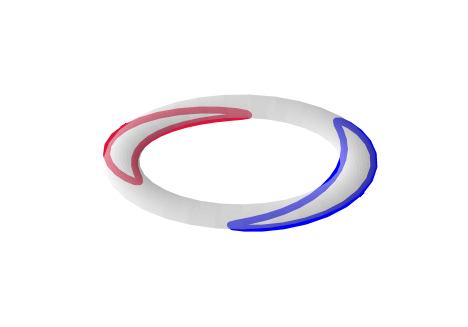
\includegraphics[width = 0.5\textwidth]{figures/solutions/ch9/torus.png}
    \caption{Slow manifold of the slowly forced pendulum. The torus shown is the $v=0$ section of phase space. The colored curves make up the slow manifold, the blue one is $\varphi_1(\psi)$ and the red one is $\varphi_2(\psi)$. }
    \label{fig:t}
\end{figure}
The slow manifold is shown in Fig. \ref{fig:t}. The red curve is the unstable part of $C_\varepsilon$ and the blue one is the stable part. 
They trace out closed curves, $\varphi_1$ oscillating between $-\text{arcsin}(F_0)$ and $\text{arcsin}(F_0)$ and $\varphi_2$ between $\pi + \text{arcsin}(F_0)$ and $\pi-\text{arcsin}(F_0)$. 
In the extended phase space, $S^1 \times S^1 \times \mathbb{R}$ (the torus shown is just a submanifold of this), 
the curve $\varphi_2$ has a local stable manifold and an unstable manifold. Trajectories in the stable manifold would converge to $\varphi_2$, while all other nearby trajectories would converge to $\varphi_1$. 
\end{solution}

\begin{solution}[9.7]
Stommel's model for the Thermohaline circulation is 
\begin{align}
   \label{eqstomm}
    \dot{x} &= -\frac{1}{\tau_x}(x-1) + \frac{1}{\tau_y}x[1+\eta^2(x-y)^2] \\
    \dot{y} & = \frac{\mu}{\tau_y} - \frac{1}{\tau_y}y[1+\eta^2(x-y)^2].
\end{align}
The variables are $x,y$, where $x(t)$ is the temperature-gradient and $y(t)$ is the salinity gradient. The parameter $\mu$ is the freshwater flux, $\eta$ is the nonlinear coupling constant. The relaxation times for the two processes are $\tau_x$ and $\tau_y$, which satisfy $\tau_x/\tau_y = \varepsilon \ll 1$.

(a) Show that Stommel's model has a globally attracting slow manifold that governs the asymptotic behavior of THC. Find a leading order approximation to this manifold. 

\emph{Solution}

Introducing the new timescale $s=t\tau_y$, $d/dt = 1/\tau_y d/ds$:
\begin{align*}
    \frac{1}{\tau_y}\frac{dx}{ds} &= -\frac{1}{\tau_x}(x-1) + \frac{1}{\tau_y}x[1+\eta^2(x-y)^2] \\
    \frac{1}{\tau_y}\frac{dy}{ds} & = \frac{\mu}{\tau_y} - \frac{1}{\tau_y}y[1+\eta^2(x-y)^2].
\end{align*}
Using the definition of $\varepsilon$, we have the singular perturbation problem, with $x$ the fast variable and $y$ the slow variable. 
\begin{align}
\label{eqfast1}
    \varepsilon\frac{dx}{ds} &= -(x-1) + \varepsilon x[1+\eta^2(x-y)^2]:=f(x,y,\varepsilon) \\
    \label{eqfast2}
    \frac{dy}{ds} & = \mu - y[1+\eta^2(x-y)^2] :=g(x,y).
\end{align}
Switching timescales again, by $s=\varepsilon \tau$ and denoting the differentiation with respect to $\tau$, by $(\cdot)'$ 
\begin{align*}
    x' &= -(x-1) + \varepsilon x[1+\eta^2(x-y)^2] \\
    y' & = \varepsilon\left(\mu - y[1+\eta^2(x-y)^2]\right).
\end{align*}
Setting $\varepsilon = 0$, we get the fast subsystem:
$$
x' = -(x-1) 
$$
and $y' = 0$.

We look for the fixed point of this subsystem, which is $x=1$, for any $y$, which means we can write the critical manifold as
\begin{equation}
    C_0 = \{ (x,y): x = 1\}. 
\end{equation}
The stability of the critical manifold depends on the stability of the fixed point $x=1$ in the fast subsystem. Since 

$$
\frac{d}{dx}f(x,y,0) = -1
$$
this fixed point is hyperbolic and also attracting with a rate $e^{-\tau}$. Because of this, the critical manifold $C_0$ is a normally attracting invariant manifold for the system, for $\varepsilon = 0$. 

As a result of Fenichel's theorem, we conclude that for small enough $\varepsilon$, there is a normally attracting invariant manifold $C_\varepsilon$ for the system (\ref{eqstomm}), which is $O(\varepsilon)$ close to $C_0$. This is the slow manifold, which we can represent as a graph

$$
C_\varepsilon = \{ (x,y): x = \varphi(y,\varepsilon)\}.
$$
Because of the smoothness properties, we can expand it in terms of $\varepsilon$: $x = \varphi(y,\varepsilon) = \varphi_0(y) + \varepsilon \varphi_1(y) + O(\varepsilon^2) = 1+\varphi_1(y)+O(y^2)$.


On one hand, on the manifold we have $x = \varphi(y,\varepsilon)$, which we can differentiate with respect to $\tau$.
\begin{equation}
    \label{eq11}
    x' = \frac{d \varphi}{d y} y' = \varepsilon^2 \frac{d\varphi_1(y)}{dy}\left( \mu- y -y\eta^2(1+\varepsilon\varphi_1(y) -y)^2\right) = O(\varepsilon^2).
\end{equation}

On the other hand, we can use the $x'$ equation restricted to the manifold. 
\begin{align*}
        \label{eq22}
    x' &= f(\varphi(y,\varepsilon),y,\varepsilon) = -\varepsilon \varphi_1(y) + \varepsilon x[1+\eta^2(x-y)^2]= \\
    &= -(x-1) + \varepsilon x[1+\eta^2(x^2-2xy + y^2)] = \\
    &= -\varepsilon\varphi_1(y) + \varepsilon + \varepsilon \eta^2(1-2y +y^2) +O(\varepsilon^2).
\end{align*}
For the manifold to be invariant, these two expressions must match in all orders of $\varepsilon$. Since in (\ref{eq11}), there were no order $\varepsilon$ terms, we must get 0 for the coefficient of the $O(\varepsilon)$ term in the latter expression. This means

$$
\varphi_1(y)= 1 + \eta^2(1-y)^2.
$$

To leading-order, the slow manifold is described by the graph $x = 1 + \varepsilon(1+\eta^2(1-y)^2)$.

(b) Compute the leading-order reduced flow on the slow manifold. Determine qualitatively the possible dynamical behaviors on the slow manifold as the parameters $\mu$ and $\eta$ are varied.

\emph{Solution}

To derive the reduced order flow, we Taylor-expand the equation governing the slow variable (on the original timescale, $s$):

\begin{equation*}
    g(x,y) = g(\varphi_0(y), y) + \varepsilon\left(\frac{d g}{dx}|_{(\varphi_0(y),y)}\right)\varphi_1(y) + O(\varepsilon^2)
\end{equation*}
From (\ref{eqfast2}), $g(x,y)= \mu - y[1+\eta^2(x-y)^2]$
$$
g(x,y) = \mu - y[1+\eta^2(1-y)^2] -2 \varepsilon\varphi_1(y)\eta^2y(1-y) + O(\varepsilon^2)
$$
Plugging in the expression for $\varphi_1$, we have

$$
g(x,y) = \mu - y[1+\eta^2(1-y)^2] -2 \varepsilon(1 + \eta^4y(1-y)^3) + O(\varepsilon^2)
$$
Keeping only the leading order term, we get the reduced dynamics on the slow manifold
$$
\frac{dy}{ds} = \mu - y[1+\eta^2(1-y)^2].
$$

On the slow manifold, the long time behavior of solutions is dictated by the fixed points. They are the roots of the right hand side:

$$
\mu = y[1+\eta^2(1-y)^2]
$$

The graph of these functions are shown in Fig. \ref{fig:c}. The fixed points of the system are given by the intersection points. 
\begin{figure}[h!]
    \centering
    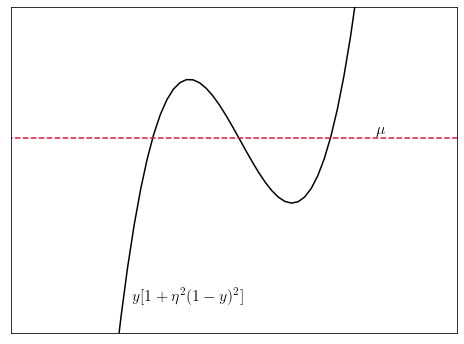
\includegraphics[width = 0.4\textwidth]{figures/solutions/ch9/cubic.png}
    \caption{Graphs of the functions $f(y) = \mu$ and $f(y)= y[1+\eta^2(1-y)^2]$.}
    \label{fig:c}
\end{figure}
To see the effect of the parameters, note that the shape of the cubic function is only governed by $\eta$. It can have at most two critical points, one minimum and one maximum. These are:
$$
\frac{d}{dy}y[1+\eta^2(1-y)^2] =0
$$

$$
1 + \eta^2(1-y)^2 - 2y \eta^2 (1-y) = 0
$$

$$
3\eta^2 y^2 - 4y\eta^2 +1 + \eta^2 = 0.
$$
This equation has two roots (the minimum and maximum of the cubic function) if 
$$
16\eta^4 - 12\eta^2(1+\eta^2) > 0,
$$
or $\eta^2 > 3$. In this case, the intersection of this graph with $y=\mu$ can give 1, 2 or 3 values. If $y$ is smaller or larger than any of the critical values of the graph, there is only one solution. In these cases the right hand side of the system $\mu - y[1+\eta^2(1-y)^2]$ changes sign at the fixed points, and they are stable. 

When $\mu$ reaches (one of) the critical values, a new fixed point appears in a bifurcation.

When $\mu$ is between the critical values, we have 3 fixed points, two stable and one unstable. 

When the above discriminant is 0, at $\eta^2 = 3$,  the cubic graph has only one critical point, and for all values of $\mu$ we only have one fixed point. This fixed point is stable. 
\end{solution}

\begin{solution}[9.8]
Assume $\lambda_s > 0$, then $Df(0)$ is diagonalizable with the matrix $T$, formed from the eigenvectors of $Df(0)$, $T= [e_{ss}, e_{s}]$

\begin{align}
T^{-1}Df(0)T = \begin{bmatrix}
-\lambda_{ss} & 0 \\
0 & -\lambda_{s}
 \end{bmatrix}.
\end{align}
Introducing a new variable $y$, defined by $x = Ty$, the differential equation reads,
\begin{align}
\dot{y} = T^{-1}\dot{x} = \begin{bmatrix} 
\dot{y}_{ss} \\ 
\dot{y}_{s}\end{bmatrix} = \begin{bmatrix}
-\lambda_{ss} y_{ss} + g_{ss}(y) \\
-\lambda_{s} y_{s} + g_{s}(y)
\end{bmatrix} \label{sol98one}   
\end{align}
where $g_s$ and $g_{ss}$ are of order $O(|y|^2)$:
\begin{align}
    \limsup_{|y|\to 0} \frac{|g_{s,ss}(y)|}{|y|^2}\leq K,
\end{align}
for some $K$. 
To characterize the strong stable manifold $W$, consider a modified form of \eqref{sol98one}. Outside a small neighborhood $B_\delta:=[-\delta, \delta] \times [-\delta, \delta]\subset \mathbb{R}^2$, the vector field is smoothly changed to a linear one. 

This construction is done by using $C^\infty$ bump-functions $\psi_\delta : \mathbb{R} \to \mathbb{R}$, with the properties 
\begin{align}
	\psi_\delta(r) &= 1 \text{ for } |r|\leq \delta \\
\psi_\delta(r) &\leq 1 \text{ for } \delta \leq |r|\leq 2\delta \\
\psi_\delta(r) &= 0 \text{ for } 2\delta \leq |r| \\
|\psi_\delta(r)'| &\leq \frac{K_0}{\delta}.
\end{align}

Then, define the new functions, the components of the modified nonlinear part of the vector field \eqref{sol98one} as 
\begin{align}
G_{s, ss}: \mathbb{R}^2 \to \mathbb{R}
\end{align}
\begin{align}
G_{s, ss}(y) := \psi_\delta(y_s)\psi_\delta(y_{ss})g_{s,ss}(y).
\end{align}

The gradient of this function is (with the notation $\psi = \psi_\delta(y_{ss})\psi_\delta(y_s)$)
\begin{align}
\nabla G_{s, ss}(y) = g_{s,ss}(y)\begin{bmatrix}\psi_\delta(y_s)'\psi_\delta(y_{ss}) \\ \psi_\delta(y_{ss})'\psi_\delta(y_s) \end{bmatrix} + \psi(y) \nabla g_{s,ss}(y).
\end{align}
The norm can be bounded by
\begin{align}
|\nabla G_{s, ss}(y) | \leq \sqrt{2}|g_{s,ss}|\frac{K_0}{\delta} + |\nabla g_{s,ss}(y)| \leq K_0 C \delta + C_1 \delta = K_2 \delta,
\end{align}
because of the properties of the bump functions and we use the fact that $|g_{s,ss}|$ can be bounded by a quadratic function on the region $B_\delta$. 

The modified vector takes the form  
\begin{align}
    \begin{bmatrix}
    \dot{y}_{ss} \\
    \dot{y}_{s} 
    \end{bmatrix} = \begin{bmatrix} -\lambda_{ss} y_{ss} + G_{ss}(y)\\ -\lambda_{s} y_{s} + G_{s}(y)\end{bmatrix}.
    \label{sol98two}
\end{align}
The strong stable manifold of system \eqref{sol98two} is $\overline{W}$, which coincides with the strong stable manfifold of the original system on $B_\delta$. It is distinguished by the property, that trajectories on the manifold decay at least as fast as $e^{-\gamma t}$ for positive times:
\begin{align}
W =\overline{W}\cap B_\delta = \left\{ y_0\in B_\delta : \sup_{t\geq 0} e^{\gamma t}|F^t(y_0)| < \infty \right \}.
\end{align}

To prove the existence of the strong stable manifold, we put system \eqref{sol98two} in a weak form, to make use of Banach's fixed point theorem. 

As seen in the lecture notes, the solutions of a system of the form
\begin{align}
\dot{x} = Ax + f(x,t)
\end{align}

are the solutions to the integral equation
\begin{align}
x(t) = e^{A(t-t_0)}x_0 + \int_{t_0}^t e^{A(t-\tau)}f(x(\tau),\tau)d\tau.
\end{align}

Applying this general form to system \eqref{sol98two}, we have
\begin{align}
y_{ss}(t) &= e^{-\lambda_{ss}(t-t_{ss})}y_{ss}(t_{ss}) + \int_{t_0}^t e^{-\lambda_{ss}(t-\tau)}G_{ss}(y(\tau))d\tau \\
\label{sol98five}
y_s(t) &= e^{-\lambda_s(t-t_s)}y_s(t_s) + \int_{t_0}^t e^{-\lambda_s(t-\tau)}G_s(y(\tau))d\tau. 
\end{align}

Assuming $W$ is nonempty, pick an initial point $(y_{ss}(t_{ss}), y_s(t_s))\in W$. It has the property 
\begin{align}
e^{\gamma \tau}|y_s(\tau)| \leq e^{\gamma \tau}|y(\tau)| < \infty, \text{ for } \tau \geq 0.
\end{align}
Moreover, the norm of the first term in \eqref{sol98five} can be written as
\begin{align}
e^{-\lambda_s(t-t_s)}|y_s(t_s)| = |y_s(t_s)|e^{\gamma t_s} e^{-\lambda_s t}e^{-\lambda_s t_s}e^{-\gamma t_s} = |y_s(t_s)|e^{\gamma t_s} e^{-\lambda_s t} e^{(\lambda_s - \gamma)t_s}.
\end{align}
Because $|y_s(t_s)|e^{\gamma t_s} e^{-\lambda_s t}$ stays bounded for given $t$, (using the previous line, with $\tau = t_s$) and $\lambda_s<\gamma$, we have 
\begin{align}
e^{-\lambda_s(t-t_s)}|y_s(t_s)| \to 0 \text{ as } t_s \to \infty.
\end{align}

Then, we can choose the initial times to be $t_s = \infty$ and $t_{ss}=0$. Also, $y_{ss}(0)$ is the first coordinate of the initial point of the trajectory, when it enters $B_\delta$, that is, we can write $y_{ss}(0)=\delta$ to obtain the integral equations

\begin{align}
\label{sol98six}
y_{ss}(t) &= e^{-\lambda_{ss}t}\delta + \int_{0}^t e^{-\lambda_{ss}(t-\tau)}G_{ss}(y(\tau))d\tau \\
\label{sol98seven}
y_s(t) &= - \int_{t}^\infty e^{-\lambda_s(t-\tau)}G_s(y(\tau))d\tau. 
\end{align}

Claim: The set 
\begin{align}
B : = \left \{ y(t): y\in C^0 ([0, \infty), B_\delta ), \quad  \sup_{t\geq 0} e^{\gamma t}|y(t)|\leq K <\infty \right \},
\end{align}

equipped with the metric 
\begin{align}
d(y_1, y_2) := \sup_{t\geq 0} |y_1 - y_2|e^{\gamma t}. 
\end{align}

becomes a complete metric space, on which the map
\begin{align}
\mathcal{F}_\delta  : B \to B,
\end{align}
defined by the integral equations \eqref{sol98six}, \eqref{sol98seven}
\begin{align}
\mathcal{F}_\delta (y) = \begin{bmatrix} e^{-\lambda_{ss}t}\delta + \int_{0}^t e^{-\lambda_{ss}(t-\tau)}G_{ss}(y(\tau))d\tau \\
- \int_{t}^\infty e^{-\lambda_s(t-\tau)}G_s(y(\tau))d\tau
\end{bmatrix}
\end{align}
is a contraction mapping, that is, for $q<1$, 
\begin{align}
d(\mathcal{F}_\delta(y_1), \mathcal{F}_\delta(y_2))\leq q d(y_1, y_2). 
\end{align}

First, we show that the map $d(y_1, y_2)$ is a metric, by showing that it satisfies the defining properties of a metric
\begin{align}
    d(y_1, y_2) &= 0 \text{ if and only if } |y_1-y_2|=0 \Longleftrightarrow y_1=y_2 \\
    d(y_1, y_2) &= \sup_{t\geq 0} |y_1 - y_2|e^{\gamma t} = \sup_{t\geq 0} |y_2 - y_1|e^{\gamma t} = d(y_2, y_1) \\
    d(y_1, y_3) &= \sup_{t\geq 0} |y_1 - y_3|e^{\gamma t} \leq  \sup_{t\geq 0} (|y_1 - y_2| + |y_2 - y_3|)e^{\gamma t} \\ &= \sup_{t\geq 0} |y_1 - y_2|e^{\gamma t} + \sup_{t\geq 0}  |y_2 - y_3|e^{\gamma t} = d(y_1,y_2) + d(y_2, y_3).
\end{align}

In the usual metric, a sequence of uniformly continuous functions does have a continuous limit. If, in addition, the sequence of functions is also bounded in this weighted sense, the limit will also have this property, which means that B is complete. 

Next, we show that the map $\mathcal{F}_\delta$ defined above maps to $B$. 
\begin{align}
|\mathcal{F}_\delta(y(t))| &\leq |y_s(t)| + |y_{ss}(t)| \\
			   &\leq \left|e^{-\lambda_{ss}t}\delta + \int_{0}^t e^{-\lambda_{ss}(t-\tau)}G_{ss}(y(\tau))d\tau \right| + \left|\int_{t}^\infty e^{-\lambda_s(t-\tau)}G_s(y(\tau))d\tau\right| \\    
&\leq e^{-\lambda_{ss}t}\delta + \int_{0}^t e^{-\lambda_{ss}(t-\tau)}|G_{ss}(y(\tau))|d\tau + \int_{t}^\infty e^{-\lambda_s(t-\tau)}|G_s(y(\tau))|d\tau.
\end{align}
Using the mean value theorem, and the bound developed above, 
\begin{align}
|\nabla G_{s,ss}| \leq g_{s,ss} \leq K_2\delta, \qquad |G_{s,ss}(y_{s,ss})| \leq  K_2\delta |y_{s,ss}|.
\end{align}
We can derive the following
\begin{align}
|\mathcal{F}_\delta(y(t))| &= e^{-\lambda_{ss}t}\delta + \int_{0}^t e^{-\lambda_{ss}(t-\tau)}|G_{ss}(y(\tau))|d\tau + \int_{t}^\infty e^{-\lambda_s(t-\tau)}|G_s(y(\tau))|d\tau \\
 &\leq e^{-\lambda_{ss}t}\delta + \int_{0}^t e^{-\lambda_{ss}(t-\tau)}K_2 \delta |y_{ss}(\tau)|d\tau + \int_{t}^\infty e^{-\lambda_s(t-\tau)}K_2 \delta |y_s(\tau )|d\tau. 
\end{align}
Multiply by $e^{\gamma t}$ and take the supremum
\begin{align}
\sup_{t\geq 0}|\mathcal{F}_\delta(y(t))|e^{\gamma t} &\leq \sup_{t\geq 0} \left \{ \delta e^{(\gamma -\lambda_{ss}) t}  + \int_{0}^t e^{-\lambda_{ss}(t-\tau)}K_2 \delta |y_{ss}(\tau)|e^{\gamma t}d\tau \right.\\
						     &\qquad \left.+ \int_{t}^\infty e^{-\lambda_s(t-\tau)}K_2 \delta |y_s(\tau )|e^{\gamma t}d\tau \right \}   \\
& \leq \sup_{t\geq 0} \left \{ \delta + \int_{0}^t e^{-\lambda_{ss}(t-\tau)}K_2 \delta |y_{ss}(\tau)|e^{\gamma \tau} e^{-\gamma \tau }e^{\gamma t}d\tau \right.\\
&\qquad \left.+ \int_{t}^\infty e^{-\lambda_s(t-\tau)}K_2 \delta |y_s(\tau )|e^{\gamma \tau} e^{-\gamma \tau }e^{\gamma t}d\tau\right \} \\
&\leq \sup_{t\geq 0} \left \{ \delta +  K_2 \delta K\int_{0}^t e^{(t-\tau)(\gamma - \lambda_{ss})} d\tau +  K_2 \delta K\int_{t}^\infty e^{(t-\tau)(\gamma - \lambda_s)} d\tau\right \}.
\end{align}
After carrying out the integrals, and using $\gamma -\lambda_{ss} < 0$ and $\gamma-\lambda_s> 0$
\begin{align}
\sup_{t\geq 0}|\mathcal{F}_\delta(y(t))|e^{\gamma t} &\leq 
\sup_{t\geq 0} \left \{ \delta +  K_2 \delta K \left [ \frac{1}{\lambda_{ss} - \gamma}e^{(t-\tau)(\gamma - \lambda_{ss})}\right]_0^t\right.\\
						     &\qquad \left.+ K_2 \delta K \left [ \frac{1}{\lambda_{s} - \gamma}e^{(t-\tau)(\gamma - \lambda_{s})}\right]_t^\infty \right \}   \\
&=  \sup_{t\geq 0} \left \{ \delta +  K_2 \delta K  \frac{1 - e^{t(\gamma - \lambda_{ss})}}{\lambda_{ss} - \gamma} + K_2 \delta K \frac{1}{\gamma - \lambda_{s} }\right \}  \\
& \leq \delta +  K_2 \delta K \left( \frac{1}{\lambda_{ss} - \gamma} + \frac{1}{\gamma - \lambda_{s} }\right)\\ 
&= K \left[\frac{\delta}{K}+K_2 \delta \left( \frac{1}{\lambda_{ss} - \gamma} + \frac{1}{\gamma - \lambda_{s} }\right) \right ].
\end{align}
Choosing $\delta$, such that
\begin{align}
\delta \leq \frac{1}{\frac{1}{K}+K_2 \left( \frac{1}{\lambda_{ss} - \gamma} + \frac{1}{\gamma - \lambda_{s} }\right) },
\end{align}
guarantees that 
\begin{align}
\sup_{t\geq 0}|\mathcal{F}_\delta(y(t))|e^{\gamma t} \leq K < \infty,
\end{align}
which shows that the image of a function $y\in B$ under the functional $\mathcal{F}$ is still in $B$. 

So far we have established that $B$ is a complete metric space and $\mathcal{F}$ is a map from $B$ to $B$. To show that $\mathcal{F}$ is a contraction mapping, consider the difference between two image-points in $B$
\begin{align}
    |\mathcal{F}(y_1) - \mathcal{F}(y_2)| &= \left \vert\int_{0}^t e^{-\lambda_{ss}(t-\tau)}[G_{ss}(y_1(\tau)) - G_{ss}(y_2(\tau))]d\tau \right \vert \\
					  &\quad+  \left \vert \int_{t}^\infty e^{-\lambda_s(t-\tau)}[G_{s}(y_1(\tau)) - G_{s}(y_2(\tau))]d\tau \right \vert \\
    & \leq \int_{0}^t e^{-\lambda_{ss}(t-\tau)}|[G_{ss}(y_1(\tau)) - G_{ss}(y_2(\tau))]|d\tau  \\
    &\quad +  \int_{t}^\infty e^{-\lambda_s(t-\tau)}|[G_{s}(y_1(\tau)) - G_{s}(y_2(\tau))] | d\tau  \\
    & \leq \int_{0}^t e^{-\lambda_{ss}(t-\tau)}K_2 \delta |y_1(\tau) - y_2(\tau)|d\tau \\ 
    &\quad +  \int_{t}^\infty e^{-\lambda_s(t-\tau)}K_2\delta |y_1(\tau) - y_2(\tau) | d\tau.
\end{align}

Multiplying by $e^{\gamma t}$
\begin{align}
    |\mathcal{F}(y_1) - \mathcal{F}(y_2)|e^{\gamma t} &\leq \int_{0}^t e^{-\lambda_{ss}(t-\tau)}K_2 \delta |y_1(\tau) - y_2(\tau)|e^{\gamma t}d\tau  \\
						      &\quad+  \int_{t}^\infty e^{-\lambda_s(t-\tau)}K_2\delta |y_1(\tau) - y_2(\tau) |e^{\gamma t} d\tau  \\
    & = \int_{0}^t e^{-\lambda_{ss}(t-\tau)}K_2 \delta |y_1(\tau) - y_2(\tau)|e^{\gamma \tau} e^{\gamma t} e^{-\gamma \tau}d\tau  \\
    &\quad+ \int_{t}^\infty e^{-\lambda_s(t-\tau)}K_2\delta |y_1(\tau) - y_2(\tau) |e^{\gamma \tau} e^{\gamma t} e^{-\gamma \tau} d\tau \\
    &\leq \int_{0}^t e^{(\gamma-\lambda_{ss})(t-\tau)}K_2 \delta d\tau \sup_{t\geq 0} |y_1(t) - y_2(t) |e^{\gamma t}  \\
    &\quad+ \int_{t}^\infty e^{(\gamma-\lambda_s)(t-\tau)}K_2\delta d\tau \sup_{t\geq 0} |y_1(t) - y_2(t) |e^{\gamma t} \\
    & = K_2 \delta d(y_1, y_2) \left (\int_{0}^t e^{(\gamma-\lambda_{ss})(t-\tau)}d\tau + \int_{t}^\infty e^{(\gamma-\lambda_s)(t-\tau)} d\tau \right) \\
    \end{align}
    Thus we can surmise
\begin{align}
    \sup_{t\geq0}|\mathcal{F}(y_1) - \mathcal{F}(y_2)|e^{\gamma t}&\leq \delta K_2 d(y_1, y_2) \left( \frac{1}{\lambda_{ss} - \gamma} + \frac{1}{\gamma - \lambda_{s} }\right).
\end{align}

If we choose $\delta$ such that 
\begin{align}
\delta < \frac{1}{K_2 \left( \frac{1}{\lambda_{ss} - \gamma} + \frac{1}{\gamma - \lambda_{s} }\right)}
\end{align}
then we obtain the contraction-mapping criterion for $q<1$. Also note that if $\delta$ satisfies the earlier inequality, it automatically satisfies the contraction mapping criterion too. 

Then, we can use Banach's fixed point theorem, and conclude that $\mathcal{F}$ has a unique fixed point in $B$, which, by construction must coincide with the strong stable manifold of the origin, within the small neighborhood $B_\delta$, which was to be proved. 


	
\end{solution}

